\chapter{Results}
\label{ch:res}
In this chapter, we use the forward model to generate data given an underlying ground truth and then guide the reader towards obtaining the posterior distributions.
Once we simulated some data, we established a Bayesian framework in Sec. \ref{sec:BayModel}, where we discuss the choice of prior distributions and formulate the posterior distributions for ozone and pressure over temperature, respectively.
Since our forward model is weakly non-linear we like to approximates the non-linear forward model $\bm{A}_{NL} \approx \bm{M} \bm{A}_{NL}$ with an affine map $\bm{M}$, see Sec. \ref{sec:affineMap}.
In doing so, we sample from the marginal posterior for ozone and compare that to the tensor-train (TT) approximation.
Then we calculate the mean and the covariance matrix of the full conditional posterior and use the obtained posterior ozone samples to create two affine subspaces, to which we map in between.
Finally, we calculate the posterior distribution for ozone and pressure over temperature with the updated forward map $\bm{A} = \bm{M} \bm{A}_{NL}$ and compare to a ground truth.
Lastly, we evaluate some errors occurring during the process.
All programming and analysis are done in Python on a MacBook Pro from 2019 with a 2.4 GHz quad-core Intel Core i5 processor.

\section{Simulate Data based on a ground truth}
We take a ground truth ozone profile generated from some data \cite{MLSdata} of the microwave limb sounder on the aura satellite in the Antarctic region with a peak in high altitude (to show that the data is uninformative in those regions), see Fig. \ref{fig:O3Samp}.
The ozone profile from \cite{MLSdata} provides ozone volume mixing ratios versus pressure, so we recursively calculate the geometric height with the hydrostatic equilibrium equation
\begin{align}
	\frac{\text{d}p}{p} = \frac{- g M}{R^* T} \text{d} h \, ,
\end{align}
with the acceleration due to gravity
\begin{align}
	g = g_0 \Bigg( \frac{r_0}{r_0 + h} \Bigg) \, ,
\end{align}
where the polar radius pf the earth is $r_0 \approx 6356 \, \text{km}$, the gravitation at sea level is $g_0 \approx 9.81 \text{m}/\text{s}^2$, $R^* = 8.31432 \times 10^{-3} \text{Nm} / \text{kmol} / \text{K}$ and the mean molecular weight of the air is $M = 28.97 \text{kg/kmol}$ \cite{atmosphere1976us}.
This holds up to a geometric height of $86$km, where ignore a $0.04\%$ change in $M$ from $80$km to $86$km in geometric altitude.

Following \cite{atmosphere1976us} we form a temperature function
\begin{align}
	T(h) = \begin{cases*}
			T_0 &, \, \text{$h  = 0$}\\
			T_0 + a_0 h   &, \, \text{$0 \leq h < h_{1}$}\\
			T_0 + a_0 h_{1} &, \, \text{$h_{1} \leq  h < h_{2}$}\\
			T_0 + a_0 h_{1} + a_1 (h_2   - h_1)  + a_2 (h   - h_2)  &,  \, \text{$h_{2} \leq h < h_{3}$}\\
			T_0 + a_0 h_{1} + a_1 (h_2   - h_1)  + a_2 (h_3   - h_2) + a_3 (h   - h_3) &, \, \text{$h_{3} \leq h < h_{4}$}\\
			T_0 + a_0 h_{1} + a_1 (h_2   - h_1)  + a_2 (h_3   - h_2) + a_3 (h_4   - h_3)&\nonumber \\
			\hphantom{{} T_0 } + a_4 (h   - h_4) &,  \, \text{$h_{4} \leq h < h_{5}$}\\
			T_0 + a_0 h_{1} + a_1 (h_2   - h_1)  + a_2 (h_3   - h_2) &\nonumber \\
			\hphantom{{} T_0 } + a_3 (h_4   - h_3) + a_4 (h_5   - h_4)+ a_5 (h   - h_5) &,  \, \text{$h_{5} \leq h < h_{6}$}\\
			T_0 + a_0 h_{1} + a_1 (h_2   - h_1) + a_2 (h_3   - h_2)  &\nonumber\\
			\hphantom{{} T_0} + a_3 (h_4   - h_3) + a_4 (h_5   - h_4)+ a_5 (h_6   - h_5)  &,  \, \text{$h_{6} \leq h \lesssim 86$}
	\end{cases*} 
\label{eq:tempFunc}
\end{align}
with gradient and height values provided by \cite{atmosphere1976us}, see Tab. \ref{tab:tempGrad}, which act as the ground truth temperature, see Fig. \ref{fig:PriorTemp}.
\begin{table}
	\centering
	\begin{tabular}{ |c||c|c|  }
		\hline
		subscript $i$ & geometric height $h_i$ in km&gradient $a_i$\\
		\hhline{|=||=|=|}
		0& 0 & -6.5\\
		1& 11 & 0\\
		2& 20.1& 1\\
		3& 32.2& 2.8\\
		4& 47.4& 0\\
		5& 51.4& -2.8\\
		6& 71.8& -2\\
		\hline
	\end{tabular}
\caption[Temperature gradients]{Definition of height depending temperature gradients.}
\label{tab:tempGrad}
\end{table}

Then we can compute a data vector $\bm{y}$, with $m = 42$ measurements according to the radiative transfer equation (RTE), see Eq. \ref{eq:RTE}, determined by the satellite pointing accuracy of $150$arcsec as requested by the internal report of the proposed cube-satellite \cite{CubeSatInternal}, within an atmosphere $h_{L,0}=7$km and $h_{L,n} = 83.3$km with $n = 45$ layers.
The height values $h_{L,i}$ for each layer $i = 0,\dots, n$ are defined by the ozone profile from \cite{MLSdata} and its pressure values.
We target thermal radiation at a wave number $\nu = 7.86\text{cm}^{-1}$, equal to a frequency of roughly $235$GHz, where we assume that ozone is the only emitter at that frequency, see \cite{}, and calculate the absorption constant $k(\nu,T)$ as in Eq. \ref{eq:absRTE}, following the \textit{HITRAN} database \cite{gordon2022hitran2020}, which provides the line intensity $L(\nu,T_{\text{ref}})$ for the isotopologue $\prescript{16}{}{\text{O}}_3$ with the AFGL Code 666.
Lastly we add normally distributed $\bm{\nu} \sim \mathcal{N}(0,\gamma^{-1} \bm{I})$ noise so that we have a voltage Signal-to-Noise (SNR) of $60$, similar to THz module on the MLS aura satellite \cite{pickett2006snr}.
\begin{align}
	\text{SNR} = \frac{max(y)}{std noise} = \frac{max(y)}{std noise}
\end{align}
Note that we multiply the data with $10^{11}$ to avoid numerical issues within the inversion process.
Can also see that when we plot the data
\begin{figure}[ht!]
	\centering
	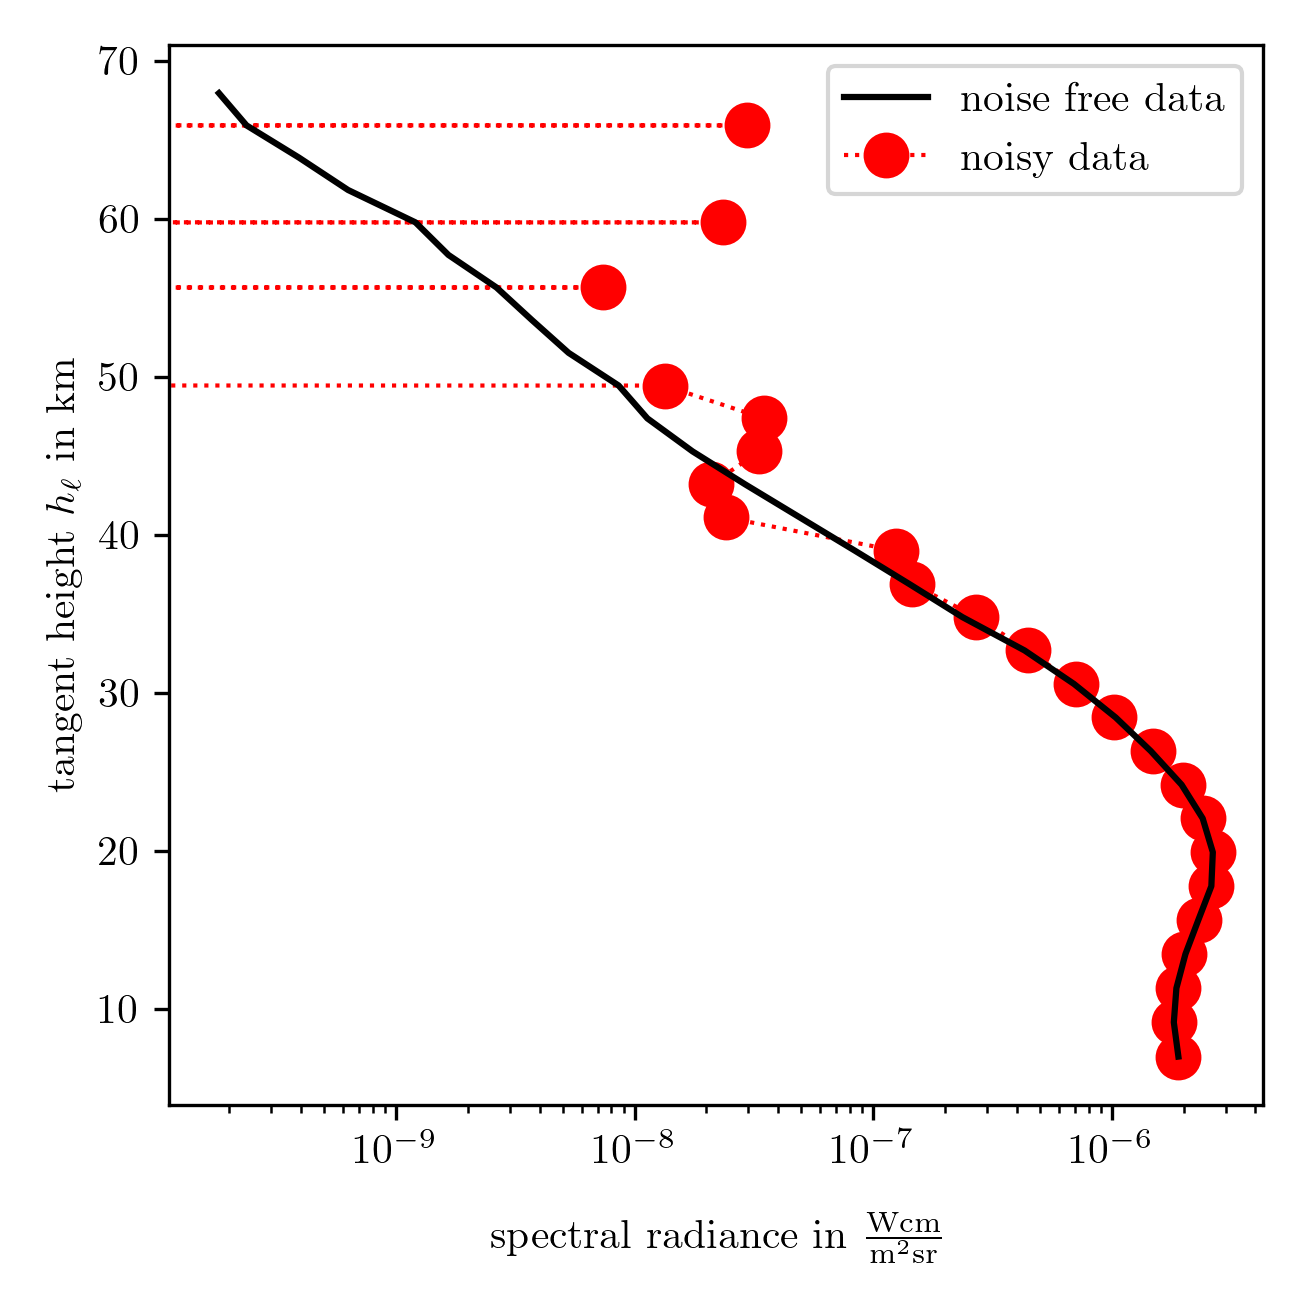
\includegraphics{DataPlot.png}
	\caption[Logarithmic plot of data points at different tangent height.]{Logarithmic plot of data points at different tangent height. Note that negative values are not appearing and we see that at a caertein heitgh noise is dominating.}
	\label{fig:}
\end{figure}.
Now, given the data, we want to invert the process and determine a posterior distribution over the ozone $\bm{x}$, pressure $\bm{p}$ and temperature $\bm{T}$.

\section{Set up a hierarchical Bayesian framework}
\label{sec:BayModel}
Since the forward model described in Ch. \ref{ch:formodel} is weakly non-linear we will set up a linear Bayesian hierarchical framework first based on the linear forward model $\bm{A}_L$ and then later the approximated version $\bm{A}_{NL}\bm{M} \bm{A}_L$.
Furthermore, the noise is normally distributed, so we establish a linear-Gaussian Bayesian hierarchical framework, aiming to recover an ozone profile and a pressure over temperature profile.
In doing so, we first draw a directed acyclic graph (DAG) to visualise the measurement and modelling process and determine hyper-parameters and correlations between parameters.
Then we define prior distributions over all parameters as well as a likelihood function so that we can formulate the posterior distribution.


\begin{figure}[thb!]
	\centering
	\begin{tikzpicture}
		\node[roundnode2] at (-4.5,6.5) (Q)     {$\bm{Q}$};
		\node[roundnode2] at (-3,5) (x)     {$\bm{x}$};
		\node[align=center] at (-1,4) (A)    {$\bm{A}_{NL} \approx  \bm{M}\bm{A}_L$};
		\node[roundnode2] at (-1,2.5) (u)    {$\bm{\Omega}$};
		\node[rectnode] at (-1,1) (y)    {$\bm{y}$};
		\node[roundnode2] at (-2.5,2.5) (e)    {$\bm{\eta}$};
		\node[roundnode2] at (-6.25,6.5) (S)    {$\bm{\Sigma}$};
		\node[roundnode2] at (-7.75,8) (s)    {$\gamma$};
		\node[roundnode2] at (-6,8) (d)    {$\delta$};
		\node[roundnode2] at (3,6.5) (t)     {$\bm{T}$};
		\node[roundnode2] at (-1,6.5) (p)     {$\bm{p}$};
		\node[roundnode2] at (1,5) (pt)     {$\bm{p}/\bm{T}$};
		\node[roundnode2] at (0,8) (b1)    {$b$};
		%\node[roundnode2] at (1,8) (b2)    {$b_2$};
		%\node[roundnode2] at (-2,8) (h1)    {$h_{0}$};
		\node[roundnode2] at (-1.5,8) (p0)    {$p_0$};
		\node[roundnode2] at (2.25,8) (ht)    {$\bm{h_T}$};
		\node[roundnode2] at (3.25,8) (ct)    {$T_0$};
		\node[roundnode2] at (4.25,8) (at)    {$\bm{a}$};
		
		\node[roundnode2] at (0,10) (b1hyp)    {$\bm{\theta}_{b}$};
		%\node[roundnode2] at (-2.5,10) (h1hyp)    {$\bm{\theta}_{h_{0}}$};
		\node[roundnode2] at (-1.5,10) (p0hyp)    {$\bm{\theta}_{p_{0}}$};
		\node[roundnode2] at (2,10) (hthyp)    {$\bm{\theta}_{\bm{h}}$};
		\node[roundnode2] at (3.25,10) (cthyp)    {$\bm{\theta}_{T_{0}}$};
		\node[roundnode2] at (4.5,10) (athyp)    {$\bm{\theta}_{\bm{a}}$};
		
		\node[roundnode2] at (-7.75,10) (shyp)    {$\bm{\theta}_{\gamma}$};
		\node[roundnode2] at (-6,10) (dhyp)    {$\bm{\theta}_{\delta}$};
		
		%Lines
		
		
		\draw[->, very thick] (S) -- (e);
		\draw[->, mydotted, very thick] (s) -- (S);
		\draw[->, very thick] (u) -- (y);
		\draw[->, mydotted, very thick] (A) -- (u);
		\draw[->, mydotted,  very thick] (x) -- (A.north west);
		\draw[->, mydotted, very thick] (p) -- (pt);
		\draw[->, mydotted, very thick] (t) -- (pt);
		\draw[->, mydotted, very thick] (pt) -- (A.north east);
		%\draw[->, mydotted, very thick] (h1) -- (p);
		\draw[->, mydotted, very thick] (p0) -- (p);
		\draw[->, mydotted, very thick] (b1) -- (p); 
		%\draw[->, very thick] (b2.south) -- (p.east); 
		\draw[->, mydotted, very thick] (d) -- (Q); 
		\draw[->, mydotted, very thick] (e) -- (y); 
		
		\draw[->, very thick] (Q.south east) -- (x.north west); 
		\draw[->, mydotted, very thick] (ht.south) -- (t.north west);
		\draw[->, mydotted, very thick] (ct.south) -- (t.north);
		\draw[->, mydotted, very thick] (at.south) -- (t.north east);
		
		
		\draw[->, very thick] (b1hyp) -- (b1);
		%\draw[->, very thick] (h1hyp) -- (h1);
		\draw[->, very thick] (p0hyp) -- (p0);
		\draw[->, very thick] (hthyp) -- (ht);
		\draw[->, very thick] (cthyp) -- (ct);
		\draw[->, very thick] (athyp) -- (at);
		\draw[->, very thick] (shyp) -- (s);
		\draw[->, very thick] (dhyp) -- (d);
		
		
	\end{tikzpicture} 
	\caption[Complete directed acyclic graph of the forward model.]{Complete directed acyclic graph of the forward model. The hyper-parameters at the top deterministically (dotted line) describe the parameters ($\bm{p}/\bm{T}$) or the noise covariance $\bm{\Sigma} = \gamma^{-1} \bm{I}$ of the random (solid line) noise $\bm{\eta} \sim \mathcal{N}(0,\gamma^{-1} \bm{I} ) $ and precision matrix $\bm{Q} = \delta \bm{L}$ of the distribution of $\bm{x}\sim \mathcal{N}(0,\delta \bm{L}) $, where $\bm{L}$ is a graph Laplacian as in Eq. \ref{eq:GLapl}. We can group the noise precision $\gamma$  and the smoothness parameter $\delta$ to define the marginal posterior over those hyper-parameters and then condition on them for the conditional posterior distribution,for further details see Fig. \ref{fig:DAGO3}. In this whole process where we condition on the pressure $\bm{p}$ and temperature $\bm{T}$, which we retrieve separately, see Fig. \ref{fig:DAGPT}. The hyper-parameters $h_0,p_0,b$ deterministically describe the pressure function in Eq. \ref{eq:pressFunc}, note that we only need three parameters here since $h_0< h_{L,0}$ and $\bm{h}= \{ h_1, h_2,h_3,h_4,h_5,h_6\}$, $\bm{a} = \{ a_0, a_1, a_2,a_3,a_4\}$ and $T_0$ determine the temperature function.
		The parameters $\bm{x}$ and $\bm{p}/ \bm{T}$ determine the space of all measurable noise free data $\bm{\Omega}$ through the forward model $\bm{A}(\bm{x},\bm{p},\bm{T})$ from which we randomly observe data set plus some random noise.}
	\label{fig:DAGComplete}
\end{figure}


We draw a DAG for the measurement and modelling process, where the hyper-hyper-parameters $\theta_{\gamma}, \theta_{\delta},\theta_{p_0},\theta_{b},\theta_{\bm{h}},\theta_{T_0},\theta_{\bm{a}}$ in the top row of Fig. \ref{fig:DAGComplete} determine the hyper-prior distributions $\pi(\gamma, \delta, p_0, b, \bm{h}_T, \bm{T}_0, \bm{a})$ statistically (solid line).
Then the hyper-parameters determine the parameters $\bm{p}/\bm{T}$ deterministically.
The temperature function $\bm{T} = (T_0,\bm{a}, \bm{h}_T)$, Eq. \ref{eq:tempFunc}, is determined through $\bm{a}$ the temperature gradients at heights $\bm{h}$, see Tab. \ref{tab:tempGrad}, where $h_0$ is set to zero as we model temperature variability at the sea-level temperature trough the an additional input $T_0$.
Note that we define an exponential pressure function, Eq. \ref{eq:pressFunc}, later in Sec. \ref{subsec:presTempPrior} so that $\bm{p}(p_0,b)$ is defined through the hyper-parameters $p_0$ (pressure at sea-level) and $b$ (exponential gradient).
Since we do not parametrise the ozone profile, we assume a certain smoothness defined through the smoothness hyper-parameter $\delta$ and a precision matrix $\bm{Q}(\delta)$ which statistically defines a distribution over $\bm{x}$ (solid lines).
The parameters $\bm{x}, \bm{p},\bm{T}$ progress deterministically, see RTE in Eq. \ref{eq:RTE}, into the forward model $\bm{A}_{NL}$ and generate a space of all possible noise free data $\bm{\Omega}$.
From that space of all measurable $\bm{\Omega}$ we pick one data set to which we add some noise $\bm{\eta} \sim \mathcal{N}(0, \bm{\Sigma})$, which is modelled through the hyper-parameter $\gamma$ and the precision matrix $\bm{\Sigma} = \gamma^{-1} \bm{I}$ so that we obtain the noisy data vector $\bm{y}$.
Since the noise is normally distributed, so is the likelihood function $\pi(\bm{y} | \bm{x}, \bm{p}, \bm{T})$.
Then the joint posterior distribution
\begin{align}
	\pi(p_0,b,\bm{h_T},\bm{a},\delta, \gamma, \bm{x}| \bm{y}) \propto \pi(\bm{y} | \bm{x}, \bm{p}, \bm{T}) \pi(p_0,b,\bm{h_T},\bm{a},\delta, \gamma) 
\end{align}
over all 17 hyper-parameters and the parameter $\bm{x} \in \mathbb{R}^{45}$ is 62 dimensional.
Ideally, we characterise the joint posterior, but this is computationally not feasible.
Instead, we factorise the posterior into
\begin{align}
	\pi(p_0,b,\bm{h_T},\bm{a},\delta, \gamma, \bm{x}| \bm{y}) = \pi(\delta, \gamma, \bm{x}| p_0,b,\bm{h_T},\bm{a},\bm{y}) \pi(p_0,b,\bm{h_T},\bm{a}|\delta, \gamma, \bm{x}, \bm{y}) \, , 
\end{align}
where we either condition on ozone $\bm{x}$ and the smoothness hyper-parameter $\delta$ as well as the noise hyper-parameter $\gamma$ or on the fraction $\bm{p}/\bm{T}$, pressure over temperature, and its hyper-parameters.
Again as in Sec. \ref{ch:formodel} for brevity we write $\pi(p_0,b,\bm{h_T},\bm{a}| \gamma,\bm{y}) $ and $\pi(\delta, \gamma, \bm{x}|\bm{y})$, which implies that we conditioned on $\bm{x}$ or $\bm{p}$ and $\bm{T}$. 
Next, we need to specify the prior distribution, which we summarise in Tab. \ref{tab:priors}, to formulate the posterior distributions.
\begin{table}
	\centering
	\begin{tabular}{ |c||c|c|c|c|c|   }
		\hline
		& &\multicolumn{2}{|c|}{TT bounds}& &\\
		\hline
		model parameters& priors&\makecell{lower}& \makecell{upper\\
		}&$\tau_{\text{int}}$&Context\\
		\hhline{|=||=|=|=|=|=|}
		$\gamma$ & $\mathcal{T}(1,10^{-10})$ &$5 \, 10^{-8}$ &$4.5 \, 10^{-7}$&  $ 9\pm 0.1$ &$\bm{y}$\\ \hline
		$\delta$ &$\mathcal{T}(1,10^{-10})$ & -&-& $1.5 \pm 0.1$ & $\bm{x}$\\ \hline
		$\lambda$ &- & 500&$10^4$& $3.5 \pm 0.3$ &$\bm{x}$\\ \hline
		$\bm{x}$ &$\mathcal{N}(0,\delta \bm{L})$ & -&-&& $\bm{x}$\\ \hhline{|=||=|=|=|=|=|}
		%$\gamma$ & $\mathcal{N}(2.58e-9,2.58e-11)$ &2.45e-9&2.7e-9 &$\bm{x}$\\
		%$\delta_0$ &  $\mathcal{N}(0.8e-4,0.75e-5)$& 4e-5 & 1.1e-4&$\bm{x}$\\
		%$a_0$ &  $\mathcal{T}(3,1e6)$& 1e-15&1e-5&$\bm{x}$\\ \hline
		%$h_0$ &  $\mathcal{N}(31.35,1)$&27 &35&$\bm{x}$\\ \hline
		%$h_0$ &  $\mathcal{N}(5.5,0.5)$& 4.76&5.74&&$\bm{p/T}$\\ \hline
		%$b_2$ & $\mathcal{N}(0.13,0.067)$& 0&0.32&$\bm{p/T}$\\ \hline
		$h_{1}$ &  $\mathcal{N}(11,0.5)$&9.5 &12.5&$1820 \pm 49$ &$\bm{p/T}$\\ \hline
		$h_{2}$ &  $\mathcal{N}(20.1,1.6)$&17.7 &22.3&$454 \pm 7$&$\bm{p/T}$\\ \hline
		$h_{3}$ &  $\mathcal{N}(32.3,2.5)$&25.2&39.8&$394 \pm 5$&$\bm{p/T}$\\ \hline
		$h_{4}$ &  $\mathcal{N}(47.4,5)$&45.9 &48.9&$324 \pm 4$&$\bm{p/T}$\\ \hline
		$h_{5}$ &  $\mathcal{N}(51.4,5)$&49.9 &52.9&$319 \pm 4$&$\bm{p/T}$\\ \hline
		$h_{6}$ &  $\mathcal{N}(71.8,3)$&62.5 &80.8&$347 \pm 5$&$\bm{p/T}$\\ \hline
		$a_{0}$ &  $\mathcal{N}(-6.5,0.01)$&-6.53 &-6.47&$330 \pm 4$&$\bm{p/T}$\\ \hline
		$a_{1}$ &  $\mathcal{N}(0,0.1)$&-0.3 &0.3&$508 \pm 8$&$\bm{p/T}$\\ \hline
		$a_{2}$ &  $\mathcal{N}(1,0.01)$&0.97 &1.03&$341 \pm 5$&$\bm{p/T}$\\ \hline
		$a_{3}$ &  $\mathcal{N}(2.8,0.1)$&2.5 &3.1&$316 \pm 4$&$\bm{p/T}$\\ \hline
		$a_{4}$ &  $\mathcal{N}(0,0.1)$&-0.3 &0.3&$335 \pm 4$&$\bm{p/T}$\\ \hline
		$a_{5}$ &  $\mathcal{N}(-2.8,0.1)$&-3.1 &-2.5&$335 \pm 4$&$\bm{p/T}$\\ \hline
		$a_{6}$ & $\mathcal{N}(-2,0.01)$ &-2.03 &-1.97&$320 \pm 4$&$\bm{p/T}$\\ \hline
		$T_{0}$ &  $\mathcal{N}(288.15,4.5)$& 275 &302&$2446 \pm 76$&$\bm{p/T}$\\ \hline
		$b$ &  $\mathcal{N}(0.167,5\,10^{-4})$& 0.165& 0.171 &$2813 \pm 92$&$\bm{p/T}$\\ \hline
		$p_0$ &  $\mathcal{N}(1243,5)$&1229 &1259&$550 \pm 9$&$\bm{p/T}$\\ 
		\hline
	\end{tabular}
	\caption[Summary of relevant parameter characteristics, bounds and sampling statistics.]{Summary of relevant parameter characteristics, bounds and sampling statistics. We denote $\mathcal{N}(\mu,\sigma)$ as the Gaussian and $\mathcal{T}(\alpha = \text{scale}, \beta = \text{rate})$ as the gamma distribution. The IACT $\tau_{\text{int}}$ is estimated as in \cite{UwerrM} from posterior samples based on the approximated forward map.}
	\label{tab:priors}
\end{table}

\subsection{Ozone conditioned on pressure and temperature}
\label{subsec:OzoneSetup}
In this section, we choose prior distributions and describe the approach to evaluate the posterior distribution for ozone $\pi(\delta, \gamma, \bm{x}|\bm{y})$, including the noise hyper-parameter $\gamma$.
Assuming Gaussian noise $\bm{\eta} \sim \mathcal{N}(0, \gamma^{-1} \bm{I})$, we define a linear-Gaussian Bayesian hierarchical model~\cite{fox2016fast}
\begin{subequations}
	\begin{align}
		\bm{y} |  \bm{x}, \gamma &\sim \mathcal{N}(\bm{A} \bm{x}, \gamma^{-1} \bm{I}) \label{eq:likelihood} \\
		\bm{x} |  \delta &\sim \mathcal{N}(0, \delta \bm{L}) \label{eq:xPrior} \\
		\delta, \gamma &\sim \pi(\delta, \gamma) \label{eq:gammaPrior},
	\end{align}
	\label{eq:BayMode}
\end{subequations}
with a normally distributed likelihood $\pi(\bm{y} |  \bm{x}, \gamma)$ including the forward model matrix $\bm{A}$ and prior distributions $\pi(\bm{x} |  \delta)$ and $\pi(\delta, \gamma)$, the noise covariance matrix $\gamma^{-1} \bm{I}$, the prior precision matrix $\delta \bm{L}$ and the prior mean set to $\bm{0}$.
The chosen Bayesian model is very similar to a regularisation problem, since we like to show that regularisation is depreciated, and we are able to receive much more meaningful results compared to a regularisation approach.

\subsubsection{Prior Modelling}
To complete the Bayesian framework, we have to define prior distributions over the hyper-parameters and parameters.
Ideally, we define the prior distributions as uninformative as possible, and include functional dependencies and physical properties.

First, we set the precision matrix of the prior distribution $\bm{x}|\delta$ to
\begin{align}
	\delta \bm{L} =
	\delta
	\begin{bmatrix}
		2 & -1 & & &  \\
		-1 & 2 & -1 & &   \\
		& \ddots & \ddots & \ddots &\\ 
		& & -1 & 2 & -1  \\
		& & & -1 & 2 
	\end{bmatrix} 
	\label{eq:GLapl} 
\end{align}
which is the 1-dimensional Graph Laplacian as in \cite{wang2015graphs,fox2016fast} with Dirichlet boundary condition.
This matrix will also act as the regulariser later in the Regularisation section, see Sec. \ref{sec:regularise}.
For $\delta$ and $\gamma$ we pick  relatively uninformative gamma distributions so that $\gamma \sim \mathcal{T}(\bm{\theta_{\gamma}}) $ and $\delta \sim \mathcal{T}(\bm{\theta_{\delta}})$, where $\bm{\theta_{\gamma}} = \bm{\theta_{\delta}} = (1,10^{-10})$, see Fig. \ref{fig:MargPostHistTT}.
These gamma distributions have another advantage when sampling from the marginal posterior distribution $\pi(\gamma,\delta | \bm{y})$, where $\pi(\gamma | \lambda, \bm{y}) \sim \mathcal{T}(\cdot)$ with the regularisation parameter $\lambda = \delta / \gamma $.
We plot the corresponding prior ozone profiles according to $\bm{x}\sim \mathcal{N}(0, \delta \bm{L})$ in Fig. \ref{fig:O3Prior} and like to note that we should not include negative ozone values but are currently not able to include e.g. a truncated multivariate normal prior distribution for $\bm{x}$. 



\subsubsection{posterior distribution into marginal and conditional posterior distribution}
\label{subsec:MTC}
As noted in Sec. \ref{sec:bayes}, we factorise the posterior
\begin{align}
	\pi( \bm{x}, \gamma, \delta| \bm{y}) \propto \pi(\bm{y}| \bm{x}, \gamma, \delta) \pi( \bm{x}, \gamma, \delta)
\end{align}
into 
\begin{align}
	\pi( \bm{x}, \gamma, \delta| \bm{y}) =\pi( \bm{x}|\gamma, \delta, \bm{y})\pi(\gamma, \delta | \bm{y})
\end{align}
the marginal posterior $\pi(\gamma, \delta | \bm{y})$ and conditional posterior $\pi( \bm{x}|\gamma, \delta, \bm{y})$.
Fox and Norton call this method the marginal and then conditional method (MTC) \cite{fox2016fast}, where we break the correlation structure between $\bm{x}$ and $\gamma, \delta$ as illustrated in Fig. \ref{fig:DAGO3} and Fig. \ref{fig:RueHeld} by marginalising over $\bm{x}$ and evaluating this marginal posterior first and \textit{then} the conditional posterior.

For the linear-Gaussian Bayesian hierarchical model specified in Eq.~\ref{eq:BayMode}, the marginal posterior distribution over the hyper-parameters is given by
\begin{align}
	\pi(\lambda, \gamma | \bm{y})
	\propto  \lambda^{n/2} \gamma^{m/2}   \exp{ \Bigl\{ - \frac{1}{2} g ( \lambda) - \frac{\gamma}{2} f ( \lambda) \Bigr\} } \pi(\lambda, \gamma),
	\label{eq:MargPostAppl}
\end{align}
with $\lambda = \delta / \gamma$, and
\begin{subequations}
	\label{eq:fandg}
	\begin{align}
		&f ( \lambda) = \bm{y}^T \bm{y} - (\bm{A}^T \bm{y})^T (\bm{A}^T  \bm{A} + \lambda \bm{L})^{-1} (\bm{A}^T \bm{y})  \, ,  \\
		&\text{and } g(\lambda) = \log \det (\bm{A}^T  \bm{A} + \lambda \bm{L}) \, ,
	\end{align}
\end{subequations}
see~\cite[Lemma 2]{fox2016fast}.
When considering $\bm{x}$ and $\bm{y}$ as a joint multivariate normal distribution or a joint Gaussian Markov random field $(\bm{x}^T,\bm{y}^T)^T$, then $\bm{x}$ conditioned on the hyper-parameters $\gamma, \delta$ and the data $\bm{y}$ is the normally distributed conditional posterior distribution
\begin{align}
	\bm{x}| \delta, \gamma, \bm{y}  \sim \mathcal{N}\big( \underbrace{ (\bm{A}^T \bm{A} + \delta / \gamma \bm{L} )^{-1} \bm{A}^T \bm{y}}_{\bm{x}_{\lambda}}, ( \underbrace{ \gamma \bm{A}^T \bm{A} + \delta \bm{L} }_{\gamma \bm{B}_{\lambda}}  )^{-1} \big) \, \label{eq:CondPost},
\end{align}
see \cite{SIMPSON201216, rue2005gaussian, fox2016fast} for more information.
In this thesis, we compute the mean
\begin{align}
	\mu_{\bm{x}|\bm{y}} = \int \bm{x}_{\lambda} \pi(\lambda| \bm{y}) \text{d}\lambda \approx \sum \bm{x}_{\lambda_i} \pi(\lambda_i| \bm{y}) \, , \label{eq:MeanInt}
\end{align} and covariance
\begin{align}
	\Sigma_{\bm{x}|\bm{y}} = \int \gamma^{-1}  \pi(\gamma | \bm{y} ) \, \text{d} \gamma \, \int  \bm{B}_{\lambda}^{-1} \, \pi(\lambda | \bm{y} )  \, \text{d} \lambda  \approx \sum {\gamma_i}^{-1}\pi(\gamma_i| \bm{y}) \sum \bm{B}_{\lambda_i}^{-1}\pi(\lambda_i| \bm{y})\, \label{eq:CovInt}
\end{align}
as weighted expectations, by quadrature \cite[Sec. 2.1]{Dick_Kuo_Sloan_2013}, with $\sum \pi(\lambda_i| \bm{y}) = \sum \pi(\gamma_i| \bm{y}) = 1$.
If that is too costly, the randomise-then-optimise (RTO) \cite{bardsley2015randomize, fox2016fast} may be a feasible alternative to sample from Eq. \ref{eq:CondPost}.

\begin{figure}[ht!]
	\centering
	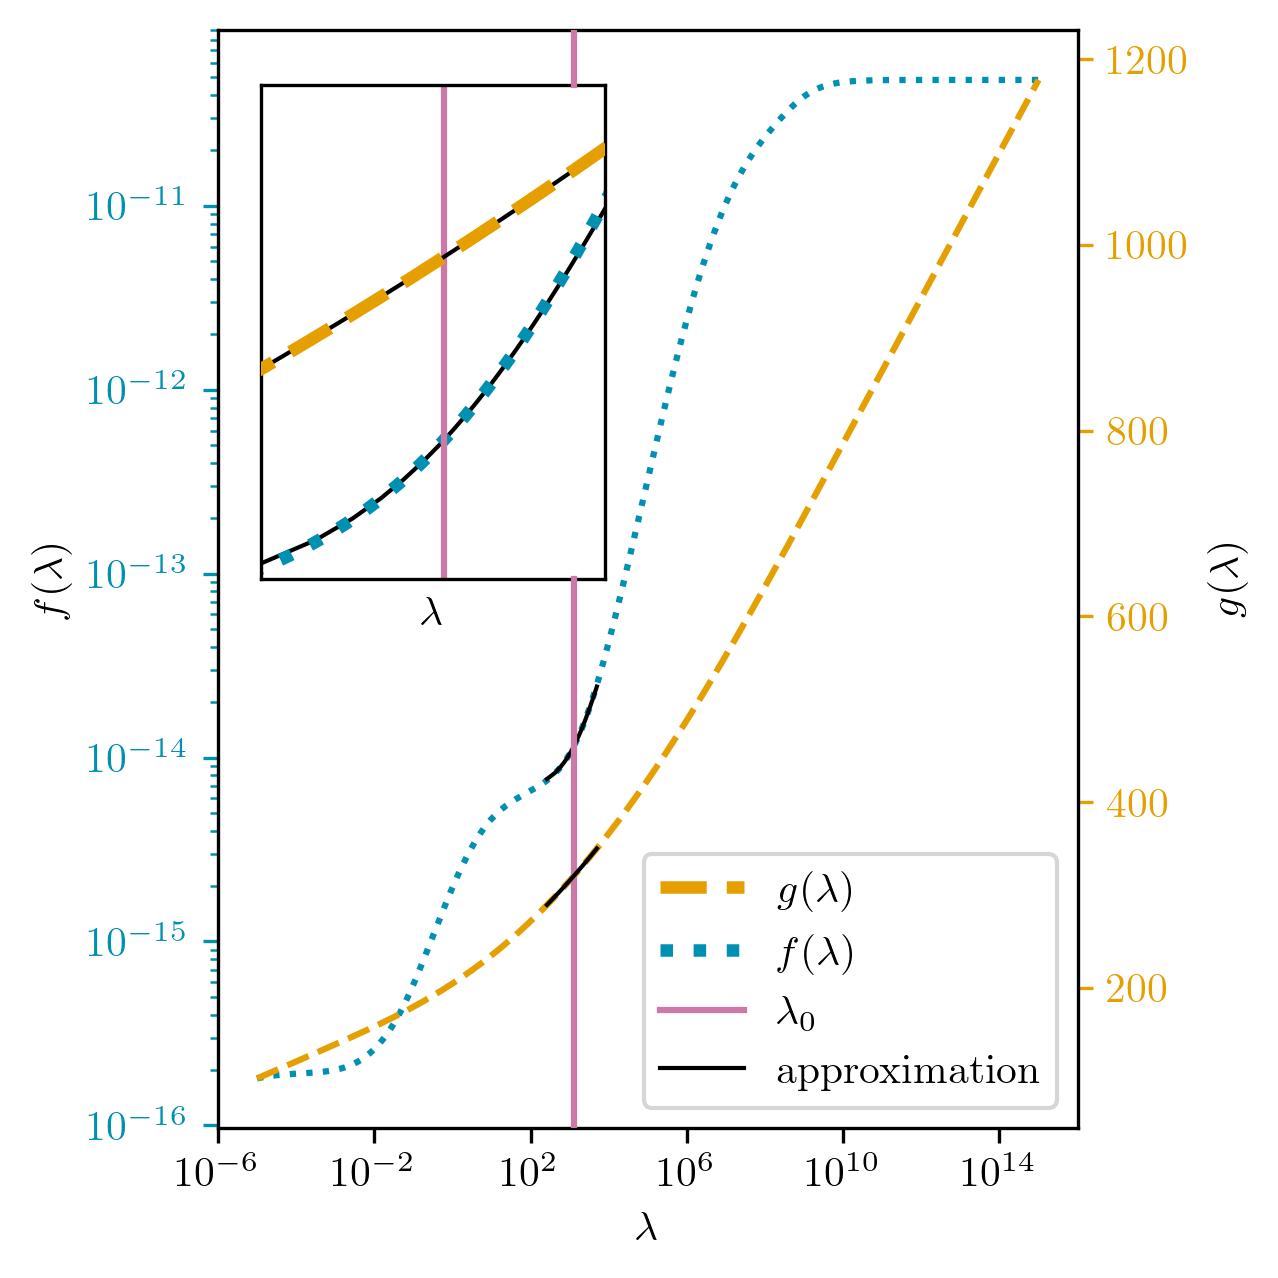
\includegraphics{f_and_g_phd.png}
	\caption[Plot of the functions $f(\lambda)$ and $g(\lambda)$ for marginal posterior.]{Plot of the functions $f(\lambda)$ and $g(\lambda)$ from the marginal posterior for a wide range of $\lambda = \delta / \gamma$. We plot the third order Taylor series in black around the mode of the marginal posterior (vertical line) for the sampling range of $\lambda$ within the MWG algorithm.}
	\label{fig:fandg}
\end{figure}
Most of the computational effort lies in the evaluation of $f(\lambda)$ and $g(\lambda)$, see marginal posterior in Eq. \ref{eq:MargPostAppl}.
In  Fig. \ref{fig:fandg} we see that $f(\lambda)$ and $g(\lambda)$ are well behaved within the region of interest.
Consequently we approximate $f(\lambda) \approx \tilde{f}(\lambda)$ with a 3rd order Taylor series around the mode $\lambda_0$ of $\pi(\lambda, \gamma | \bm{y})$.
We also note that $\tilde{g}(\lambda) \approx g(\lambda)$ behaves linearly around $\lambda_0$ in the log-space.
As a result of these observations, the approximations are implicitly given by
\begin{align}
	f^{(r)}& (\lambda_0)= (-1)^{r+1} r! (\bm{A}^T \bm{y})^T (\bm{B}_0^{-1} \bm{L})^r \bm{B}_0^{-1} \bm{A}_L^T \bm{y} \label{eq:ftay}  \\
	\text{and } & \log{ \tilde{g}(\lambda)} = (\log{\lambda} - \log{\lambda_{0}})  \frac{ \log{g(\lambda_{\text{max}})} - \log{g(\lambda_{0})} }{\log{\lambda_{\text{max}}} - \log{\lambda_{0}} } + \log{ g(\lambda_{0})} 
	\label{eq:gtay}
\end{align} 
with $\bm{B}_0 = \bm{A}^T  \bm{A} + \lambda_0 \bm{L}$.
We plot the approximations in Fig. \ref{fig:fandg} and elaborate on approximation errors in sec \ref{sec:fgErros}






%
%We find the mode at the minimum of  $-\log\{ \pi(\lambda, \gamma | \bm{y}) \}$  using \texttt{scipy.optimize.fmin} function and limit the number of function evaluation to 25 and use Cholesky back and forward substitution to calculate values of $g(\lambda)$ and $f(\lambda)$.
%Additionally, we calculate $\bm{B}_0^{-1} \bm{L} $ and  $\bm{B}_0^{-1}  \bm{A}_L^T \bm{y}$ once more at $\lambda_0$ and plot the Taylor approximation within the sampling region in Fig. \ref{fig:fandg}.



%\subsection{Posterior distributions with Linear model for Ozone -- MTC}
%\label{sec:firstMTC}
%In this section we calculate the posterior marginal and then conditional (MTC) posterior distribution for ozone conditioned on the ground truth temperature and pressure profiles using the linear forward model $\bm{A}_L$.
%This is faster then the other way round (finding temperature over pressure conditioning on ozone) and temperature and pressure are well defined within the atmosphere so it is easier to just condition on a temperature and pressure profile out of a text book.
%We employ a so-called Metropolis within Gibbs (MWG) algorithm on the marginal posterior as summarised in the algorithmic Box \ref{alg:margPost} or use a Tensor-Train (TT) approximation to calculate marginal posterior values.
%Then we can either sample from the conditional posterior using the randomise then optimise (RTO) method or calculate conditional mean and variance using quadrature.


%The DAG in Fig. \ref{fig:DAGO3} visualises that process and we can show explicitly that we group the hyper-parameters $\delta, \gamma$ together to determine the marginal posterior $\pi(\gamma, \delta | \bm{y})$.
%Here $\gamma$ , the noise parameter, determines the noise precision $\bm{\Sigma} = \gamma ^{-1} \bm{I}$ and $\delta$, the smoothness parameter, the precision matrix $\bm{Q} = \delta \bm{L}$ of the prior distribution for $\bm{x}$.
%Then conditioned on the hyper-parameters the conditional posterior $\pi( \bm{x} |\gamma, \delta, \bm{y})$ gives the distribution of posterior ozone profiles.
%Note that we use the linear model $A_L$ here as we do not have an approximation to the non-linear model yet and all prior distributions are defined in Table \ref{tab:priors}.
%The full posterior $\pi(\bm{x},\gamma, \delta | \bm{y}) =  \pi(\bm{x}|\gamma, \delta ,\bm{y}) \pi(\gamma, \delta | \bm{y}) $ is given by multiplication of the marginal and conditional posterior densities. 

%\begin{align}
%	\bm{x} |  \bm{\theta}, \bm{y} \sim \mathcal{N} \Big(
%	\underbrace{\bm{\mu} + \left( \bm{A}^T \bm{\Sigma}^{-1} \bm{A} + \bm{Q} \right)^{-1} \bm{A}^T \bm{\Sigma}^{-1} (\bm{y} - \bm{A} \bm{\mu})}_{\bm{\mu}_{\bm{x} |  \bm{\theta}, \bm{y}}},
%	\underbrace{ \left( \bm{A}^T \bm{\Sigma}^{-1} \bm{A} + \bm{Q} \right)^{-1} }_{\bm{\Sigma}_{\bm{x} |  \bm{y}, \bm{\theta}}}
%	\Big) \, ,
%\end{align}
%is normal distribution and we compute weighted expectations, as in Eq.~\ref{eq:MargExpPos}, of the conditional mean and covariance matrix, where the weights are given by $\pi(\bm{\theta} | \bm{y})$. 
%Note that both the noise covariance $\bm{\Sigma} = \bm{\Sigma}(\bm{\theta})$ and the prior precision matrix $\bm{Q} = \bm{Q}(\bm{\theta})$ depend on the hyper-parameters $\bm{\theta}$.
\subsection{Pressure temperature ratio conditioned on noise and ozone}
\label{subsec:PressTempSetup}
First, we observe that we can describe the pressure values in between $h_{L,0}=7$km and $h_{L,n} = 83.3$km with an exponential function
\begin{align}
	p(h) =
	\exp{ \{ -b \, h  \} } \,  p_0 \quad ,h_{L,n}  \leq h \leq h_{L,0}
	\label{eq:pressFunc}
\end{align}
so that we parametrize the pressure $\bm{p}$ with the hyperparameters $p_0,b$.
Then, within the hierarchical Bayesian framework
\begin{subequations}
	\begin{align}
		\bm{y} |  \bm{p}, \bm{T}, \gamma &\sim \mathcal{N}(\bm{A} \, \bm{p}/\bm{T}, \gamma^{-1} \bm{I}) \label{eq:likelihoodPT} \\
		\bm{a}  &\sim \mathcal{N}(\bm{\mu}_{\bm{a}}, \bm{\Sigma}_{\bm{a}})\\
		\bm{h}_{\bm{T}}  &\sim \mathcal{N}(\bm{\mu}_{\bm{T}}, \bm{\Sigma}_{\bm{h}_T}) \\
		T_0  &\sim \mathcal{N}(\mu_{T_0}, \sigma_{T_0} )\\
		p_0  &\sim \mathcal{N}(\mu_{p_0}, \sigma_{p_0} )\\
		b  &\sim \mathcal{N}(\mu_b, \sigma_b )
	\end{align}
	\label{eq:BayMode}
\end{subequations}
we define a normally distributed likelihood (due to Gaussian noise) and priors, where the hyper-prior means and variances relate to the DAG in Fig. \ref{fig:DAGComplete} so that $\bm{\theta}_{\bm{a}} =(\bm{\mu}_{\bm{a}}, \bm{\Sigma}_{\bm{a}})$, $\bm{\theta}_{\bm{h}_T} = (\bm{\mu}_{\bm{T}}, \bm{\Sigma}_{\bm{h}_T}) $, 
$\bm{\theta}_{T_0} = (\mu_{T_0}, \sigma_{T_0})$, $\bm{\theta}_{p_0} = (\mu_{p_0}, \sigma_{p_0})$, and $\bm{\theta}_{b} = (\mu_{b}, \sigma_{b})$.
Note that we do not include $h_0$, from Tab. \ref{tab:tempGrad}, in $\bm{h}_T$ since we model temperature variability at sea level through $T_0$.

\subsubsection{Prior modelling}
We summarise the mean and variance in Tab. \ref{tab:priors} and plot samples from the prior distribution against the ground truth for the pressure $\bm{p}$ and temperature $\bm{T}$ separately in Fig. \ref{fig:PriorPress} and \ref{fig:PriorTemp} and jointly as $\bm{p}/\bm{T}$ in Fig. \ref{fig:PriorTemp}.
We plot the prior samples against the ground truth for $1/\bm{K}$ in Fig. \ref{fig:OverTempPrior}.
\begin{figure}[ht!]
	\centering
	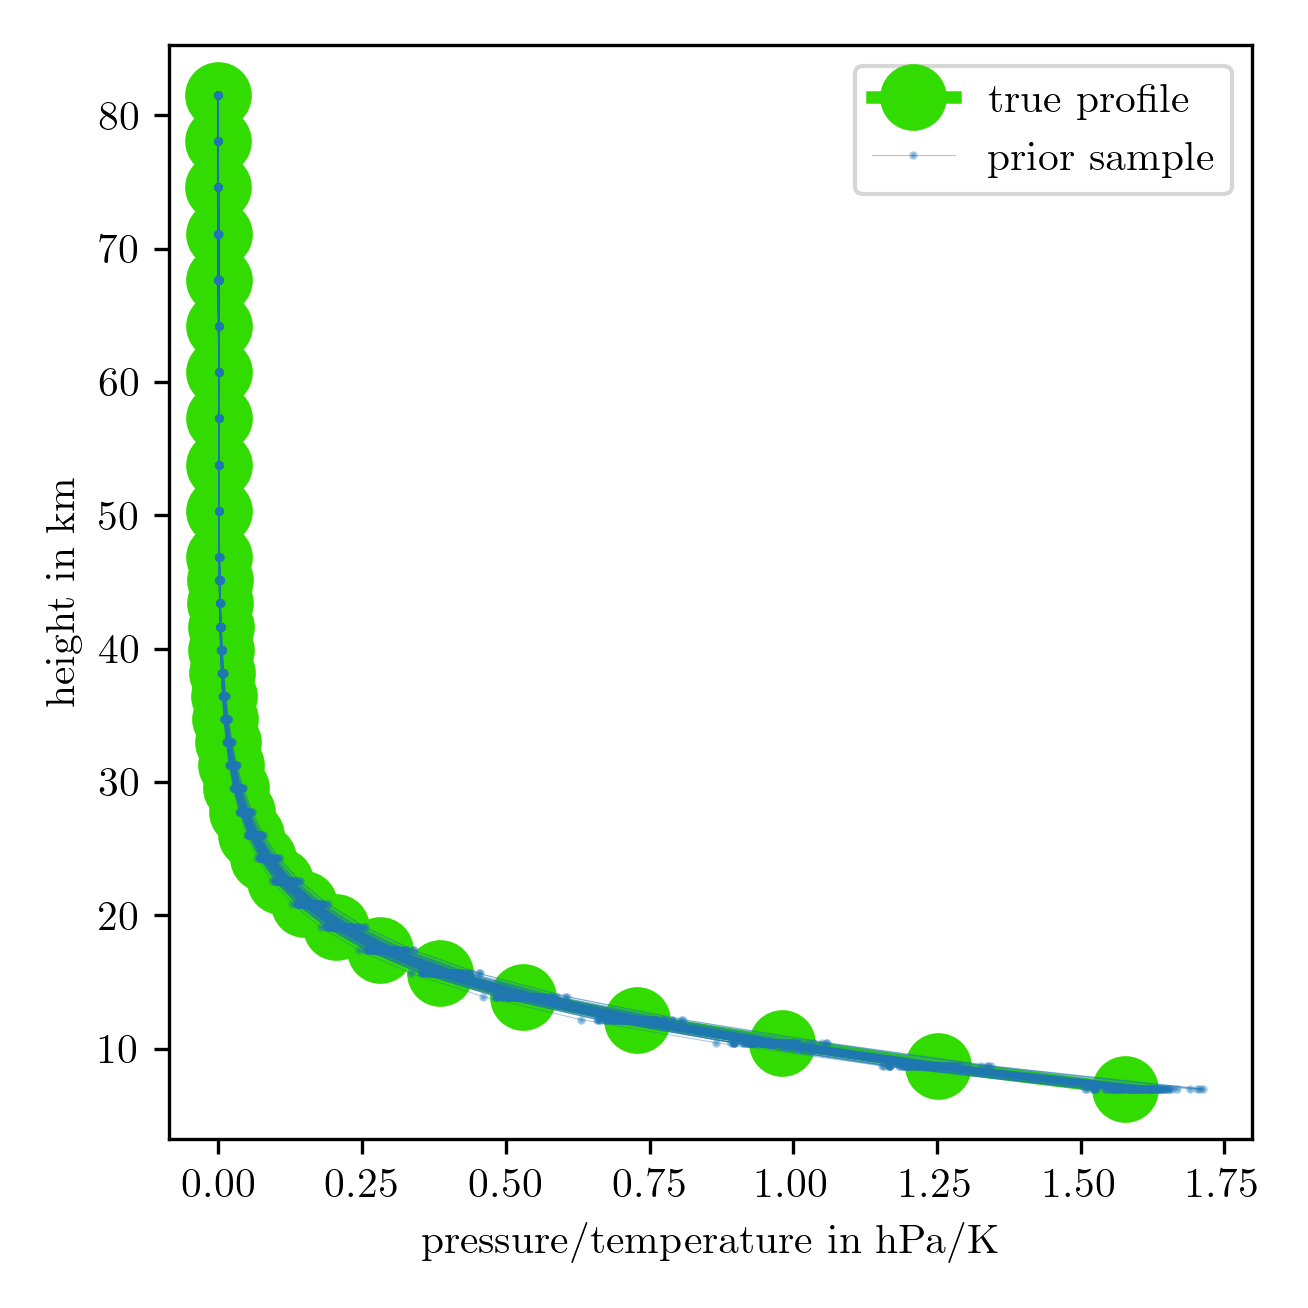
\includegraphics{PriorTempOverPostMeanSigm.png}
	\caption[Prior Samples of $\bm{p}/\bm{T}$ according to the respective hyper-prior distribution.]{We draw samples from the hyper-prior distribution of $h_0, b, p_0, h_1, h_2,h_3,h_4,h_5,h_6, a_0, a_1, a_2,a_3,a_4$ and $T_0$ as defined in table \ref{tab:priors} and then calculate $\bm{p}/\bm{T}$ according to the functions in Eq. \ref{eq:pressFunc} and \ref{eq:tempFunc}.}
	\label{fig:PriorPressOverTemp}
\end{figure}

\begin{figure}[ht!]
	\centering
	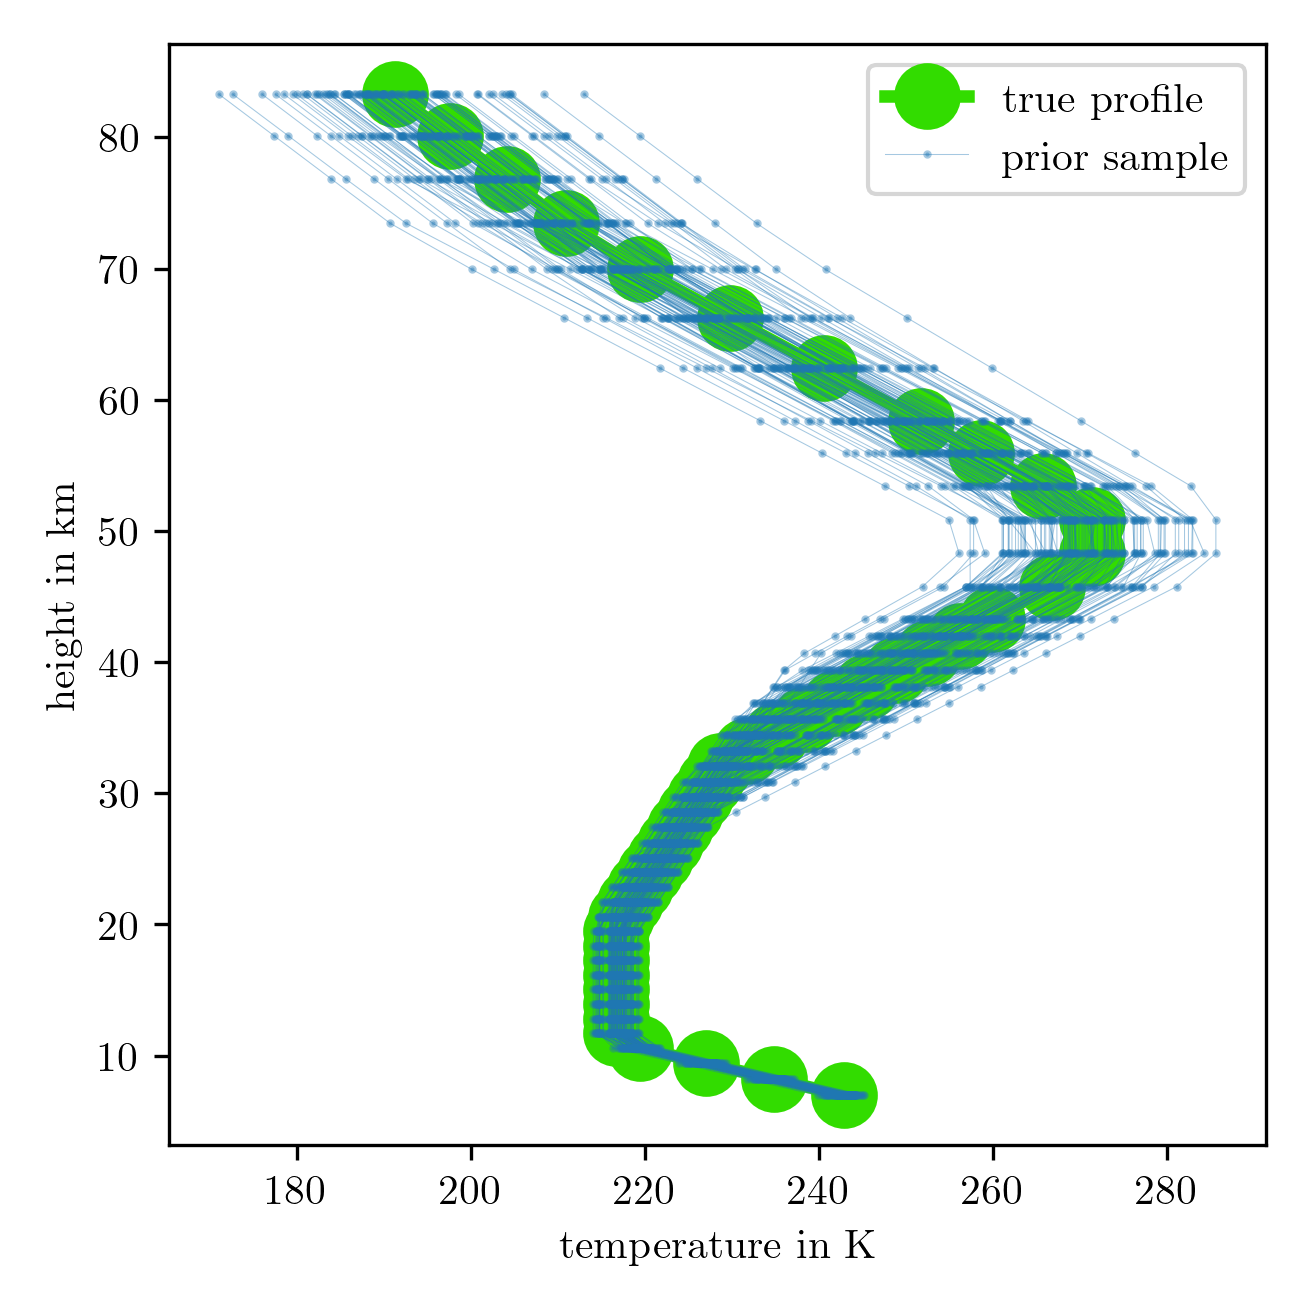
\includegraphics{PriorTempPostMeanSigm.png}
	\caption[Prior Samples of $\bm{T}$ according to the respective hyper-prior distribution.]{We draw samples from the hyper-prior distribution of $h_1, h_2,h_3,h_4,h_5,h_6, a_0, a_1, a_2,a_3,a_4$ and $T_0$ as defined in table \ref{tab:priors} and then calculate $\bm{T}$ according to the function in Eq. \ref{eq:tempFunc}.}
	\label{fig:PriorTemp}
\end{figure}

\begin{figure}[ht!]
	\centering
	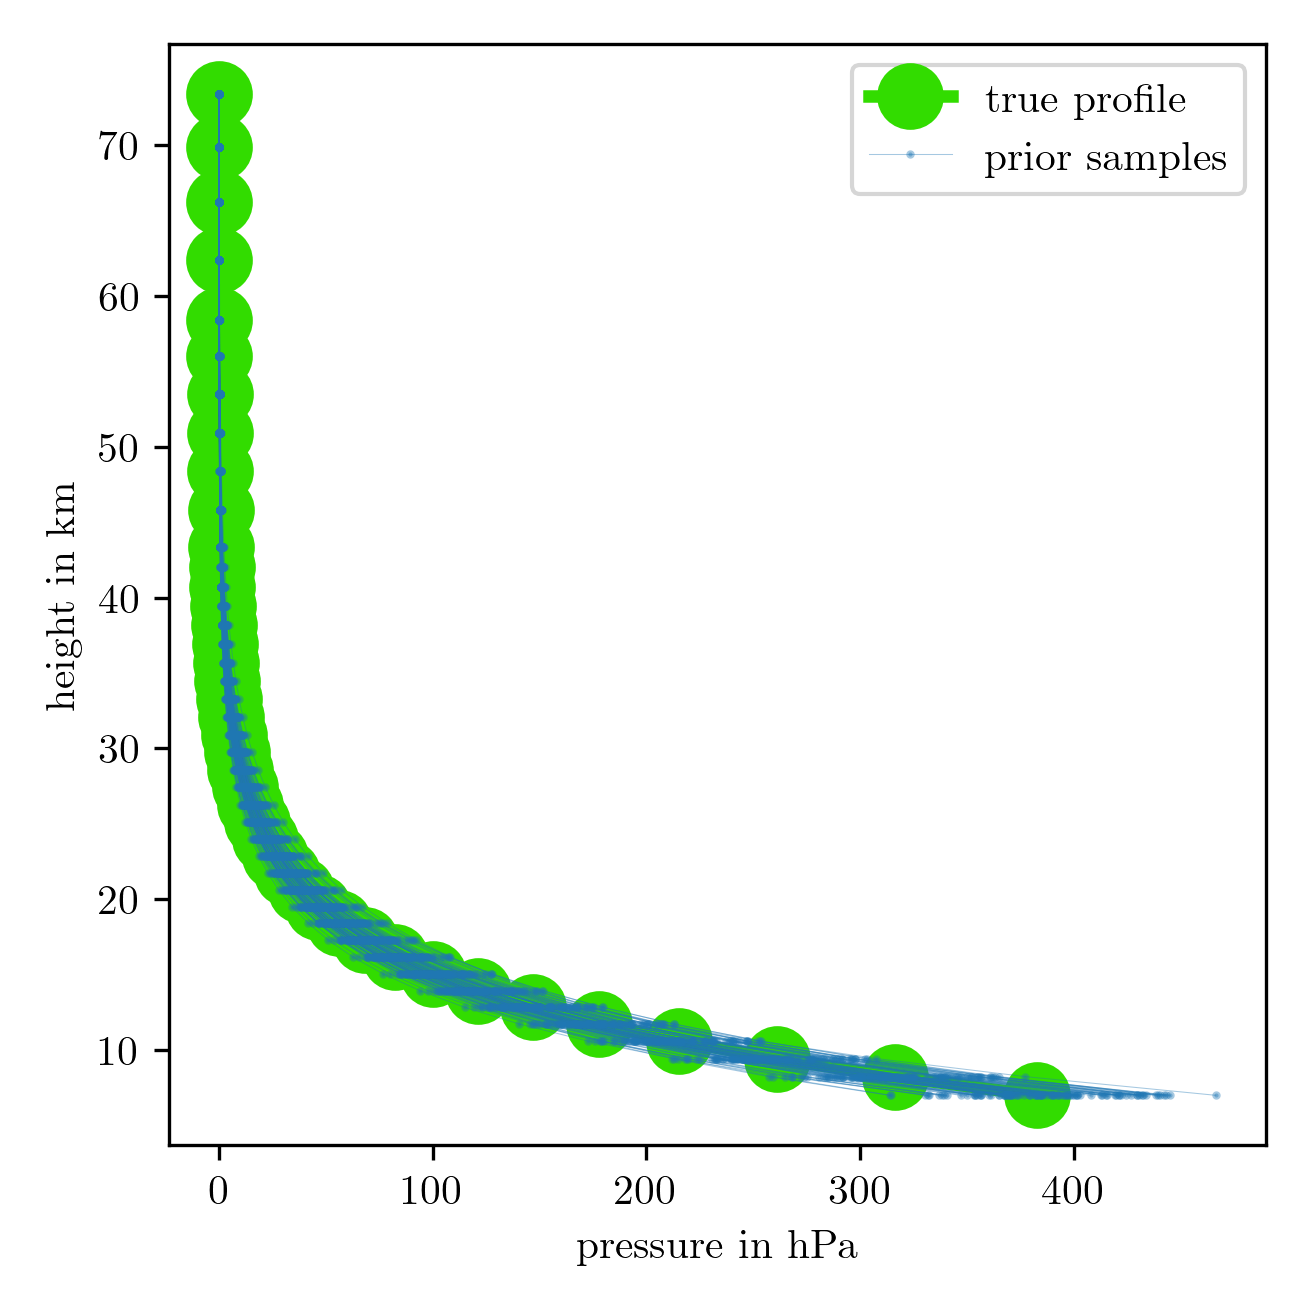
\includegraphics{PriorPressPostMeanSigm.png}
	\caption[Prior Samples of $\bm{p}$ according to the respective hyper-prior distribution.]{We draw samples from the hyper-prior distribution of $h_0, b$ and $p_0$ as defined in table \ref{tab:priors} and then calculate $\bm{p}$ according to the function in Eq. \ref{eq:pressFunc}.}
	\label{fig:PriorPress}
\end{figure}


We carefully choose the hyper-prior distributions $\bm{h}_{\bm{T}} $ so that the individal distributions for heights $h_1, h_2, h_3, h_4,h_5,h_6$ do not overlap, see Fig. \ref{fig:HeightPriors}.
Additionally, we define the sampling space and the grid for the TT approximation accordingly.
We remark that we can already observe in Fig. \ref{fig:PriorPressOverTemp} that $\bm{p}/\bm{T}$ inherits the structure of the pressure function.

\subsubsection{posterior distribution}
Then we can define the posterior distribution
\begin{align}
		\pi(p_0,b,\bm{h_T},\bm{c_T},\bm{a_T} | \bm{y}, \gamma, \bm{x}) \propto  \exp\Bigl\{ & -\frac{\gamma}{2} \left\Vert \bm{y}- \bm{A} \frac{\bm{p}}{\bm{T}}  \right\Vert^2 \Bigr\} \pi(p_0,b,\bm{h_T},\bm{c_T},\bm{a_T})\, ,
\end{align}
which is, conditioned on the noise hyper-parameter $\gamma$, the ozone profile $\bm{x}$ and the smoothness hyper-parameter $\delta$, a 16 dimesnional distribution.
\clearpage


\section{Approximate non-linear forward model with affine Map} 
\label{sec:affineMap}
With the posterior distributions formulated, we can now approximate the non-linear forward model with an affine map $\bm{M}$; we see Fig. \ref{fig:affinStrat} for the summarised strategy.
We focus on the posterior distribution of ozone profiles by conditioning on pressure and temperature, as this is a quick process when using the MTC method.
We approximate and sample from the marginal posterior $ \pi(\gamma , \delta|\bm{y})$ and then characterise the full conditional posterior distribution $\pi(\bm{x}|\bm{y})$ based on the linear forward model $\bm{A}_L$, neglecting absorption, see Eq. \ref{eq:RTE}.
Given samples $\bm{x} \sim \pi(\bm{x}|\bm{y})$ from the full conditional posterior distribution, we can generate two affine subspaces based on the linear and non-linear model and find the mapping between those.

\begin{figure}[htb!]
	\centering
	\begin{tikzpicture}
		\node[rectnode] at (0,0) (Oy)    {$\bm{y}$};
		\node[roundnode2] at (0,-2) (x)     {$\bm{x}$};
		\node[rectnode] at (-1.75,-4) (NLy)    {$\bm{A}_{NL}\bm{x}$};
		\node[rectnode] at (1.75,-4) (y)    {$\bm{A}_L\bm{x}$};
		\draw[->, very thick] (Oy.south) -- (x.north); 
		\draw[->, very thick] (x.south west) -- (NLy.north); 
		\draw[->, very thick] (x.south east) -- (y.north); 
		\draw[->, very thick] (NLy.east) -- (y.west); 
		\node[align=center] at (1,0) (l1) {Data};
		\node[align=center] at (3.5,-2) (f2) {Ozone Profiles from $\pi(\bm{x}|\gamma, \lambda ,\bm{y}) $};
		\node[align=center] at (1.75,-1) (l1) {$\pi(\lambda , \gamma  | \bm{y})$ with $\bm{A}_L$};
		
		\node[align=center] at (-4.75,-4) (f3) {non-linear forward model};
		\node[align=center] at (4.25,-4) (f4) {linear forward model};
		\node[align=center] at (0,-5) (f5) {$\bm{A}_{NL} \approx \bm{M A}_L= \bm{A}$ };
		
		\node[align=center] at (0,-4) (f5) {affine Map \\ $\bm{M}$};
		
	\end{tikzpicture}
	\caption[Strategy to find affine map.]{The strategy to find the affine map consist of evaluating the marginal posterior for ozone using the linear forward model. Then we draw ozone samples from the conditional posterior and calculate noise free data based on the linear and non-linear forward model. Next we find a mapping in between those two space so that we can approximate the non-linear forward model using an affine map and the linear forward model.}
	\label{fig:affinStrat}
\end{figure}


\subsection{Sample from marginal posterior distribution for ozone}
\label{subsec:firstMarg}
We set $\bm{A} = \bm{A}_L$ and characterise the marginal posterior $\pi(\lambda, \gamma | \bm{y})$ as in Eq. \ref{eq:MargPostAppl} by employing a Metropolis within Gibbs (MWG) algorithm, see sec. \ref{}.
More specifically, we implement a Metropolis random walk on the full conditional
\begin{align}
	\label{eq:lamCondPrior}
	\pi(\lambda | \gamma, \bm{y}) &\propto \lambda^{n/2+\alpha_\delta -1} \exp{\Bigl\{ - \frac{1}{2} g ( \lambda) - \frac{\gamma}{2} f ( \lambda) - \beta_\delta \gamma \lambda \Bigr\}} 
\end{align} 
and do a Gibbs step on
\begin{align}
	\gamma |  \lambda, \bm{y} &\sim \Gamma \bigg( \frac{m}{2} + \alpha_\delta + \alpha_\gamma, \frac{1}{2} f (\lambda ) + \beta_\gamma + \beta_\delta \lambda \bigg)\label{eq:GibbsStep}
\end{align} 
to generate marginal posterior samples $(\lambda, \gamma)^{(1)}, \dots, (\lambda, \gamma)^{(N)} \sim  \pi(\lambda, \gamma| \bm{y})$.
Note that, when changing variables from $\delta = \lambda \gamma$ to $\lambda$ the hyper-prior distribution changes to $\pi(\lambda) \propto \lambda^{\alpha_\delta-1} \gamma^{\alpha_\delta} \exp{(- \beta_\delta \lambda  \gamma)} $, due to $\text{d}\delta / \text{d} \lambda = \gamma$.

Hence we run a Metropolis random walk on $\pi(\lambda | \gamma, \bm{y})$, the proposal distribution $q(\lambda^\prime|\lambda^{(k)}) \sim \mathcal{N}(\lambda^{(k)}, 0.8 \lambda_{0})$ conditioned on the previous sample $\lambda^{(k)}$, with $k = 1 , \dots, N$ is symmetric.
Then, we accept or reject a new $\lambda^{\prime}$ sample by comparing the acceptance ratio
\begin{align} 
	\log \left\{ \frac{\pi(\lambda^{\prime} | \gamma^{(k)}, \bm{y})  }{\pi(\lambda^{(k)}| \gamma^{(k)}, \bm{y})}  \right\} 
	= \log  \{\pi(\lambda^{\prime} | \gamma^{(k)}, \bm{y} ) \}  -\log  \{ \pi(\lambda^{(k)}| \gamma^{(k)}, \bm{y}) \} \\
	= \frac{n}{2} (\log\{\lambda^{\prime}\} - \log\{\lambda^{(t-1)}\} ) + \frac{1}{2} \Delta g + \frac{\gamma^{(t-1)}}{2} \Delta f  + \beta_\delta \gamma^{(t-1)} \Delta \lambda  \, ,
\end{align}
where $\Delta \lambda = \lambda^{\prime} - \lambda^{(k)} $ to a random uniform number in between 0 and 1.
Note that since we calculate the acceptance ratio in the log space $\Delta f \approx \tilde{f}(\lambda^\prime) - \tilde{f}(\lambda^{(k)}) = \sum f^{(r)} (\lambda_0)\Delta \lambda^\prime - \Delta \lambda^{(k)} $ is a 3rd order taylor approximaton, see Fig. \ref{fig:fandg}, where $\Delta \lambda^{\prime} = \lambda^\prime - \lambda_0 $ and $\Delta \lambda^{(k)} =  \lambda^{(k)} - \lambda_0$.
Similarly we approximate $\Delta g \approx \exp{\log{\tilde{g}(\lambda^{\prime})}} - \exp{\log{\tilde{g}(\lambda^{(k)})}}$ as in Eq. \ref{eq:fandg}.
Lastly, a Gibbs step provides a new $\gamma^{(k+1)} \sim \gamma | \lambda^{(k+1)}, \bm{y}$, see Equation \eqref{eq:GibbsStep}.
See Algorithmic Box \ref{alg:margPost} for a summary of the general version.

We initialise the MWG at the mode $( \lambda^{(0)} , \gamma^{(0)}  ) = ( \lambda_{0} , \gamma_{0}  )$ and take for $N = 10000$ plus $N_{\text{burn-in}} = 100$ steps in less than $0.3$s.
The standard deviation of the normal proposal distribution is set to $\sigma_{\lambda} = 0.8 \lambda_0$ so that the acceptance rate is $\approx 0.5$ as suggested in \cite{}.
The samples are plotted in Fig. \ref{fig:ScatterPlotTT} as a 2D scatter plot, as well as the trace of the MwG to show ergodicity.
We calculate the integrated autocorrelation time (IACT) with the Python implementation of \cite{}, which gives us $\tau_{\text{int}, \gamma} = $ and $\tau_{\text{int}, \delta} = $.


\begin{figure}[ht!]
	\centering
	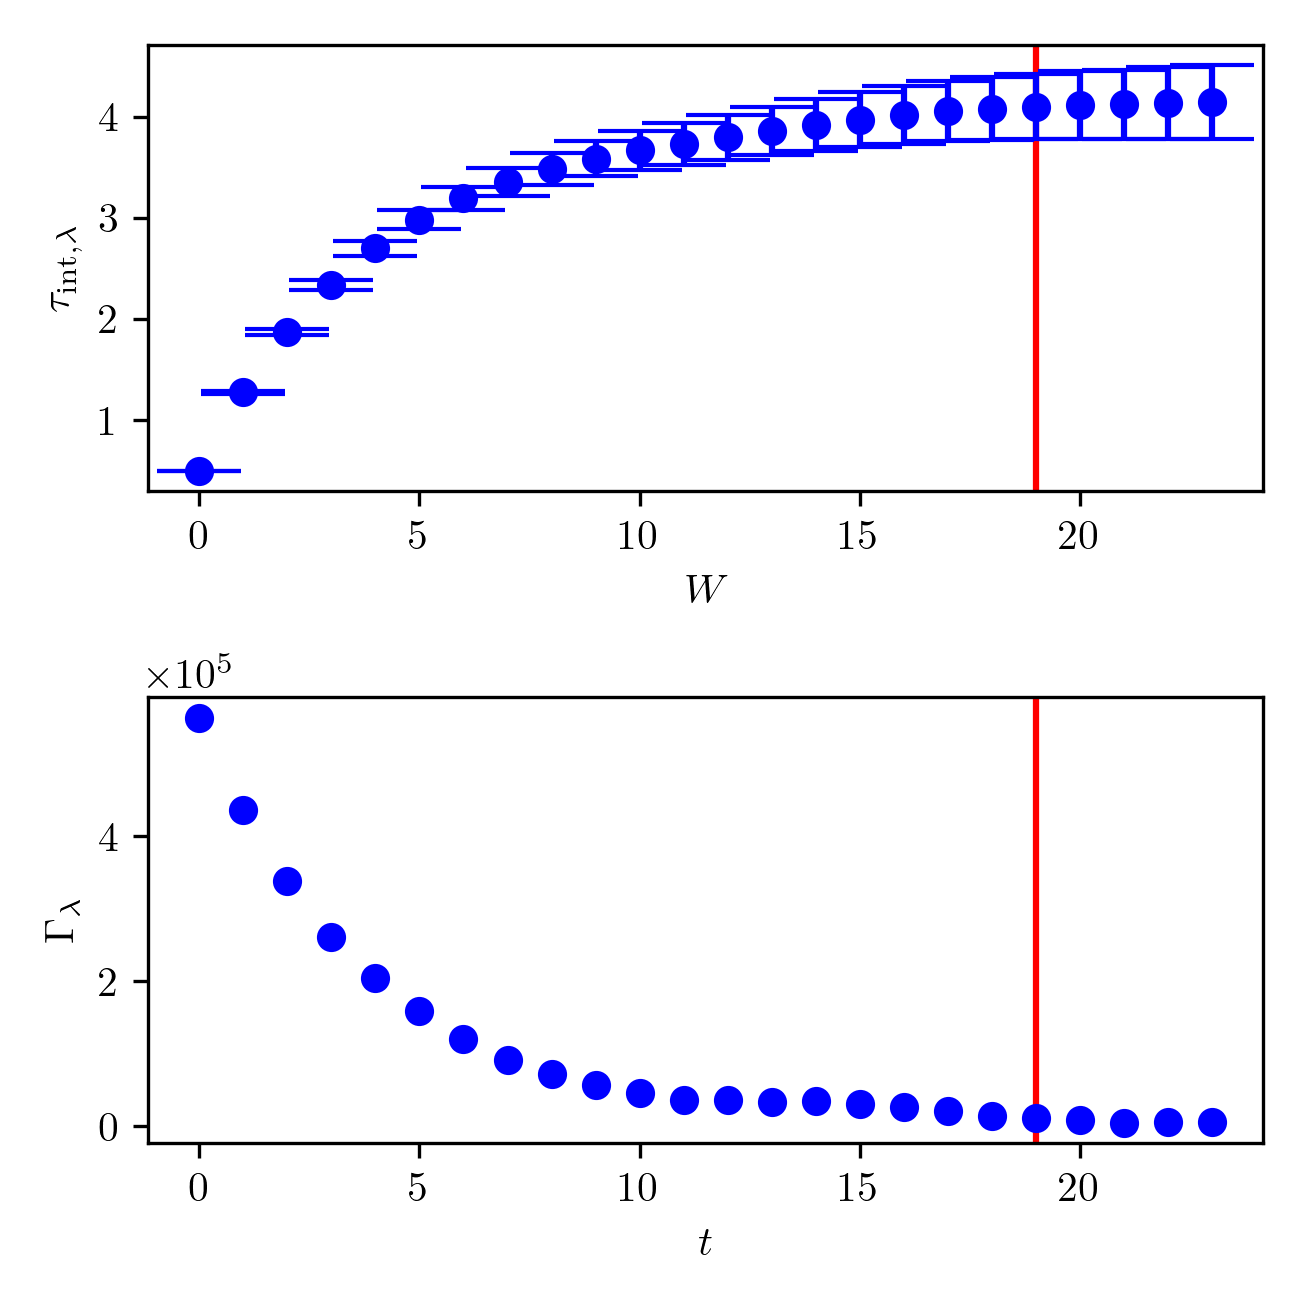
\includegraphics{UwerrTauIntFirstO3lam.png}
	\caption[]{}
	\label{fig:}
\end{figure}
\begin{figure}[ht!]
	\centering
	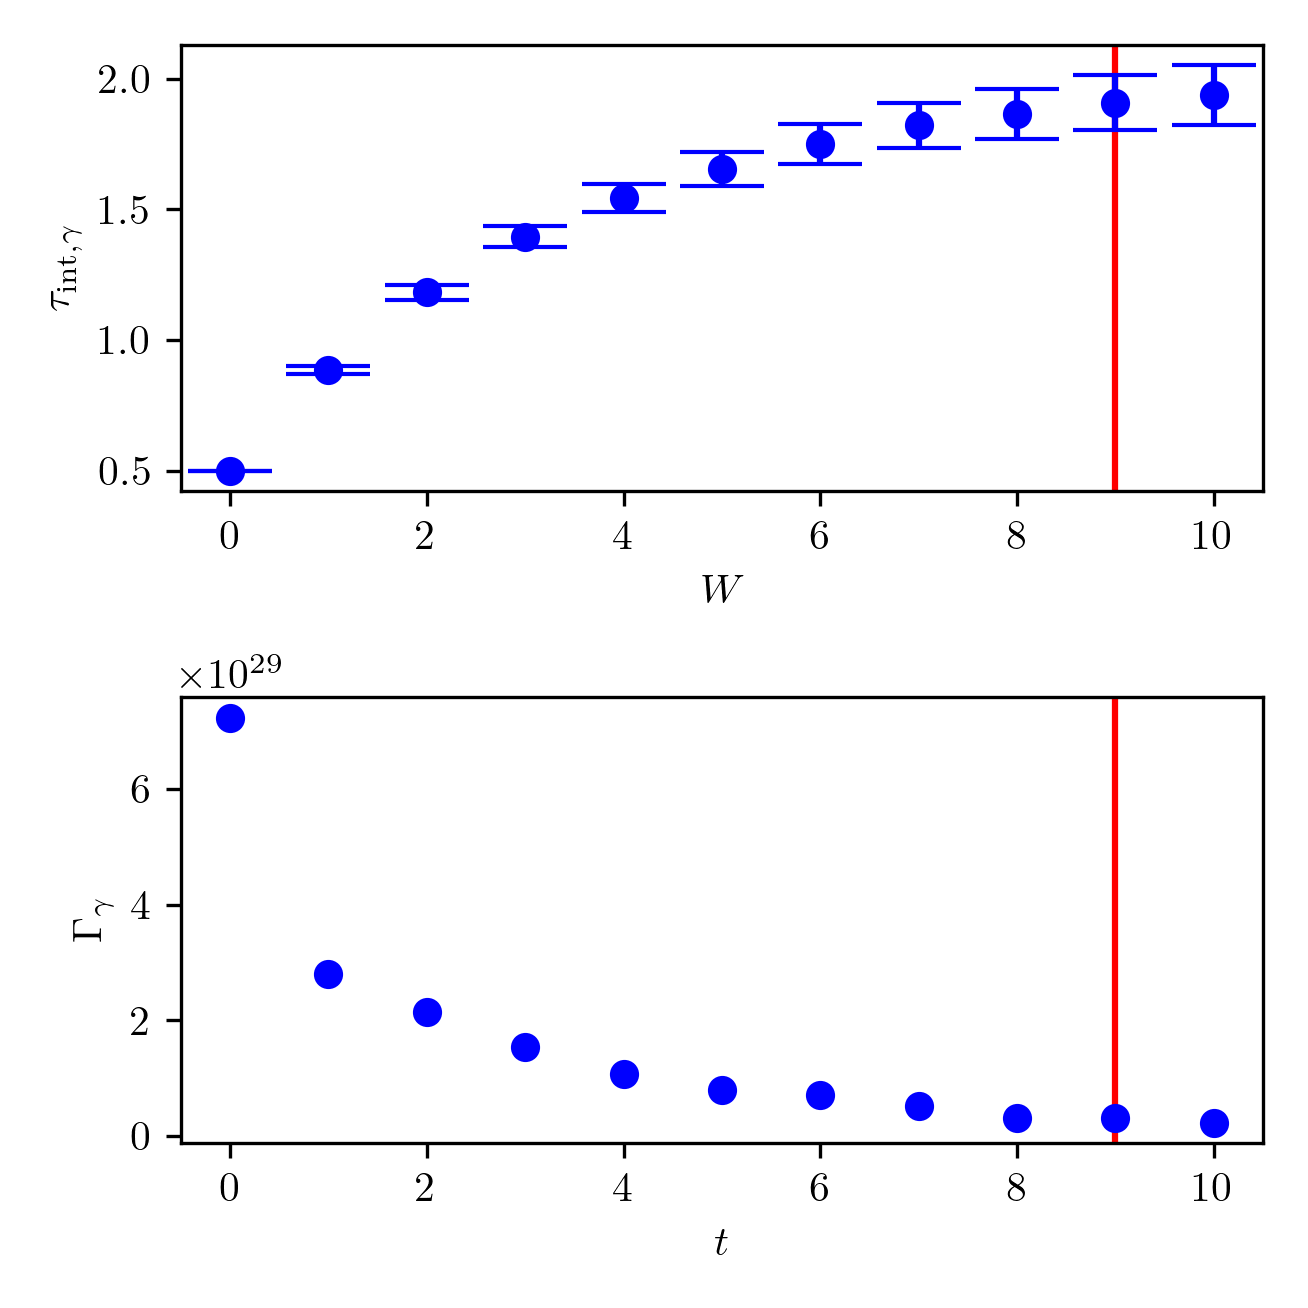
\includegraphics{UwerrTauIntFirstO3gam.png}
	\caption[]{}
	\label{fig:}
\end{figure}

%\begin{algorithm}[!ht]
%	\caption{Metropolis within Gibbs for $\pi(\lambda, \gamma | \bm{y})$}
%	\begin{algorithmic}[1]
%		\STATE Initialise  \( \bm{\theta}^{(0)}  =( \lambda^{(0)} , \gamma^{(0)}  ) \) and set burn-in $N_{\text{burn-in}}$
%		\FOR{ \( k = 1, \dots, N^{\prime} \)}
%		\STATE Propose \( \lambda \sim \mathcal{N}(\lambda^{(t-1)}, 0.8 \lambda_0)  \)
%		\STATE Compute
%		\[ \alpha( \lambda  | \lambda^{(t-1)}) = \min \left\{ 1, \frac{\pi(\lambda | \gamma^{(t-1)}, \bm{y})  }{\pi(\lambda^{(t-1)}| \gamma^{(t-1)}, \bm{y})}  \right\} \]
%		\STATE Draw $u \sim \mathcal{U}(0,1)$
%		\IF{$\alpha \geq u$ }
%		\STATE Accept and set \( \lambda^{(t)} = \lambda \)
%		\ELSE  
%		\STATE Reject and keep \(\lambda^{(t)} = \lambda^{(t-1)} \)
%		\ENDIF
%		\STATE Draw $\gamma^{(t)} | \lambda^{(t)} ,\bm{y} \sim \text{Gamma} \big( 0.5  \, m + 2, 0.5 \, f(\lambda^{(t)}) + 10^{-10}(1 + \lambda^{(t)}) \big) $
%		\ENDFOR
%		%\STATE Output: $ \bm{\theta}^{(N_{\text{burn-in}})}, \dots,  \bm{\theta}^{(k)} , \dots,   \bm{\theta}^{(N)} \sim \pi(\bm{\theta}| \bm{y}) $
%		\STATE Output: $ (\lambda, \gamma)^{(N_{\text{burn-in}})}, \dots,  (\lambda, \gamma)^{(k)} , \dots,   (\lambda, \gamma)^{(N)} \sim \pi(\lambda, \gamma| \bm{y}) $
%	\end{algorithmic}
%	\label{alg:margPost}
%\end{algorithm}

\subsection{Tensor-train approximation of the marginal posterior distribution for ozone}
\label{sec:firstMargTT}
Alternatively, we can approximate the marginal posterior with a tensor-train (TT) of the square root of the marginal posterior on a predefined grid.
We define a grid similar to the sampling region of the MWG sampler with 25 grid points in each dimension and use the \texttt{tt.cross.rectcross.rect\_cross.cross} function from the \texttt{ttpy} Python package, based on the rect cross algorithm in \cite{}.
We set the number of ranks to a constant value $r = 4$ and optimise over those ranks with one sweep to calculate the cores in less than $0.1$s.
To avoid underflow, we have to add a 'normalisation' constant $c = 460$ so that we approximate $\pi(\lambda | \gamma ,\bm{y}) = \exp\{ \log{\pi(\lambda | \gamma, \bm{y})} + c\}$.
Then we calculate the marginals $\pi(\lambda| \bm{y})$ and $\pi(\gamma| \bm{y})$ as described in section \ref{}, assuming an absolute error of $1$ the constant $\xi = 1/ \uplambda(\mathcal{X}) $, with a diagonal mass matrix $\bm{M}_k=  \text{diag}(\uplambda(X_k))$, where $\uplambda(X_k)$ is the length of the grid of the $k$th dimension also knows as the Lebesgue measure of a closed interval.
We plot the TT approximation as a colour map on top of the obtained samples in the scatter plot in Fig. \ref{fig:ScatterPlotTT}.
\begin{figure}[ht!]
	\centering
	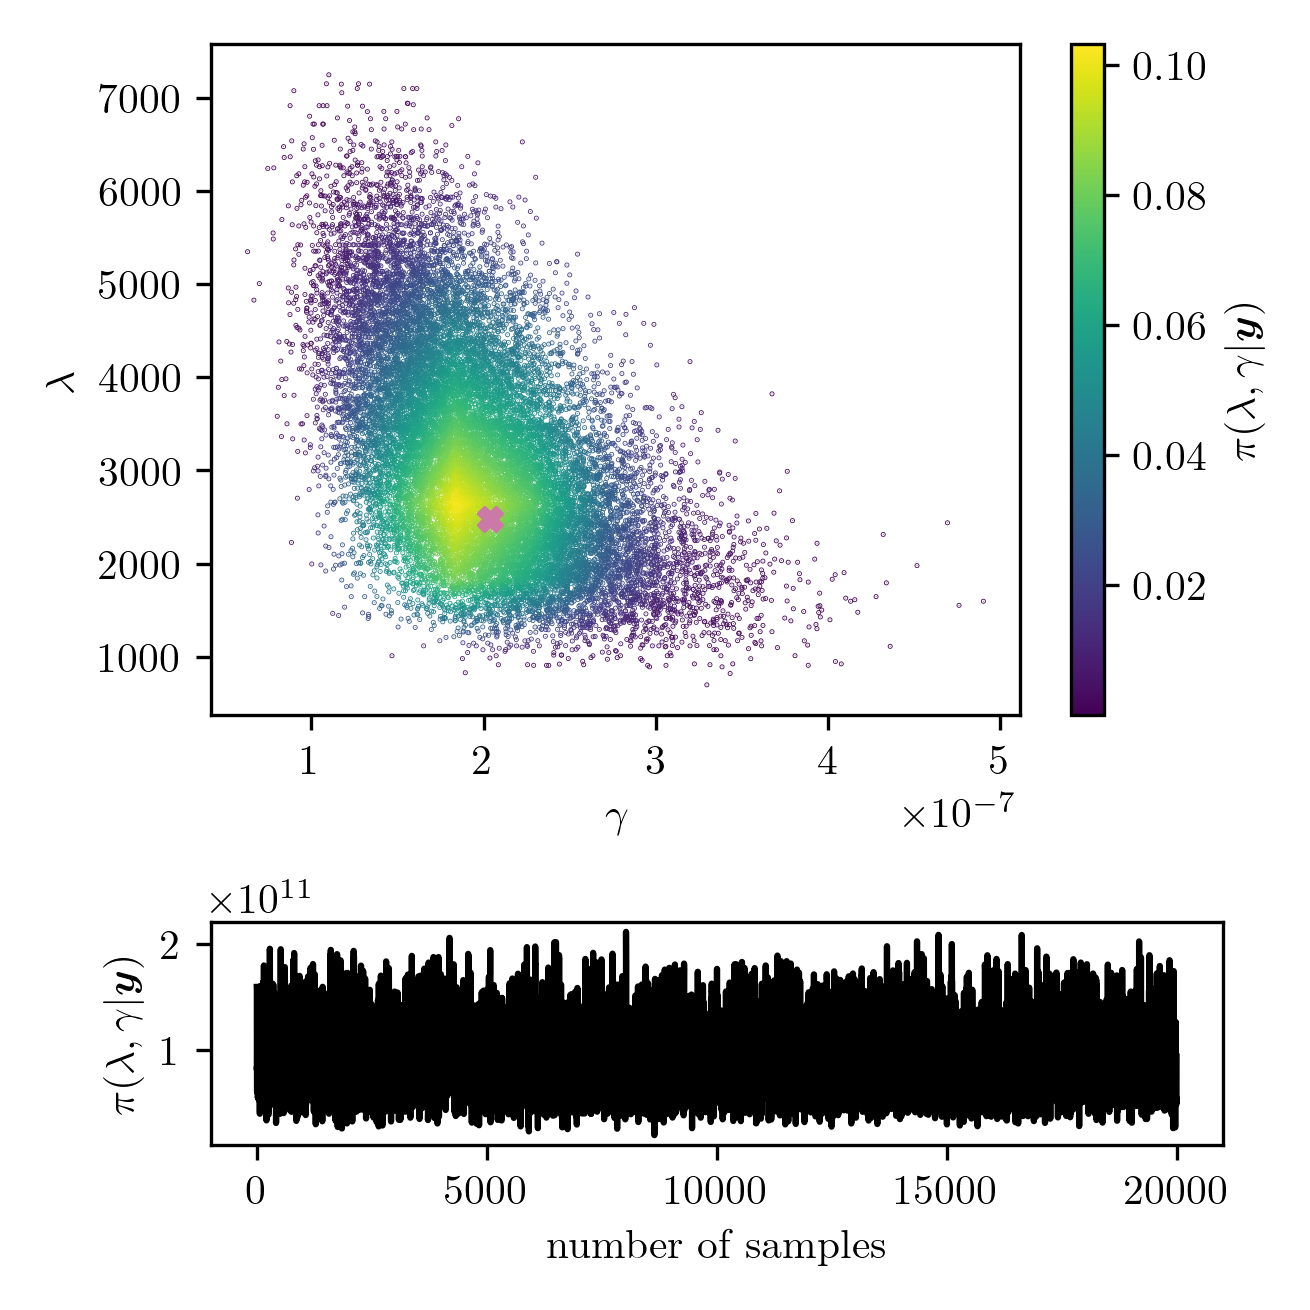
\includegraphics{ScatterplusHistoPlusTT.png}
	\caption[Scatter plot of samples from marginal posterior, including weighting from TT approximation; additional trace plot of the marginal posterior samples.]{We scatter plot the samples of $\lambda = \delta / \gamma $ and $\gamma$ from the marginal posterior $\pi(\lambda , \gamma  | \bm{y})$ and colour code the samples using the TT approximation of $\pi(\lambda , \gamma  | \bm{y})$. The mode of $(\lambda_0 , \gamma_0)$ of $\pi(\lambda , \gamma  | \bm{y})$ provided by \texttt{scipy.optimize.fmin} is marked with the cross. To show ergodicity we plot the trace of the samples of the Metropolis-within-Gibbs sampler below.}
	\label{fig:ScatterPlotTT}
\end{figure}

\begin{figure}[ht!]
	\centering
	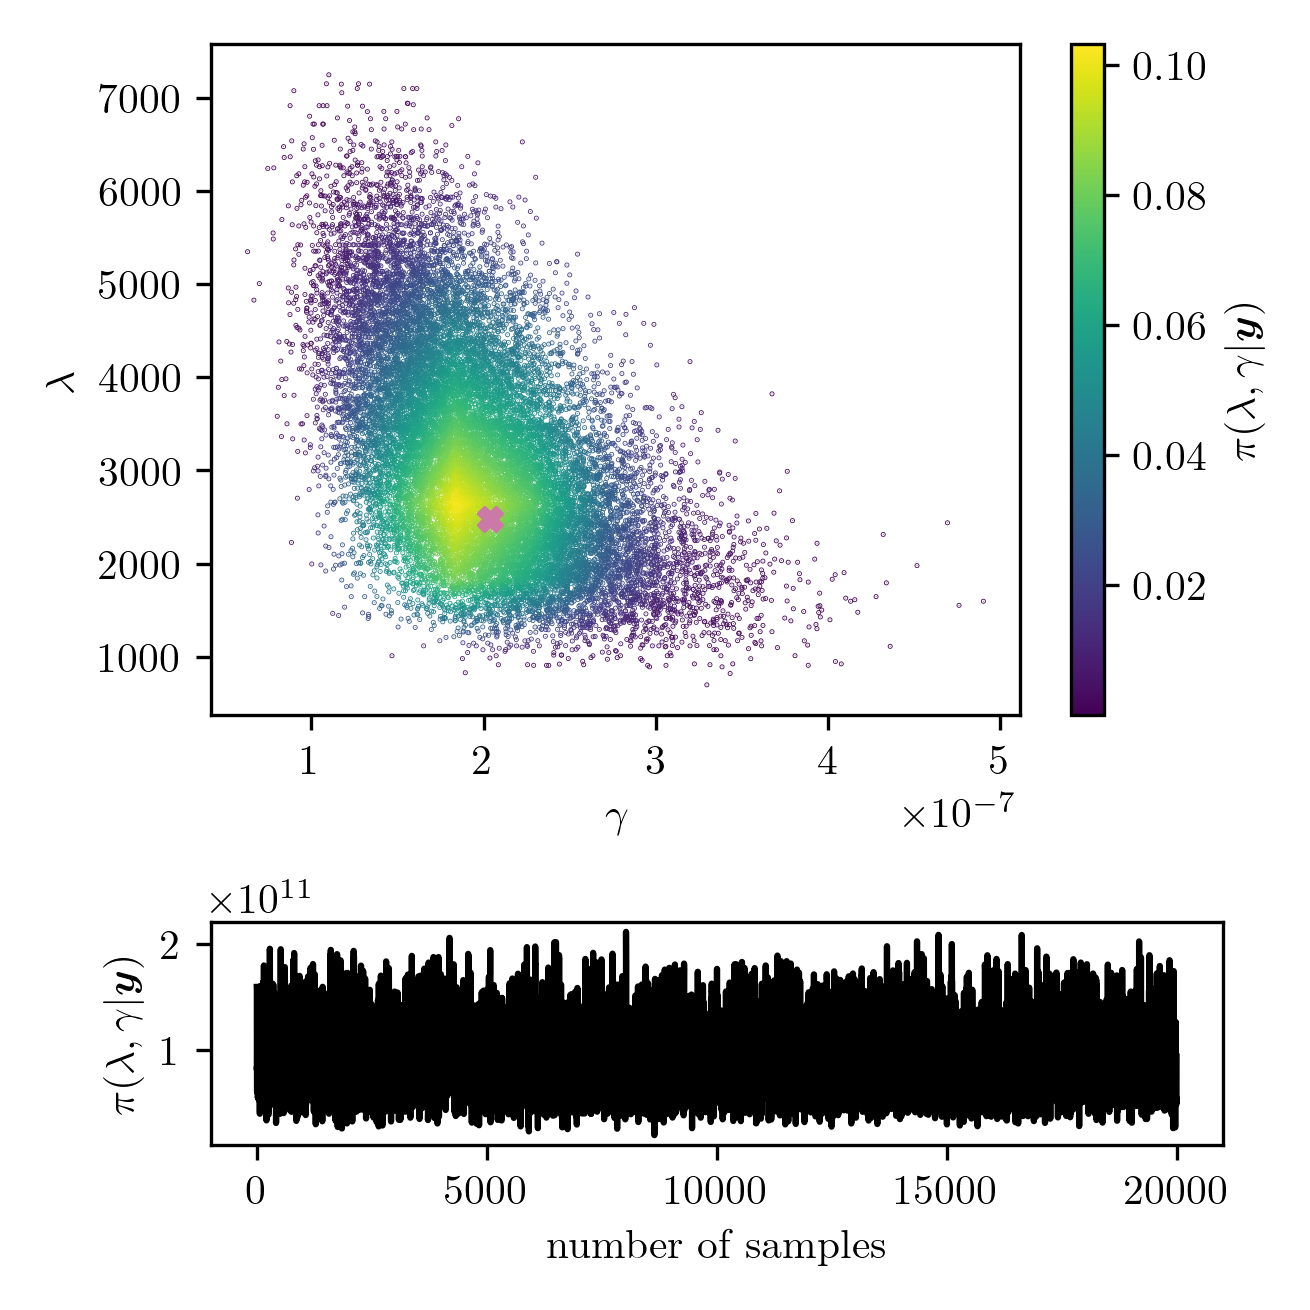
\includegraphics{ScatterplusHistoPlusTT.png}
	\caption[]{}
	\label{fig:UwerrMargFirst}
\end{figure}



\subsection{Calculate mean and variance of the full conditional posterior for ozone}
\label{subsec:firstCond}
Based on the marginal posteror distribution $\pi(\gamma, \delta | \bm{y})$ we calculate the weighted mean and covariance of the conditional posterior $\pi(\bm{x} | \gamma, \delta, \bm{y})$ by quadrature as in Eq. \ref{eq:MeanInt} and Eq. \ref{eq:CovInt}.

By binning the output samples from the MWG, see Fig. \ref{fig:ScatterPlotTT}, into a normalised histogram with 25 bins, we obtain function values for the marginal posterior.
With the height of the histogram bars as quadrature weights, e.g. $\pi(\lambda_i| \bm{y})$, where $\lambda_i$ is the centre of each bin we calculate the full conditional mean $\bm{\mu}_{\bm{x}|\bm{y}}$ and covariance matrix $\bm{\Sigma}_{\bm{x}|\bm{y}}$ as weighted expectations.

Alternatively we use the marginal distributions $\pi(\delta | \bm{y})$ and $\pi(\gamma | \bm{y})$ from the TT approximation of $\sqrt{\pi(\delta, \gamma | \bm{y})}$ to calculate 
weighted expectations of $\bm{\mu}_{\bm{x}|\bm{y}}$ and $\bm{\Sigma}_{\bm{x}|\bm{y}}$.

In practice, we have to invert $\bm{B}_{\lambda} $ and calculate $\bm{x}_{\lambda}$, see Eq. \ref{eq:CondPost} 25 times (TT grid size and number of bins).
A feasible method is the Cholesky forward and backwards substitution \cite{}, which takes roughly $1$s to compute the mean and variance.
Note that we reject unphysical samples from the conditional posterior with negative ozone values and plot those in Fig. \ref{fig:O3Samp}, including variance and mean.

Computation time is less than $0.2$s.
\begin{figure}[ht!]
	\centering
	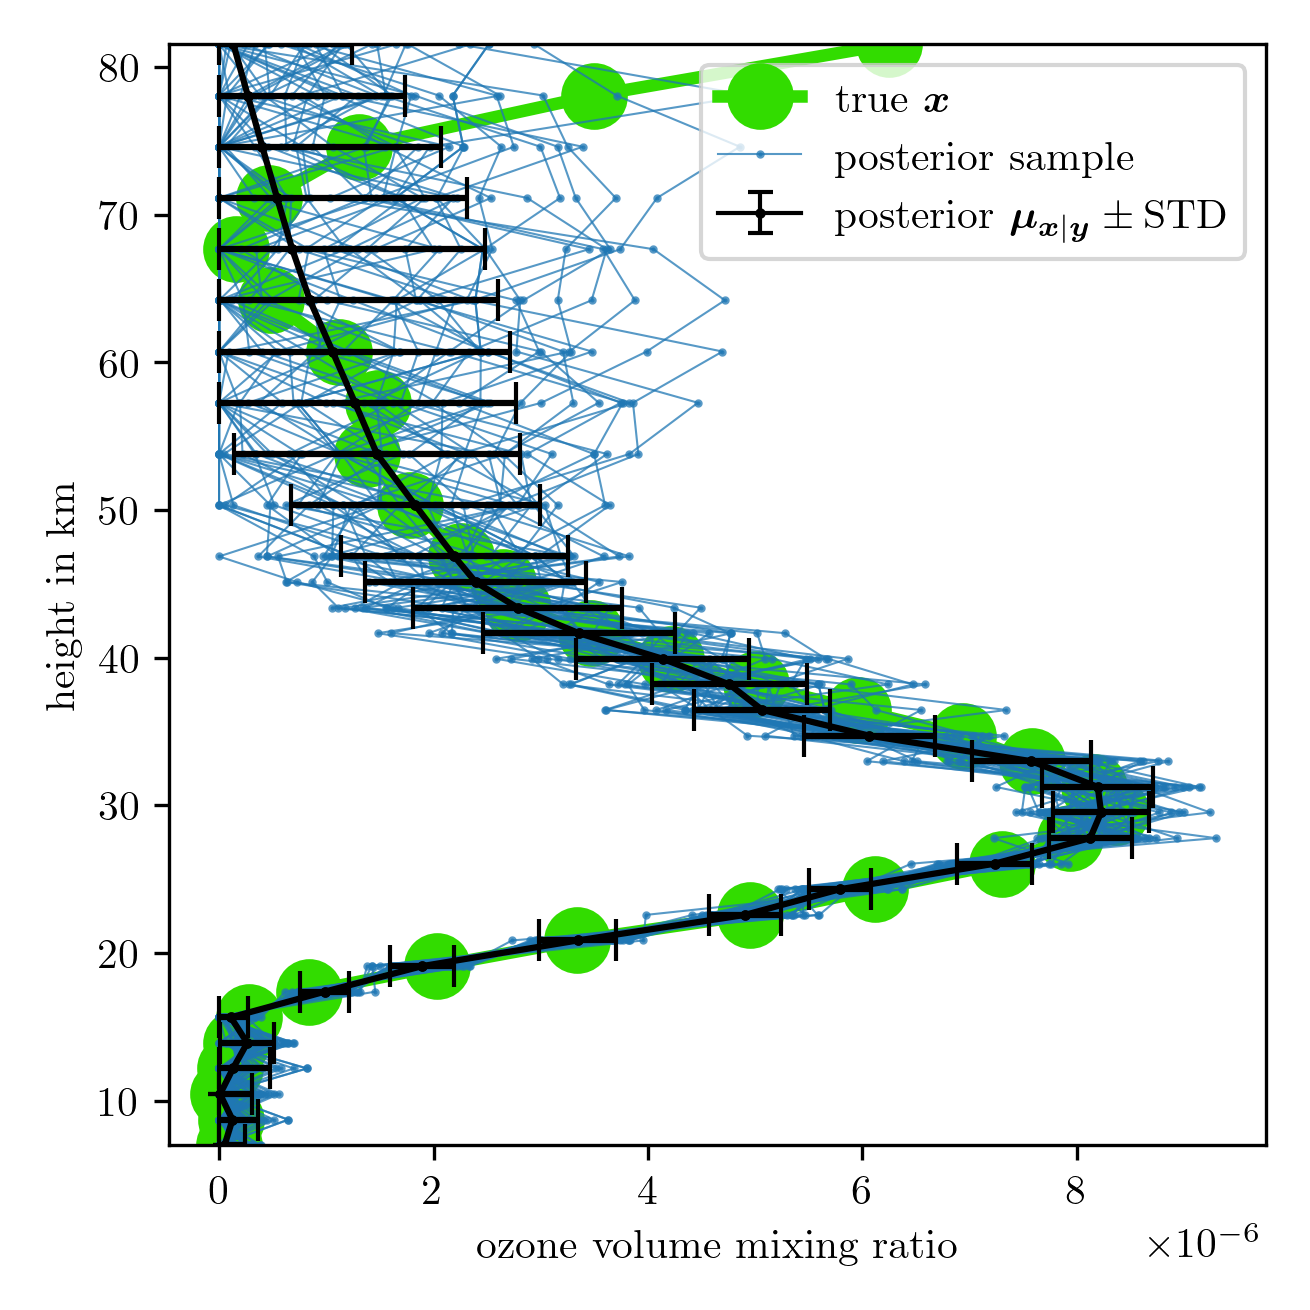
\includegraphics{FirstTestRes.png}
	\caption[Ozone samples of the conditional posterior.]{We draw samples from the conditional posterior distribution  $\pi(\bm{x}|\lambda,\gamma , \bm{y})$ after characterising the marginal posterior $\pi(\lambda,\gamma | \bm{y})$ through sampling or TT approximation using the linear forward map $\bm{A}_L$. Note that we reject samples with unphysical negative values and effectively treat the conditional posterior as a truncated multivariate normal distribution. We will use those samples to find the affine map $\bm{M}$, see section \ref{sec:affineMap}}
	\label{fig:O3Samp}
\end{figure}

%\subsubsection{Randomize then optimize -- RTO}
%For the RTO method we start by drawing an independent hyper-parameter sample $ ( \delta, \gamma) \sim \pi(\delta, \gamma | \bm{y})$ from the samples of the MwG.
%Then we generate two independent Gaussian random variables $\bm{v}_1 \sim \mathcal{N}(\bm{0},\gamma  \bm{A}^T_L \bm{A}_L)$ and $\bm{v}_2 \sim \mathcal{N}(\bm{0}, \delta \bm{L})$.
%Here  can use Cholesky factorisation of $\bm{L} =\bm{L}_C\bm{L}^T_C $ and the multiplication rule for normal distributions so that $\bm{v}_1 \sim \sqrt{\gamma} \bm{A}_L^T \mathcal{N}(0,\bm{I})$ and $\bm{v}_2 \sim \sqrt{\delta} \bm{L}_C \mathcal{N}(0,\bm{I})$.
%Then we solve
%\begin{align}
%	\label{eq:FirstRTO}
%	\left( \gamma \bm{A}_L^T  \bm{A}_L +\delta \bm{L} \right) \bm{x} = \gamma \bm{A}_L^T \bm{y} + \bm{v}_1 + \bm{v}_2 \, ,
%\end{align}
%using Cholesky back and forward substitution, for $\bm{x}$ and obtain one independent sample of $\pi(\bm{x}|\bm{y}, \bm{\theta})$.
%See Fig. \ref{fig:O3Samp}, where we plot $m = $ samples of the conditional posterior.
%
%The histogram in is binned as we intergate over it to 7 bins
\subsection{Asses approximated forward model}
Given $m$ samples $\bm{x}^{j} \sim \pi{\bm{x}|\bm{y}}$ for $j = 1, \dots,m$ from the full conditional, as plotted in\ref{fig:O3Samp}, we are able approximate the non-linear forward model
\begin{align}
	\bm{A}_{NL} \approx \bm{M A}_L = \bm{A} \, ,
\end{align}
with the affine map $\bm{M}$ and the linear forward model $\bm{A}_L$.
In doing so, we can generate two affine subspaces $\bm{W} = \{\bm{A}_L\bm{x}^1, \dots, \bm{A}_L\bm{x}^m \}$ and $\bm{V} = \{\bm{A}_{NL}\bm{x}^1, \dots, \bm{A}_{NL}\bm{x}^m \}$.
We use the Python function \texttt{numpy.linalg.solve} to solve $ \bm{M}\bm{W} = \bm{V}$ for each row of $ \bm{M}$, see Sec. \ref{sec:affine} for more details.



We asses the affine map by calculating the relative error\textcolor{red}{ $|| \bm{M}\bm{W} - \bm{V}  || / || \bm{M}\bm{W} ||$ } between the mapped noise free data and the noise free data of non-linear forward model for all of the $m$ ozone samples, which approximnately $0.1$\%
We display the approximation for one $\bm{x}$ sample in Fig. \ref{fig:MapAsses}.
Consequently, from here onwards, we use the approximated forward map $\bm{A} = \bm{M A}_L $.
\begin{figure}[ht!]
	\centering
	%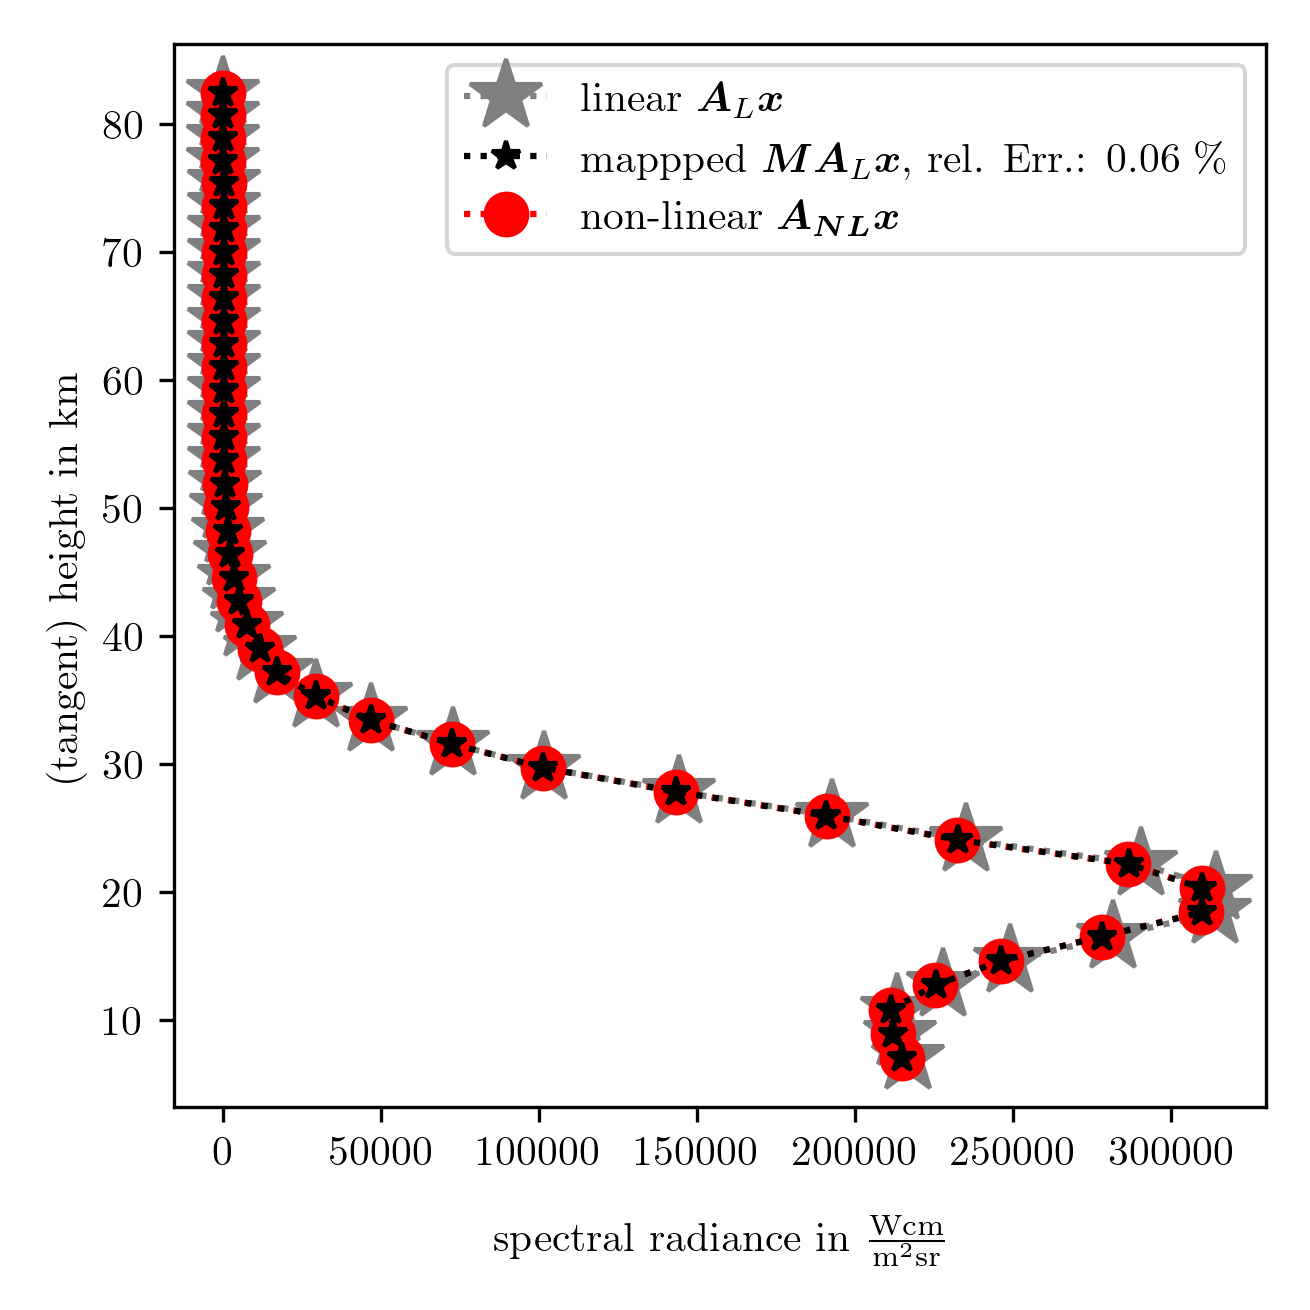
\includegraphics{SampMapAssesment.png}
	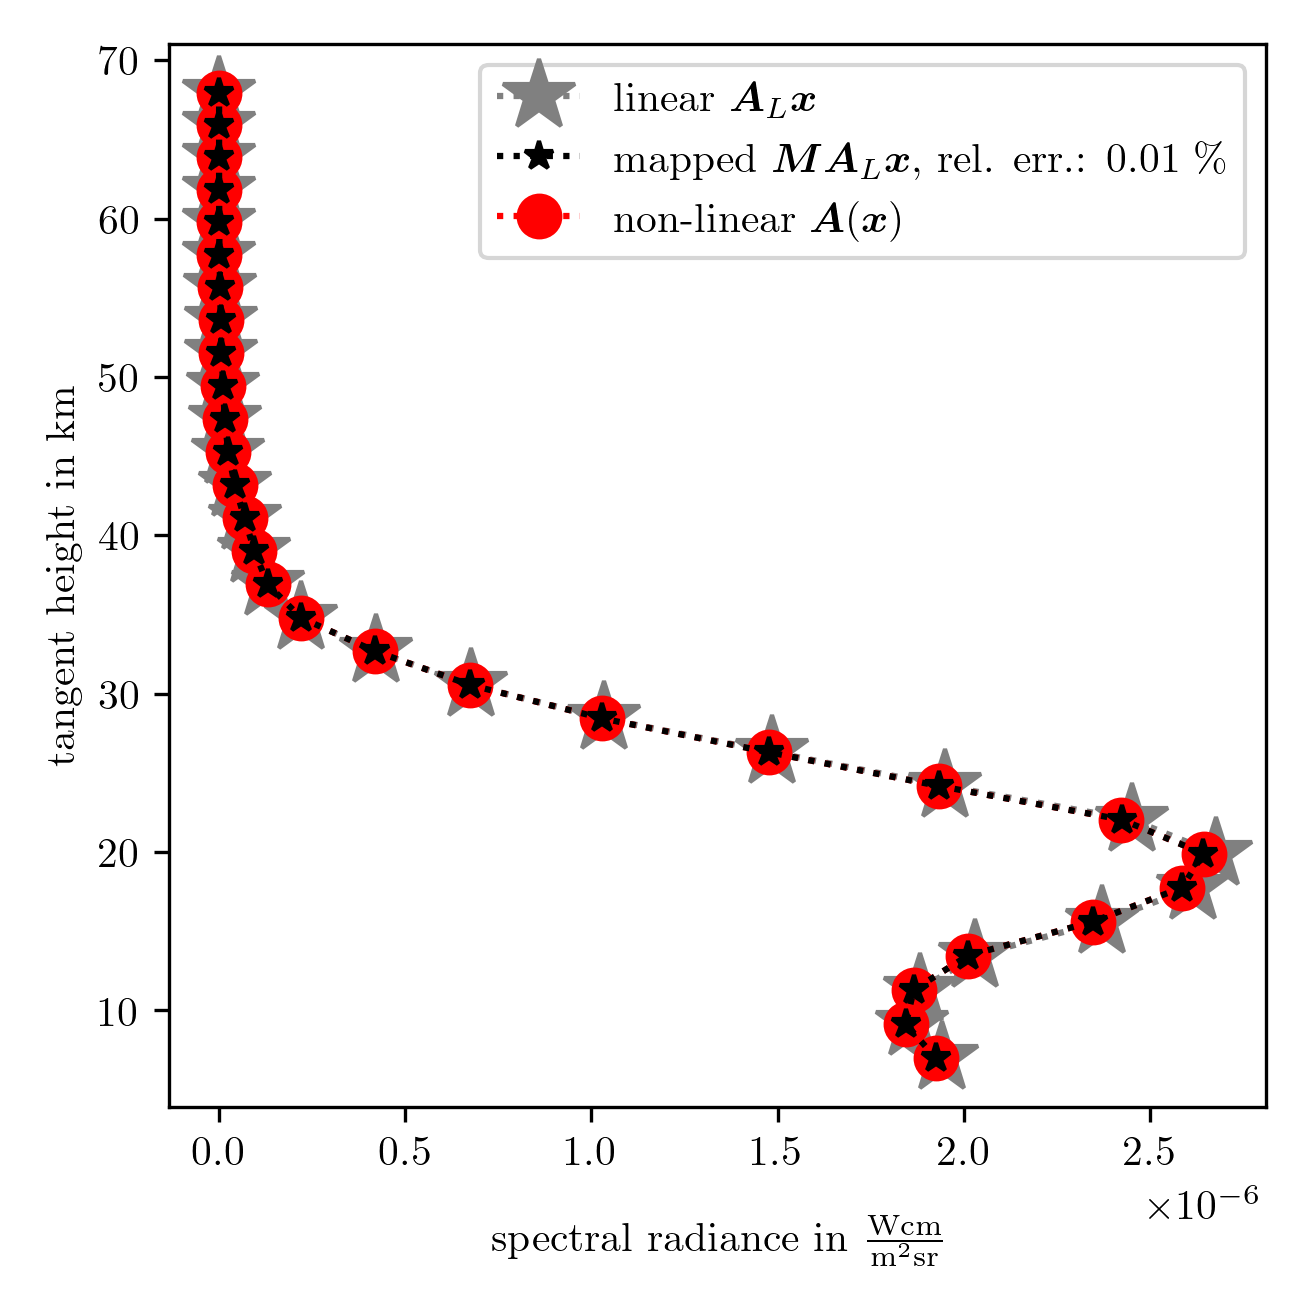
\includegraphics{SampMapAssesmentTT.png}
	\caption[Assessment of affine map.]{We asses how good we can map the linear forward model onto the non-linear forward model using the previous calculated affine map. The gray stars represent noise free linear data, where as the red circles present noise free non-linear data. Then we map the linear noise free data onto the non-linear noise free data and give the relative error in between the mapped noise free data and the non-linear data.}
	\label{fig:MapAsses}
\end{figure}

%$|| \bm{M}\bm{A}_L \bm{x} - \bm{A}_{NL} \bm{x} || / || \bm{M}\bm{A}_L \bm{x} ||$

\section{Solution by regularisation}
\label{sec:reg}
Since we like to compare the MTC method to regularisation methods, we calculate a solution by Tikhonov regularisation, as this is most similar to our chosen linear-Gaussian Bayesian framework.
The Tikhonov regularised solution is defined as~\cite{hansen2010discrete} 
\begin{align}
	\bm{x}_{\lambda} =\underset{ \bm{x}}{\arg \min}\,  \lVert \bm{A}\bm{x} - \bm{y} \rVert_2^2 + \lambda \bm{x}^T \bm{L} \bm{x} \, ,
	\label{eq:XLam}
\end{align}
with the regularisation parameter $\lambda = \delta / \gamma$.
The regularised solution is typically calculated by solving the normal equations, see Sec. \ref{sec:regularise},
\begin{align}
	\bm{x}_{\lambda} = (\bm{A}^T\bm{A} + \lambda \bm{L} )^{-1} \bm{A}^T \bm{y} \label{eq:xLam} \, .
\end{align}
To find the best regularised solution, we use the L-curve method~\cite{hansen1993use}.
Within this method we compute $\bm{x}_\lambda$, for 200 different $\lambda$ values in between $1$ to $10^7$ and plot the solution semi norm $\sqrt{\bm{x}_\lambda^T\mathbf{L} \bm{x}_\lambda}$ against the data misfit norm $\lVert \bm{A}\bm{x}_\lambda - \bm{x} \rVert$, see Figure \ref{fig:LCurve}. 
The best regularised solution corresponding to the corner of the L-curve is located at the point of maximum curvature, see triangle in Fig. \ref{fig:LCurve}, which we find with the kneedle algorithm~\cite{satopaa2011kneedle} using the python function \texttt{kneed.KneeLocator} in less $0.1$s.

\begin{figure}[ht!]
	\centering
	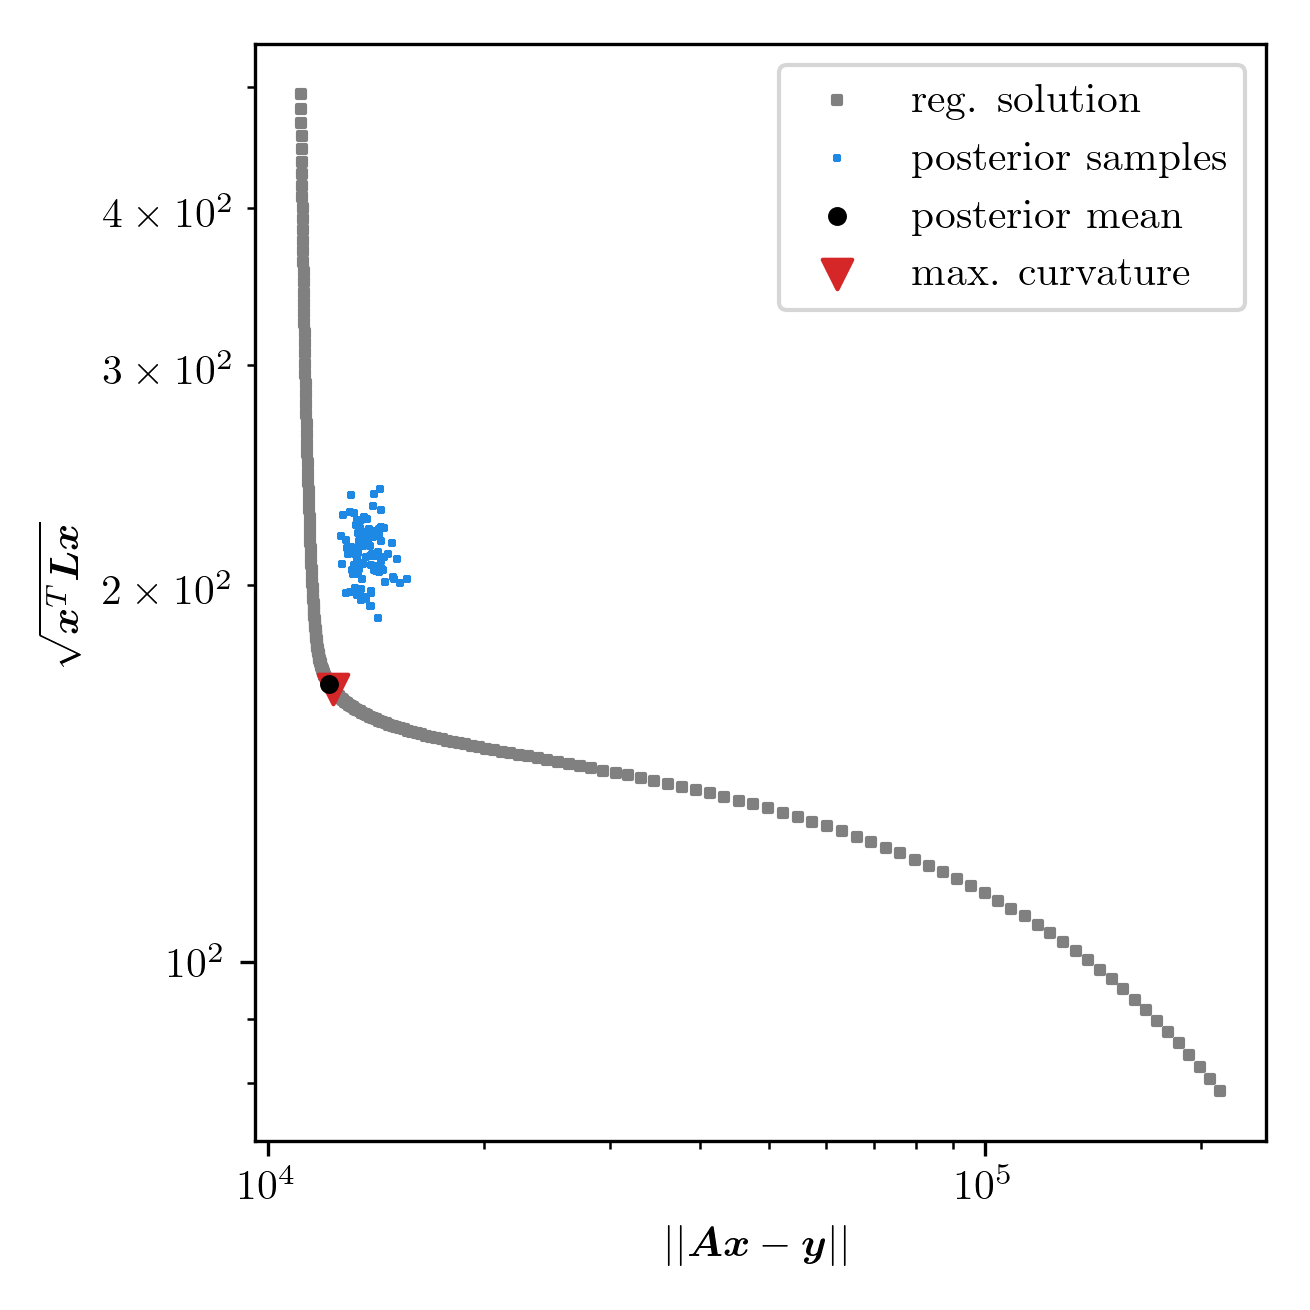
\includegraphics{LCurvePhD.png}
	\caption[Plot of the L-curve to find the regularised solution.]{We calculate regularised solution as in Eq. \ref{eq:} and plot the regularised semi norm $\sqrt{\bm{x}^T\bm{Lx}}$ against the data misfit norm $||\bm{Ax} -\bm{y} ||$ to find the regularised solution at the point of maximum curvature of the so-called L-Curve. Additionally we calculate the data misfit norm and the regularised norm for the ozone posterior and for samples of the conditional posterior distribution. \textcolor{red}{make box around Kneedle reagion}}
	\label{fig:LCurve}
\end{figure}


\section{Characterise the posterior distribution of ozone with approximated forward model}
With the affine approximation
\begin{align}
	\bm{A} =  \bm{M A}_L \, 
\end{align}
of the non-linear forward map, we use the same setup as in Sec. \ref{sec:firstMarg} and \ref{subsec:firstCond} to evaluate the marginal posterior and the conditional posterior.

\subsection{Hyper-parameters samples from and Tensor-train approximation of the marginal posterior distribution}
The marginal posterior is defined as in Eq. \ref{eq:marg} but with $ \bm{A} =  \bm{M A}_L$.
We run the MWG algorithm for $N = 20000$ plus $N_{\text{burn-in}} = 100$ and plot the samples in Fig. \ref{fig:MargPostHistTT} as well as the marginal approximations provided by the TT decomposition, where we use the same setup as in Sec. \ref{sec:firstMargTT}.

\begin{figure}[ht!]
	\centering
	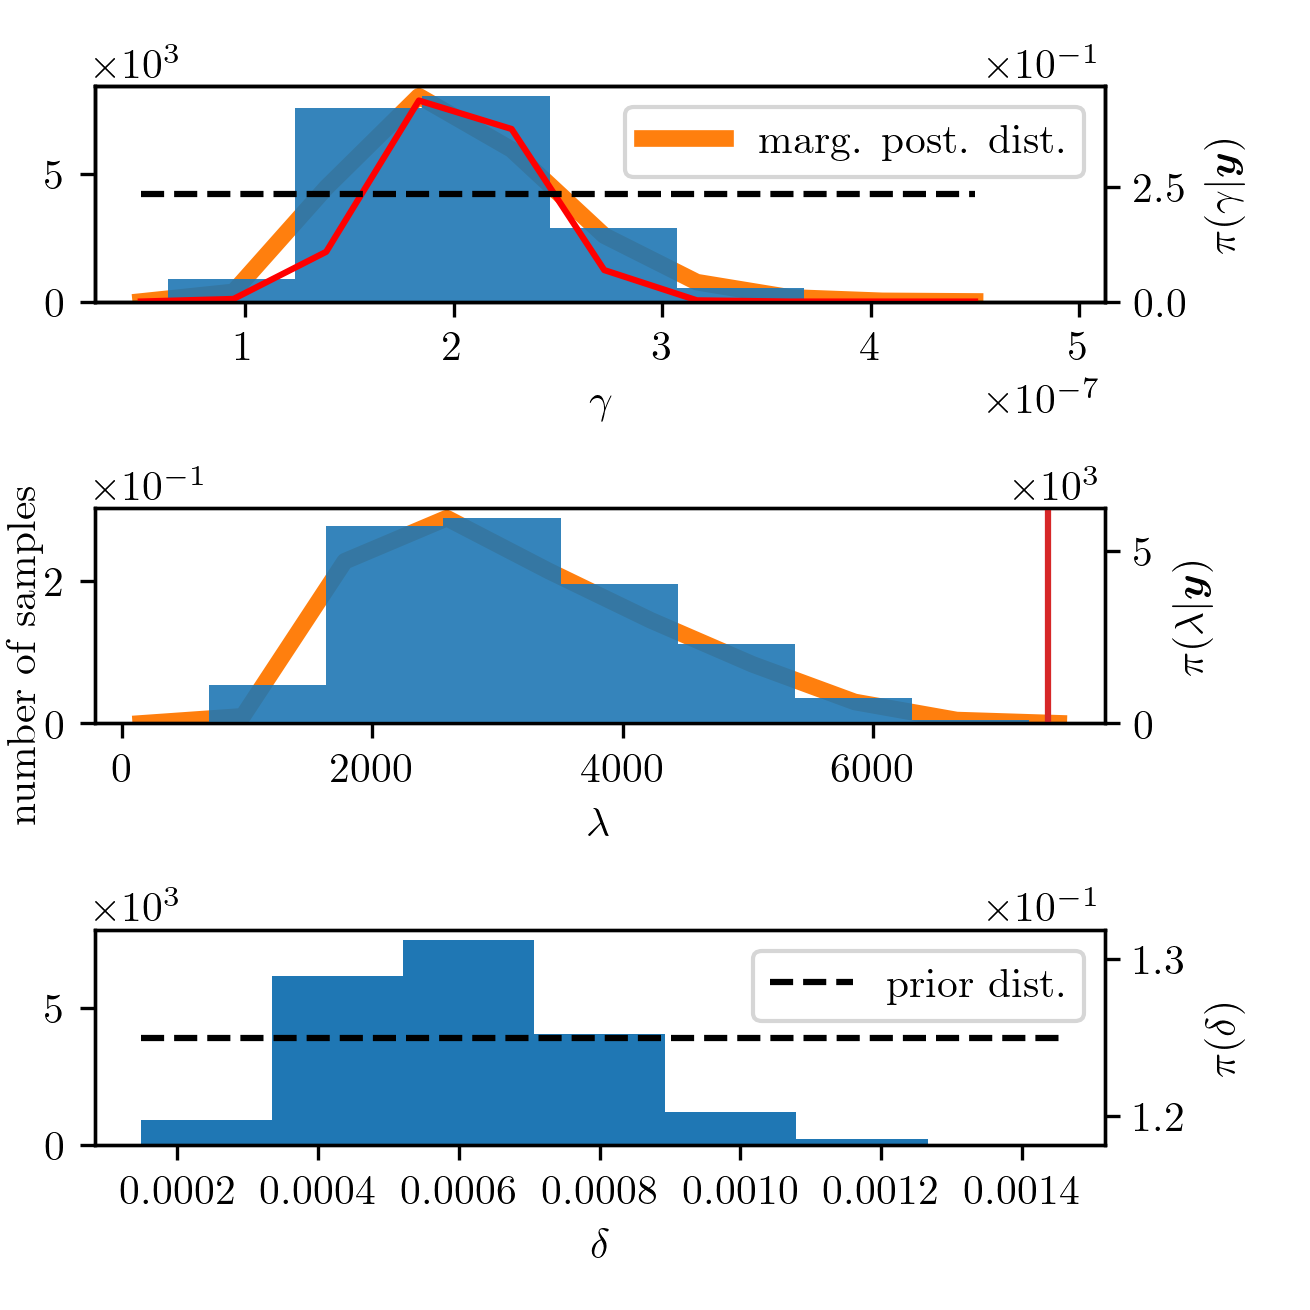
\includegraphics{secSIRTMargMargO3Res.png}
	\caption[Marginal posterior histograms and TT approximation as well as hyper-prior distribution.]{We plot the TT approximation of marginal posterior in orange and the samples as a histogram as well as the prior distribution with a dotted line. Note that we sample $\lambda$ and $\gamma$ using the Metropolis-within-Gibbs sampler and can calculate $\delta$ for every sample of the marginal posterior, we can not do this for the TT approximation. The regularised parameter corresponding to the regularised solution is marked thought the red vertical line at $\lambda_{\text{reg}} =$.}
	\label{fig:MargPostHistTT}
\end{figure}

\subsection{Full conditional posterior variance and mean}
Next, we characterise the conditional posterior $\pi(\bm{x}|\gamma, \delta, \bm{y})$ as in Eq. \ref{eq:CondPost}. 
Again, we calculate the full conditional mean \ref{eq:MeanInt} and full conditional covariance matrix \ref{eq:CovInt} as weighted expectation over a 25-point grid provided by either the marginal TT approximations or the histogram of samples.
We plot the conditional mean and variance in Fig. \ref{fig:O3SolplsReg} and the regularised solution and one sample from the posterior.
\begin{figure}[ht!]
	\centering
	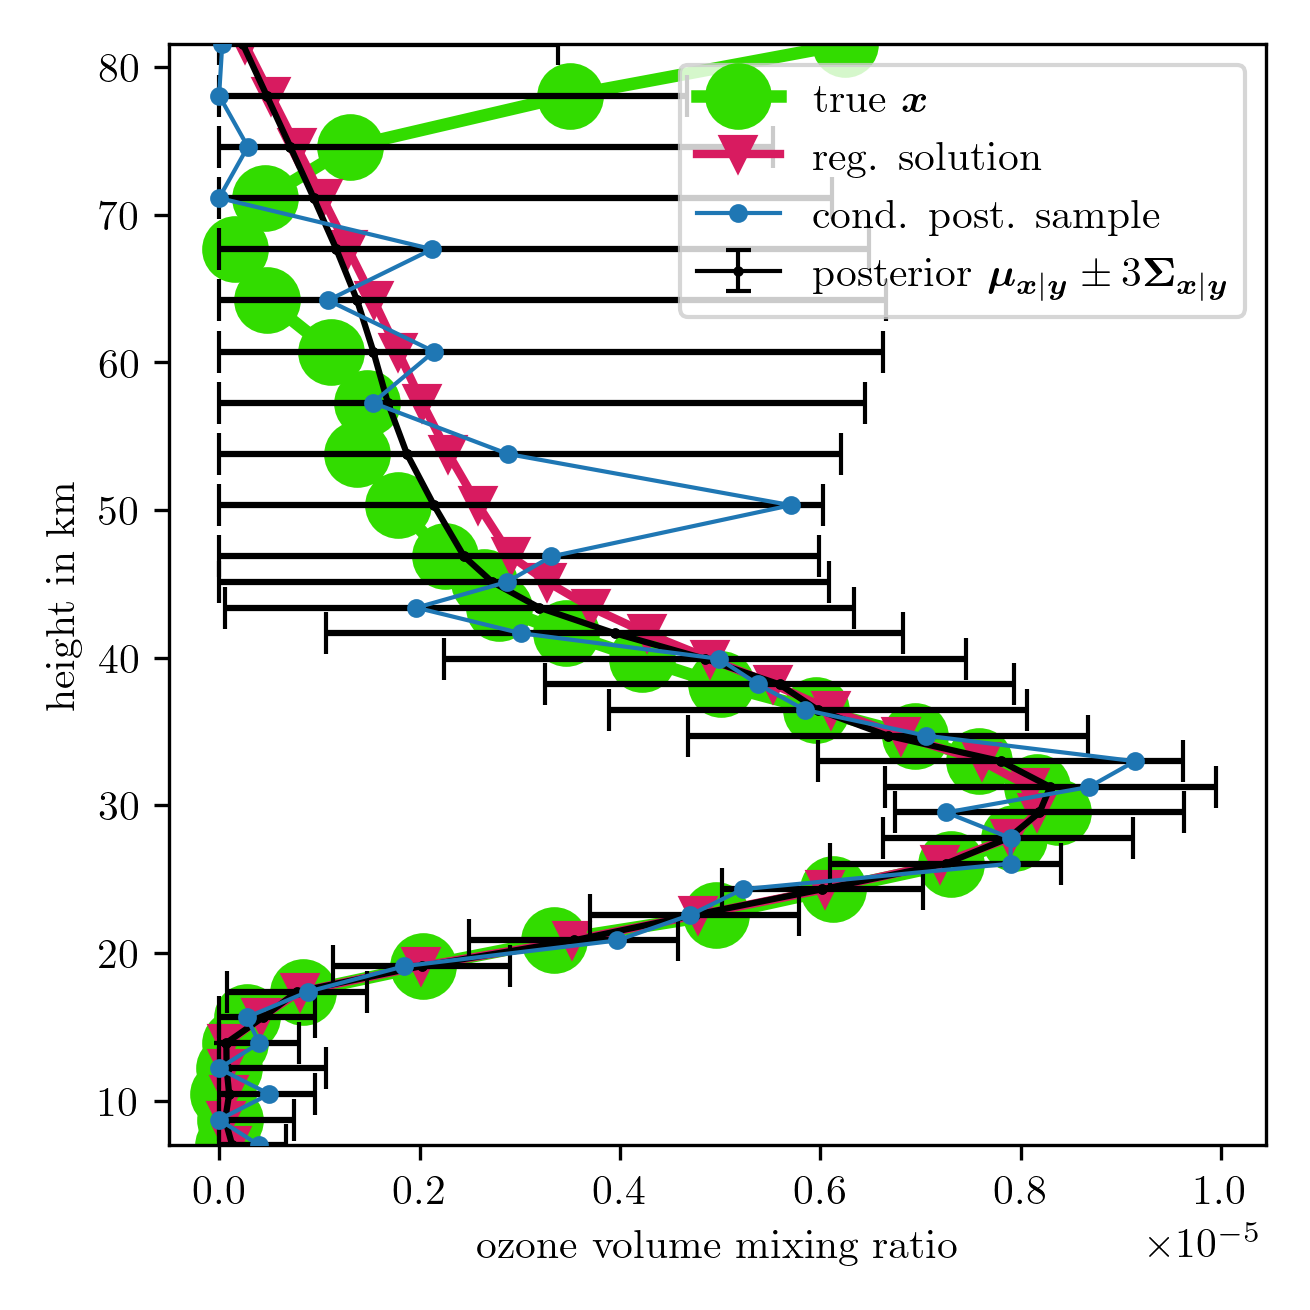
\includegraphics{SecRecResinclRegandSampl.png}
	%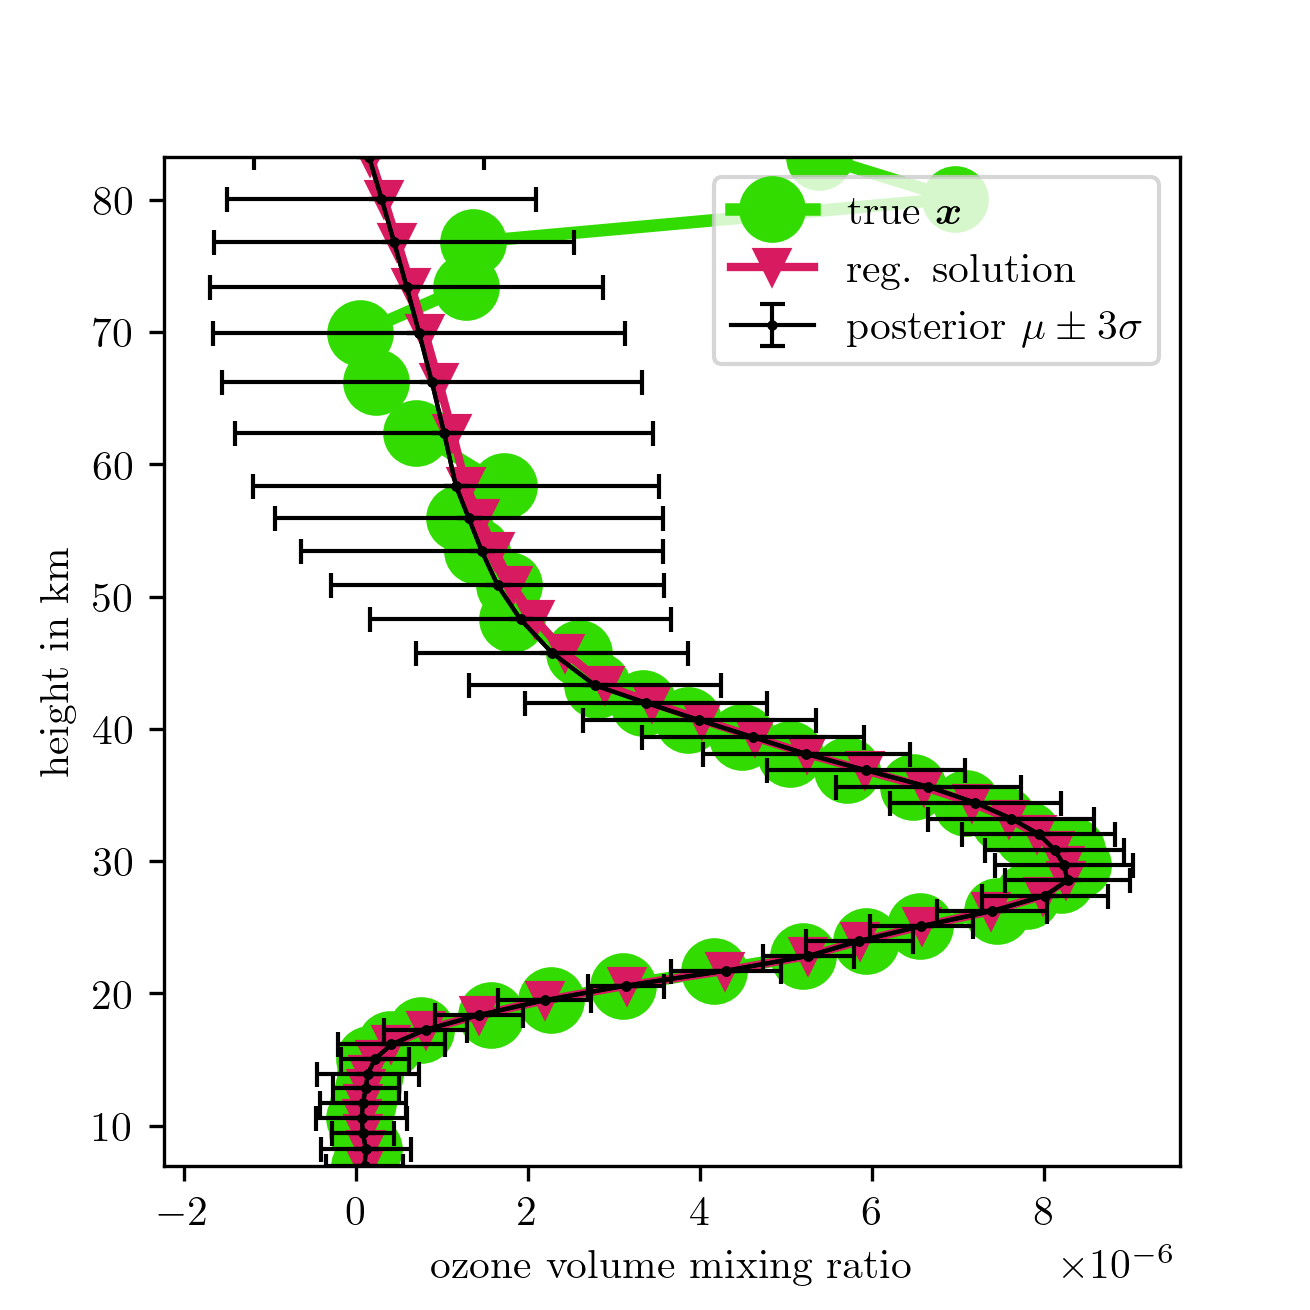
\includegraphics{SecRecResinclReg.png}
	\caption[Ozone posterior mean and variance and the regularised solution compared to the ground truth.]{We plot the conditional posterior mean and variance in black and the regularised solution on top of the ground truth ozone profile in green. We use the updated forward map $\bm{M}\bm{A}_L$}
	\label{fig:O3SolplsReg}
\end{figure}

\begin{figure}[ht!]
	\centering
	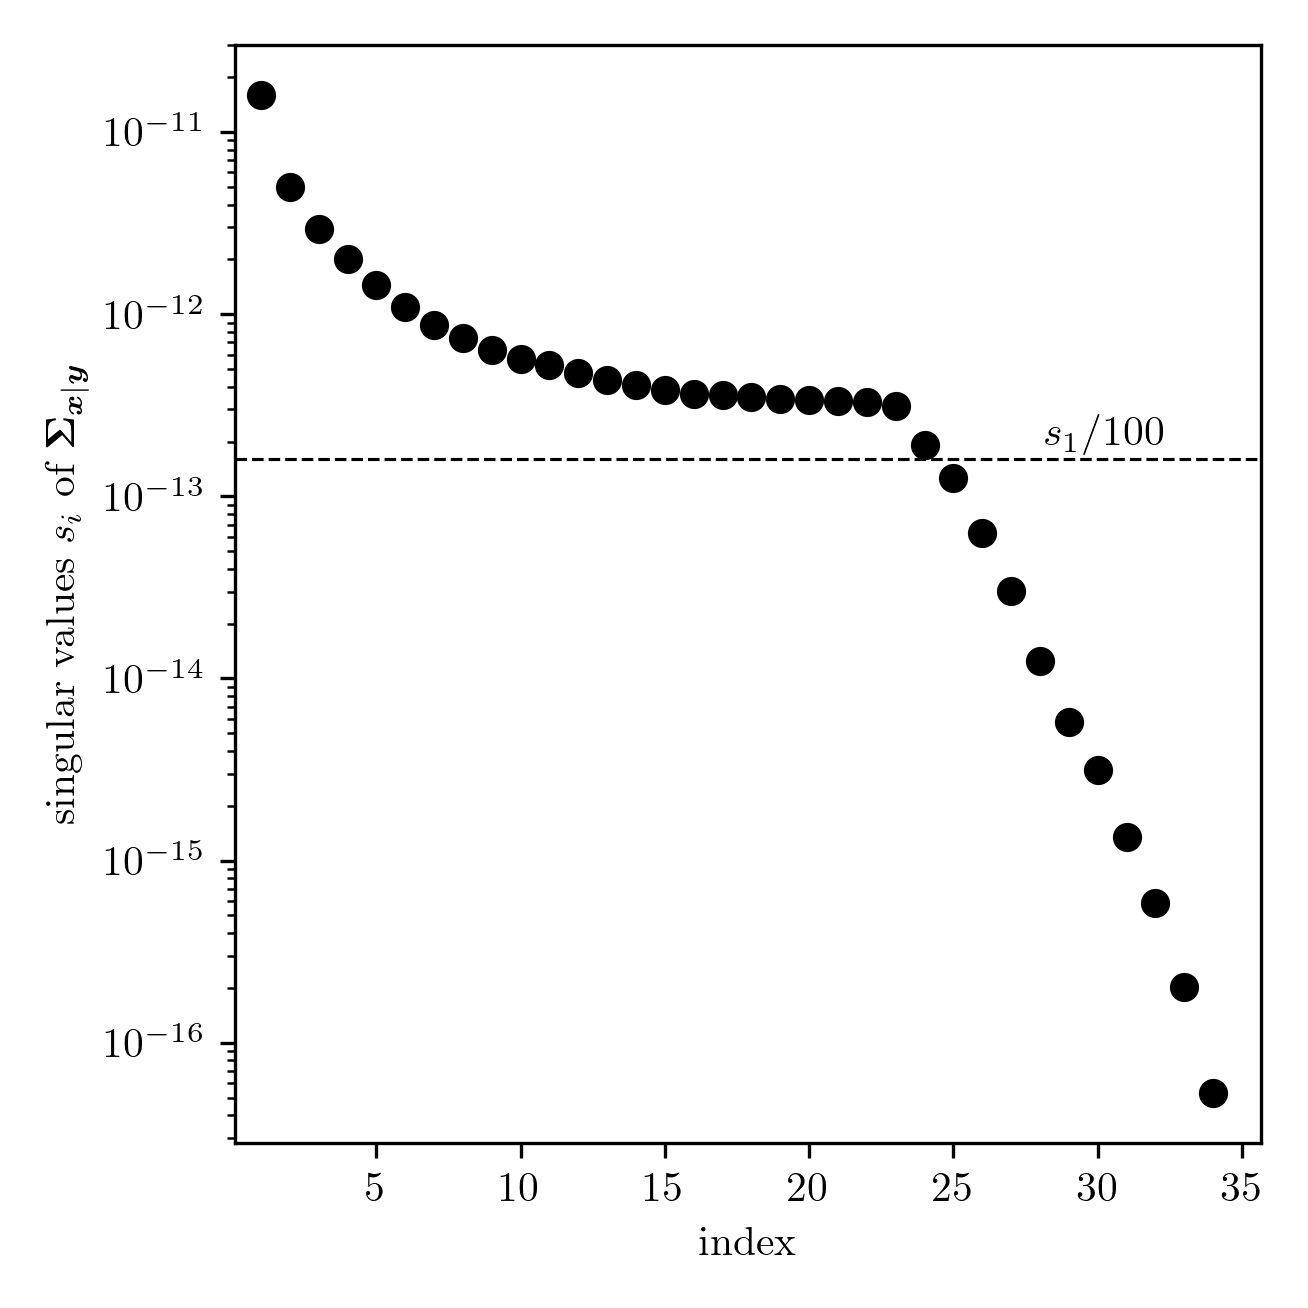
\includegraphics{CovSing.png}
	\caption[]{}
	\label{fig:}
\end{figure}

\clearpage

\section{Posterior distribution for pressure and temperature with approximated forward model}
\label{sec:postPT}

The aim now is to characterise the posterior
\begin{align}
	\begin{split}
		\pi(p_0,b,T_0,\bm{h_T},\bm{a_T} | \bm{y}, \gamma, \bm{x}) \propto  \exp\Bigl\{ & -\frac{\gamma}{2} \left\Vert \bm{y}- \bm{A} \frac{\bm{p}}{\bm{T}}  \right\Vert^2 \\ &+ \ln{\pi(p_0,b,T_0,\bm{h_T},\bm{a_T}) \Bigr\}  }
	\end{split} \, ,
	\label{eq:postPT}
\end{align}
conditioned on the ozone sample in Fig. \ref{fig:O3SolplsReg} and a $\gamma$ sample from the marginal posterior, and using the approximated forward model $\bm{A} = \bm{M}\bm{A}_L$.
We will approximate this posterior with a TT and validate this approximation with samples from the posterior using the \texttt{t-walk} \cite{christen2010general} implementation in Python \cite{christentwalkaccess}.
“Conditioning
on estimates gives poor predictive densities”.
\cite{tan2016LecNot}

Again, we define a grid with 25 grid points in each dimension, which also acts as the sampling space.
Since we approximate a 16-dimensional function, we have to carefully choose a grid, as we do not want to approximate regions with low probability, and we like to keep the number of grid points low, as this increases computation time.
We find the grid, see Tab. \ref{tab:priors}, iteratively by running the t-walk and then computing marginal distributions.
Note that we bound the sampling space of the t-walk by the TT-grid.
We run the  \texttt{tt.cross.rectcross.rect\_cross.cross} function from the \texttt{ttpy} python package \cite{} with constant rank $r = 16$, equal to the dimension of the posterior.
Next, we introduce a constant $c$ in the posterior, which acts as a normalisation constant and is needed when approximating the square root of the posterior for pressure and temperature with a tensor-train (TT) to avoid underflow.
Then the posterior becomes:
\begin{align}
	\begin{split}
		\pi(p_0,b,T_0,\bm{h_T},\bm{a_T} | \bm{y}, \gamma, \bm{x}) \propto  \exp\Bigl\{ & -\frac{\gamma}{2} \left\Vert \bm{y}- \bm{A} \frac{\bm{p}}{\bm{T}}  \right\Vert^2 \\ &+ \ln{\pi(p_0,b,T_0,\bm{h_T},\bm{a_T}) + c \Bigr\}  }
	\end{split} \, .
	\label{eq:TTpostPT}
\end{align}
To find the constant $c$, we evaluate the logarithm of the posterior on 5000 random points and calculate the maximum $c_{\text{max}} < 0$ of those 5000 points.
Then we set the constant to a value which pushes the posterior close to the upper numerical limit of our machine, which is approximately $e ^{700}$.
Since we approximate the square root, we conservatively set the constant to $c = -c_{\text{diff}} + 325$.
It takes roughly $3$ to $4$min for 15 sweeps by the \texttt{cross} to find the optimal tensors.
Then we can compute the marginal as in Sec. \ref{sec:tensortrain}, where we set $\xi = 1 / \uplambda (\mathcal{X})$.

For comparison, we run the t-walk on the posterior as defined in Eq. \ref{eq:postPT} for $5 \times 10^6$ steps plus a burn-in period of $10000$, which takes around $7$ mins on the same laptop.
We plot the resulting histograms in Fig. \ref{fig:PostHistTT0} to \ref{fig:PostHistTT4}; additionally, we plot the trace of the samples in Fig. \ref{fig:TraceTwalk}.
The integrated autocorrelation times (IACT) for the hyper-parameters range from $0$ to $1000$ and are summarised in Tab. \ref{tab:priors}.
%\begin{figure}[thb!]
%	\centering
%	\begin{tikzpicture}
%		
%		\node[align=center] at (-1,4) (A)    {$\bm{M A}_L$};
%		\node[roundnode2] at (-1,2.5) (u)    {$\bm{u}$};
%		\node[rectnode] at (-1,1) (y)    {$\bm{y}$};
%		
%		\node[roundnode2] at (3,6.5) (t)     {$\bm{T}$};
%		\node[roundnode2] at (-1,6.5) (p)     {$\bm{p}$};
%		\node[roundnode2] at (1,5) (pt)     {$\bm{p}/\bm{T}$};
%		\node[roundnode2] at (0,8) (b1)    {$b$};
%		%\node[roundnode2] at (1,8) (b2)    {$b_2$};
%		\node[roundnode2] at (-2,8) (h1)    {$h_0$};
%		\node[roundnode2] at (-1,8) (p0)    {$p_0$};
%		\node[roundnode2] at (2.25,8) (ht)    {$\bm{h}$};
%		\node[roundnode2] at (3.25,8) (ct)    {$T_0$};
%		\node[roundnode2] at (4.25,8) (at)    {$\bm{a}$};
%		
%		%Lines
%		\draw[->, very thick] (u.south) -- (y.north);
%		\draw[->, mydotted, very thick] (A.south) -- (u.north);
%		
%		\draw[->, mydotted, very thick] (p.south east) -- (pt.north west);
%		\draw[->, mydotted, very thick] (t.south west) -- (pt.north east);
%		\draw[->, mydotted, very thick] (pt.south west) -- (A.east);
%		\draw[->, mydotted, very thick] (h1.south) -- (p.north west);
%		\draw[->, mydotted, very thick] (p0.south) -- (p.north);
%		\draw[->, mydotted, very thick] (b1.south) -- (p.north east); 
%		%\draw[->, very thick] (b2.south) -- (p.east); 
%		
%		\draw[->, mydotted, very thick] (ht.south) -- (t.north west);
%		\draw[->, mydotted, very thick] (ct.south) -- (t.north);
%		\draw[->, mydotted, very thick] (at.south) -- (t.north east);
%		
%		\node[align =center] at (-5,8) (T1) {posterior \\ over hyper-parameters \\ $\pi(h_0, p_0, b, \bm{h}, T_0, \bm{a}| \bm{y})$};
%		
%		\node[fit=(h1)(at),draw,dotted,black, rounded corners] {};
%	\end{tikzpicture} 
%	\caption[Directed acyclic Graph for pressure and temperature.]{Conditioned on an ozone profile the posterior of the hyper-parameters describing pressure and temperature is given as in Eq. \ref{eq:}. Since pressure and temperature go into the forward model as $\bm{p}/\bm{T}$ they are highly correlated but the pressure is the dominant parameter, see Fig. 
%		\ref{fig:PriorPressOverTemp} and \ref{fig:SeaLevelHist}. Note that here we use the updated forward model $\bm{M} \bm{A}_L$ and conditioned on a $\gamma$ sample from the previously evaluated marginal posterior see Fig. \ref{fig:MargPostHistTT}. }
%	\label{fig:DAGPT}
%\end{figure}
\begin{figure}[ht!]
	\centering
	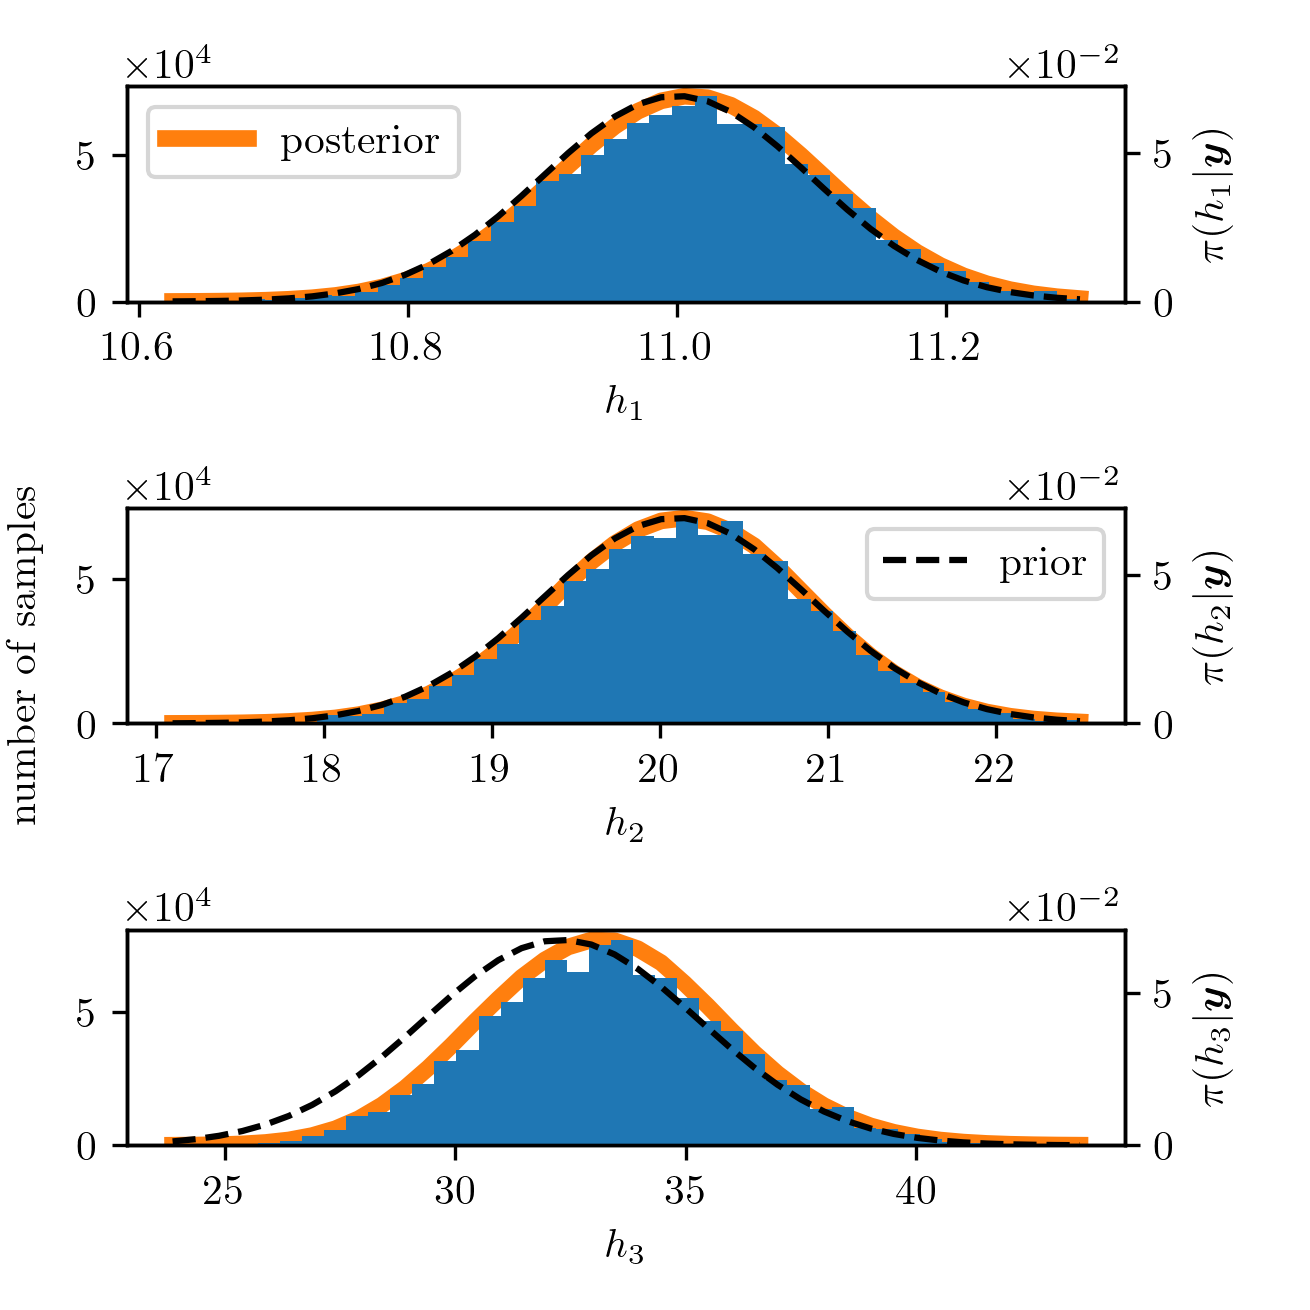
\includegraphics{PHdPTPost0.png}
	\caption[Histograms and TT approximation of posterior distribution as well as hyper-prior distribution.]{We plot the TT approximation of marginal posterior in orange and the samples as a histogram as well as the prior distribution with a dotted line.}
	\label{fig:PostHistTT0}
\end{figure}
\begin{figure}[ht!]
	\centering
	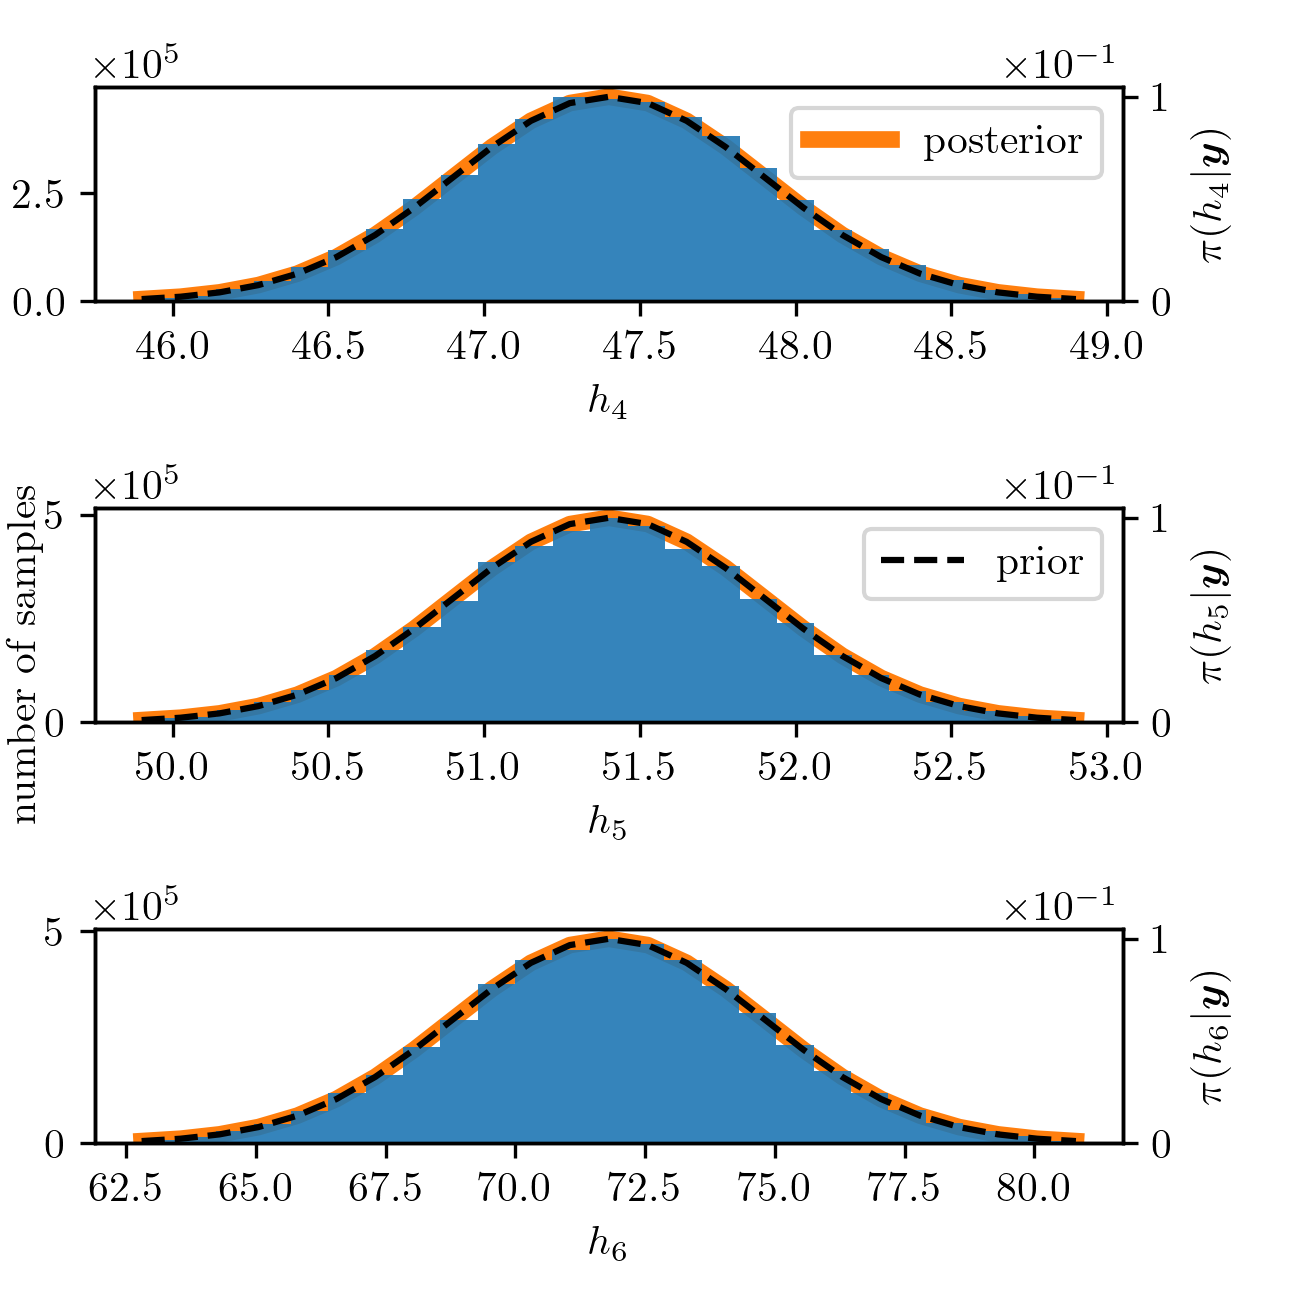
\includegraphics{PHdPTPost1.png}
	\caption[Histograms and TT approximation of posterior distribution as well as hyper-prior distribution.]{We plot the TT approximation of marginal posterior in orange and the samples as a histogram as well as the prior distribution with a dotted line.}
	\label{fig:PostHistTT1}
\end{figure}
\begin{figure}[ht!]
	\centering
	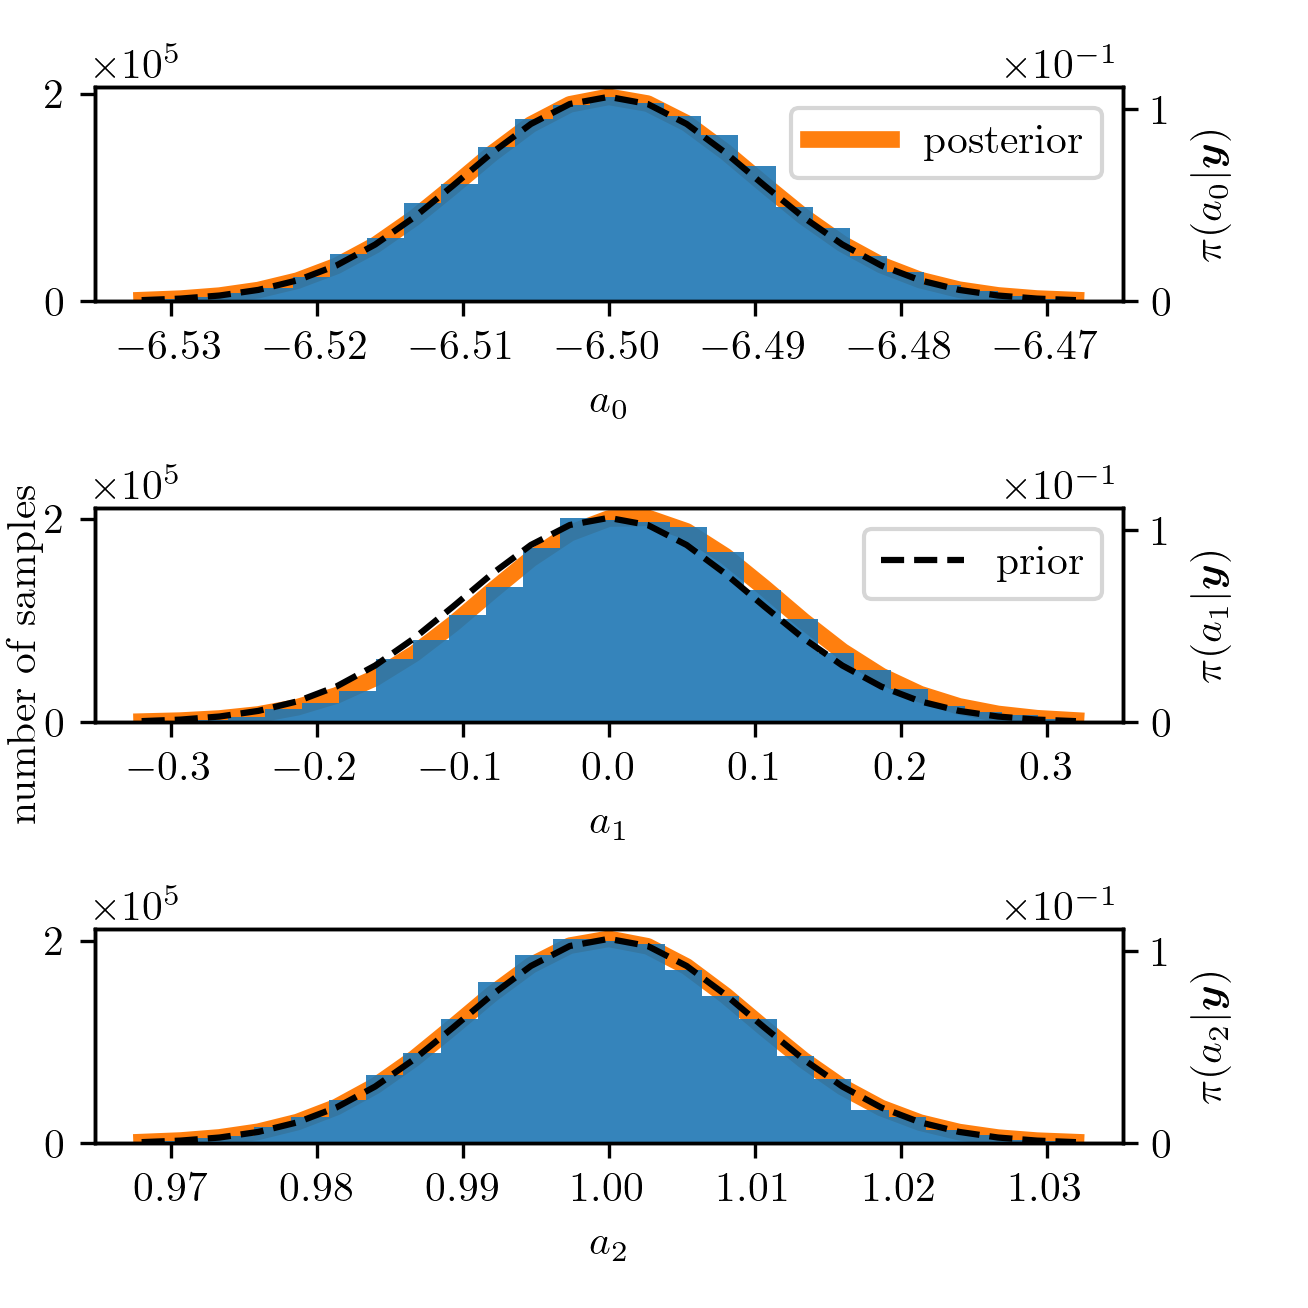
\includegraphics{PHdPTPost2.png}
	\caption[Histograms and TT approximation of posterior distribution as well as hyper-prior distribution.]{We plot the TT approximation of marginal posterior in orange and the samples as a histogram as well as the prior distribution with a dotted line.}
	\label{fig:PostHistTT2}
\end{figure}
\begin{figure}[ht!]
	\centering
	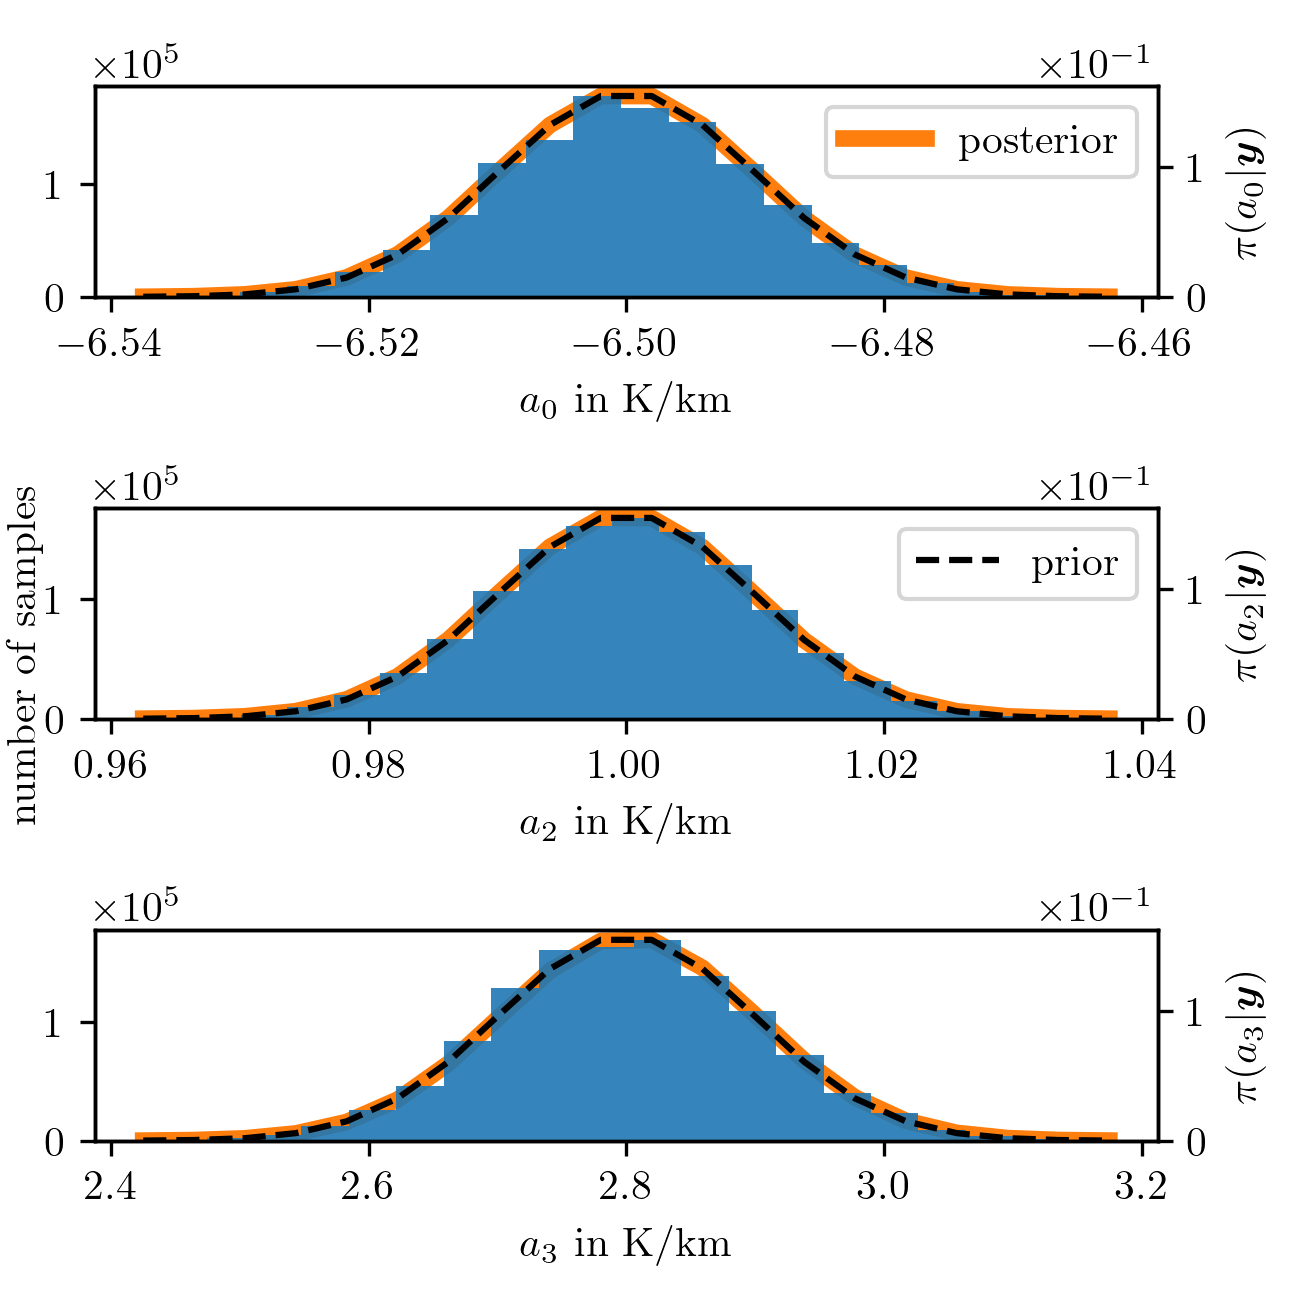
\includegraphics{PHdPTPost3.png}
	\caption[Histograms and TT approximation of posterior distribution as well as hyper-prior distribution.]{We plot the TT approximation of marginal posterior in orange and the samples as a histogram as well as the prior distribution with a dotted line.}
	\label{fig:PostHistTT3}
\end{figure}
\begin{figure}[ht!]
	\centering
	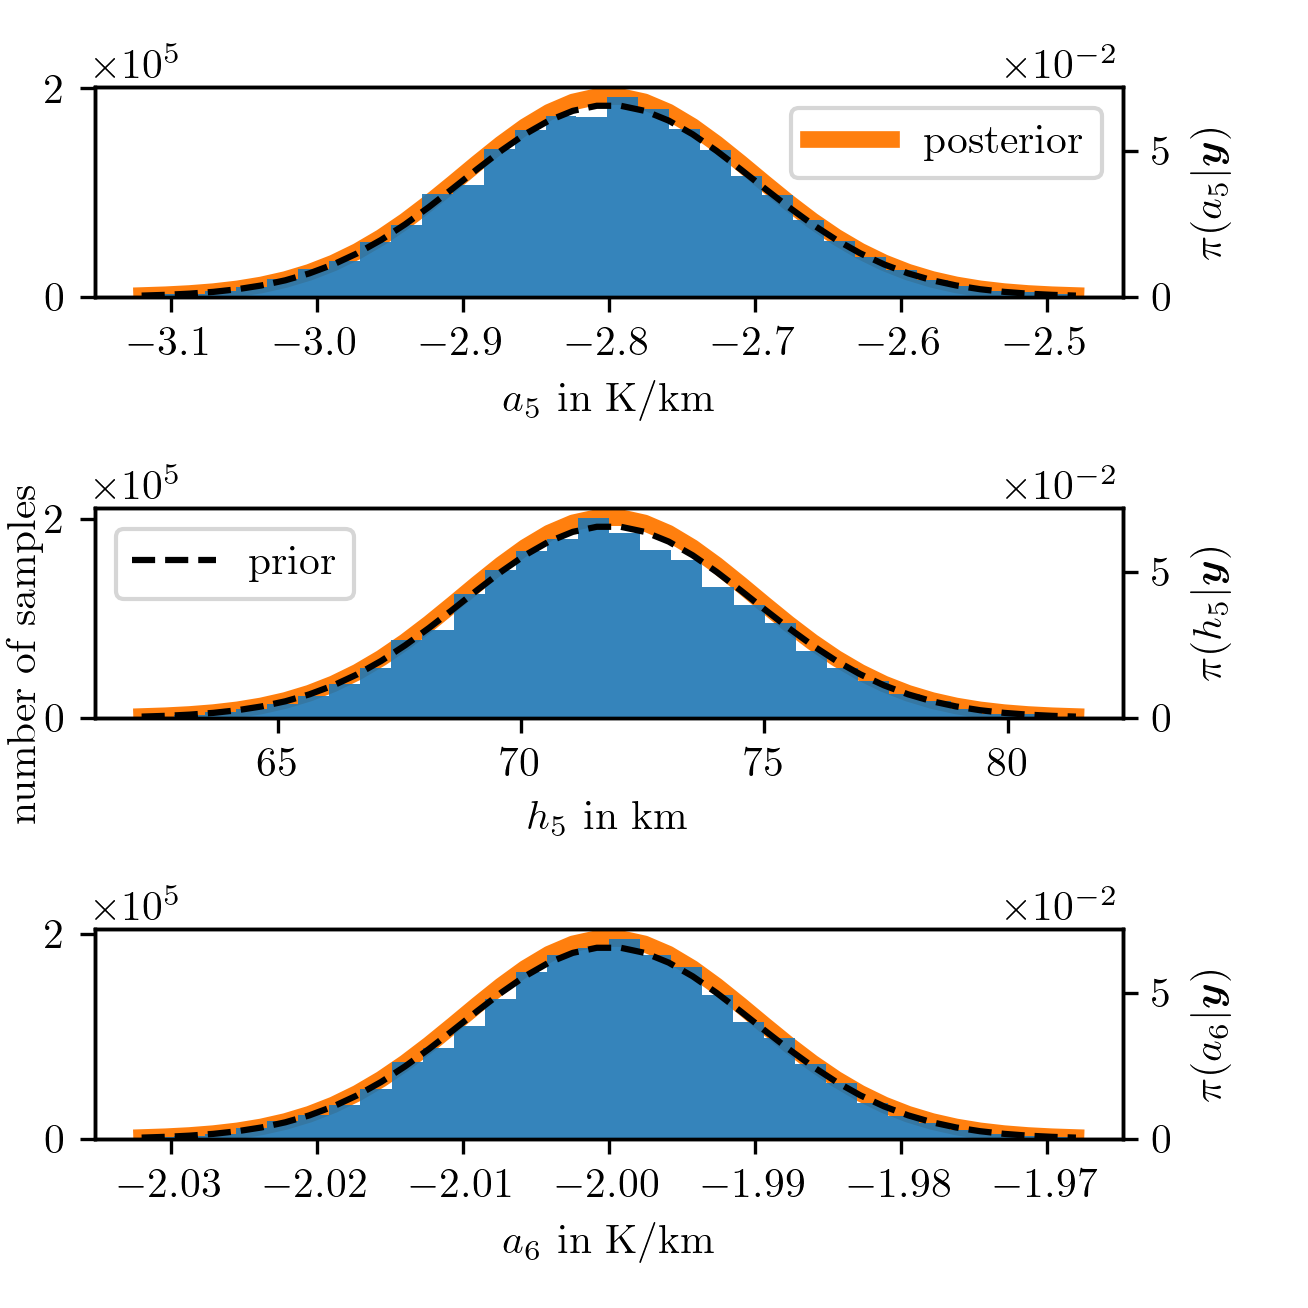
\includegraphics{PHdPTPost4.png}
	\caption[Histograms and TT approximation of posterior distribution as well as hyper-prior distribution.]{We plot the TT approximation of marginal posterior in orange and the samples as a histogram as well as the prior distribution with a dotted line.}
	\label{fig:PostHistTT4}
\end{figure}
\clearpage
To obtain temperature and pressure profiles, we can either take samples from the output of the t-walk or generate random values between 0 and 1 and compare them to the cumulative distribution functions.
We plot the posterior temperature and pressure profiles in Fig. \ref{fig:TempPost} and Fig. \ref{fig:PressPost}.
\begin{figure}[ht!]
	\centering
	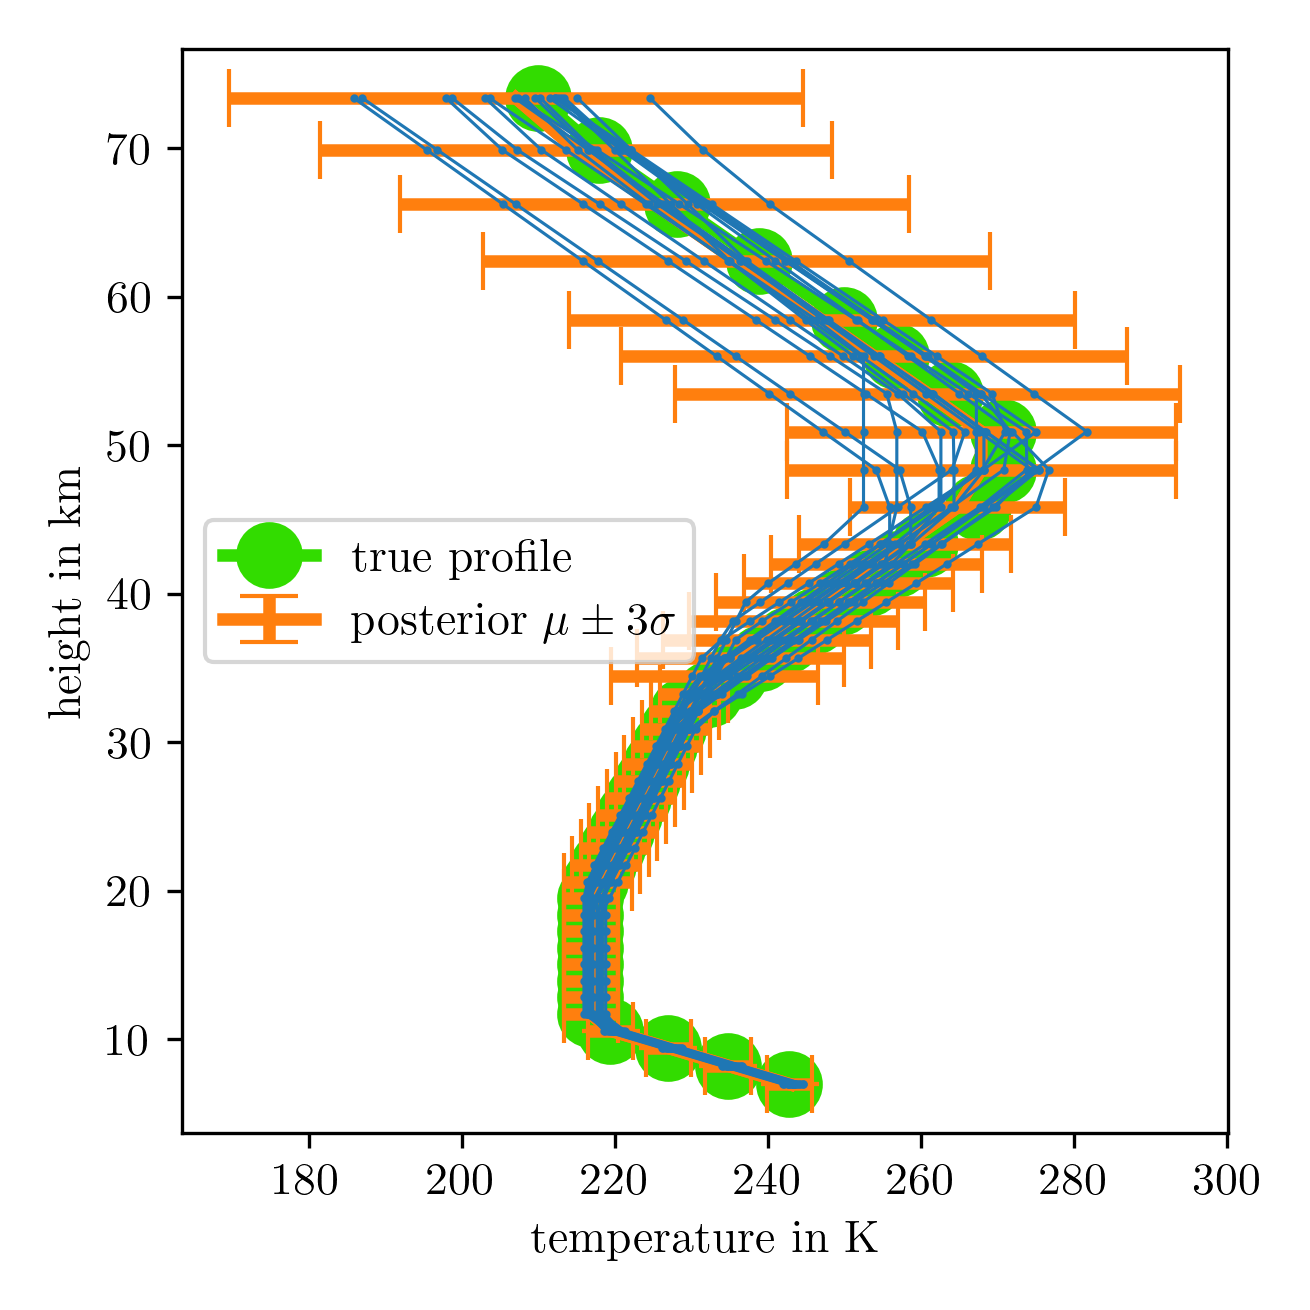
\includegraphics{TempPostMeanSigm.png} 
	\caption[Temperature posterior samples.]{We take samples from the posterior distribution, as plotted in Figures \ref{fig:PostHistTT0} to \ref{fig:PostHistTT3} and plot the corresponding temperature function, see Eq: \ref{eq:tempFunc}. }
	\label{fig:TempPost}
\end{figure}
\cleardoublepage
\begin{figure}[ht!]
	\centering
	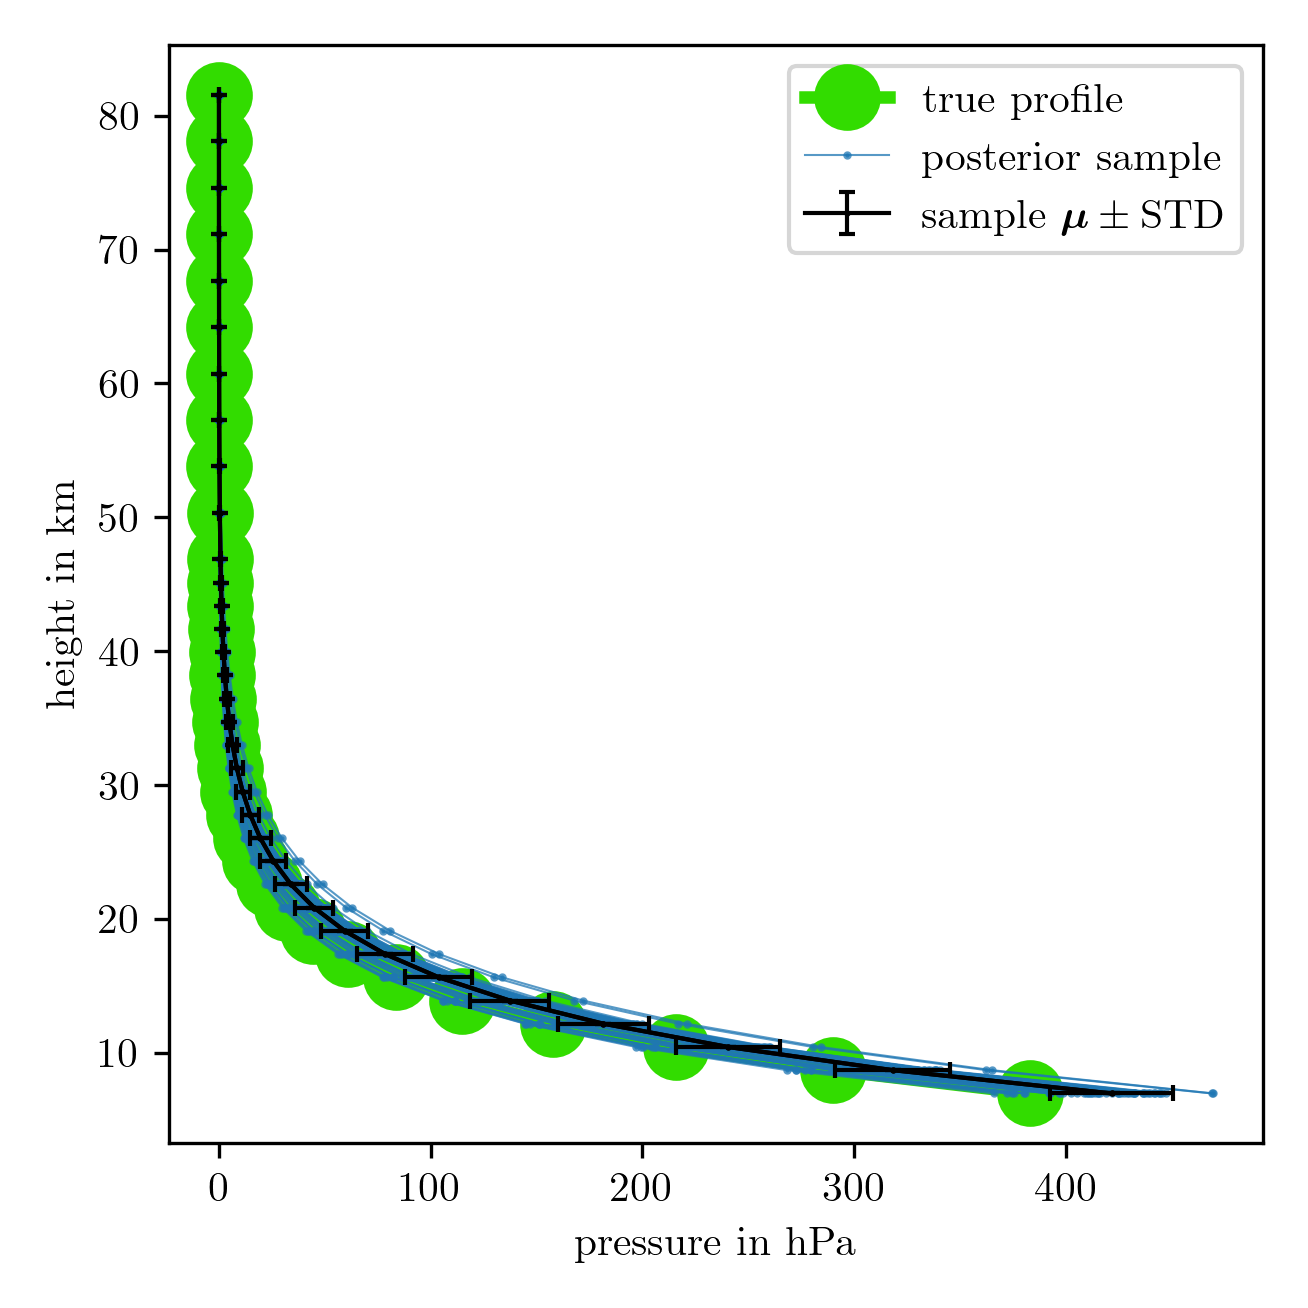
\includegraphics{PressPostMeanSigm.png}
	\caption[Pressure posterior samples.]{We take samples from the posterior distribution, as plotted in Fig. \ref{fig:PostHistTT4} and plot the corresponding pressure function, see Eq: \ref{eq:pressFunc}.}
	\label{fig:PressPost}
\end{figure}

\begin{figure}[h]% will be the left-side figure
		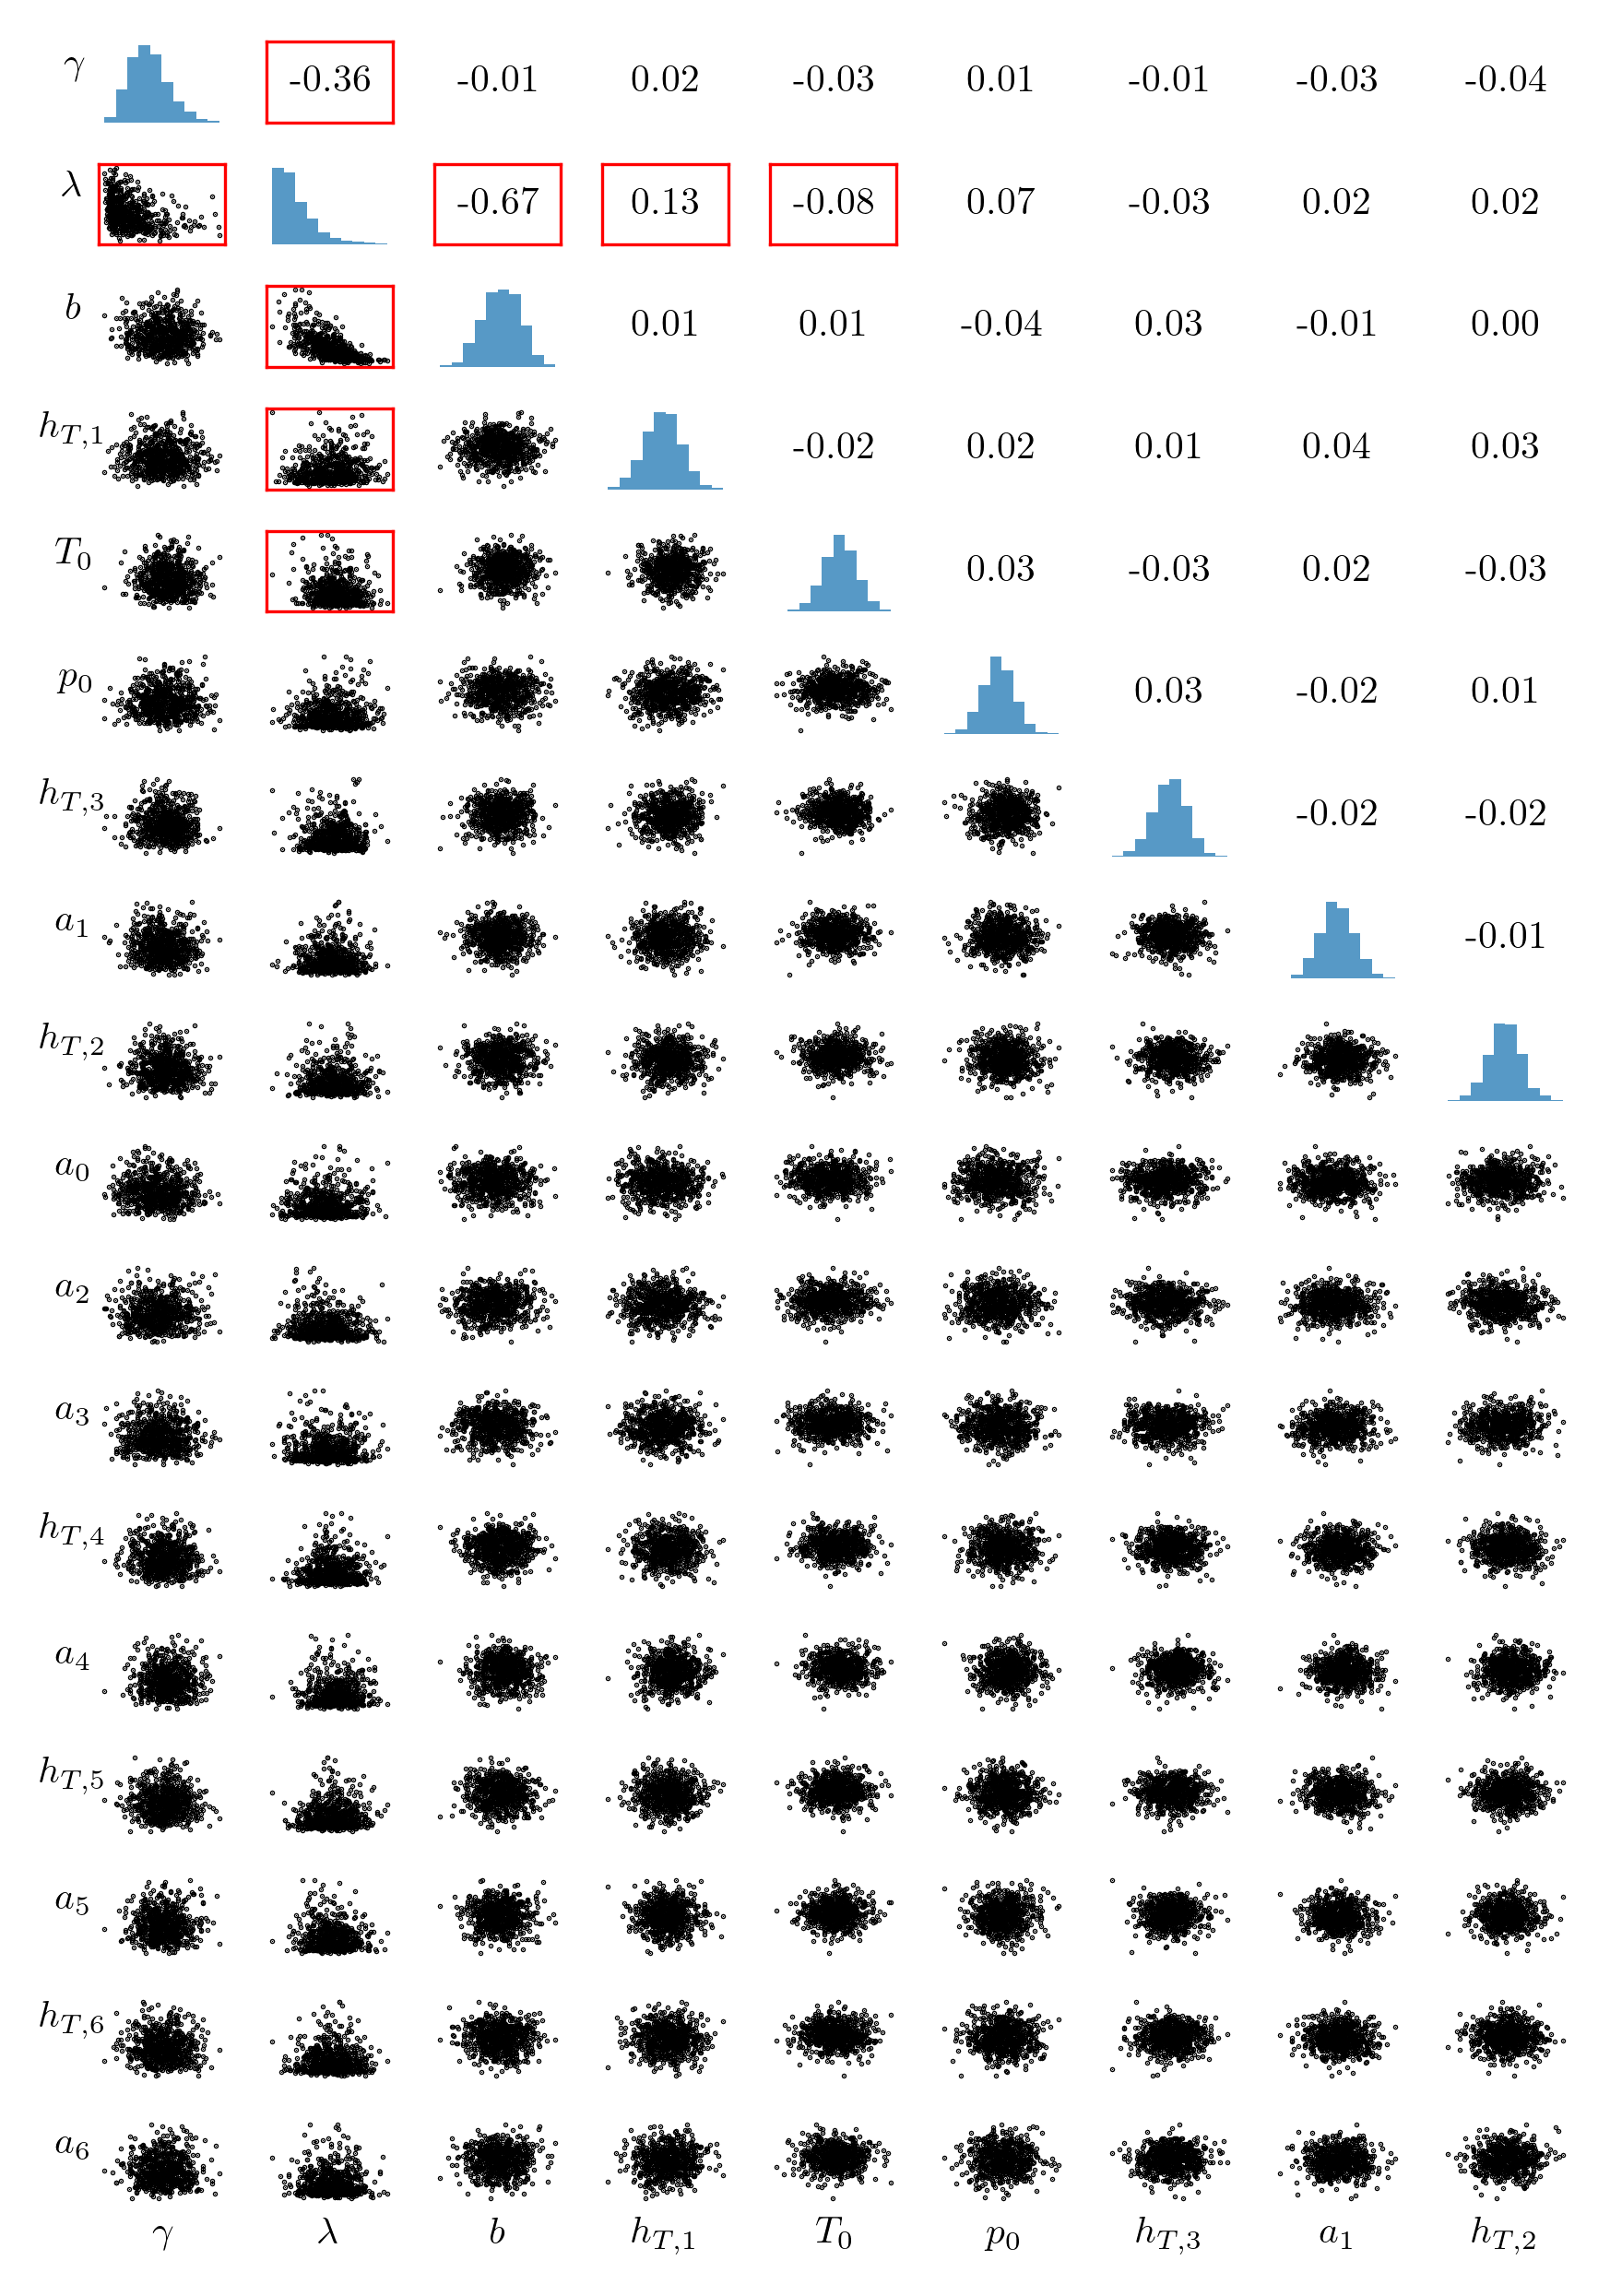
\includegraphics[]{CorrPlot.png}
		\caption[Correlation plot of samples from TT-approximation]{mffjnjf}
\end{figure}
\begin{figure}% will be the right-side figure
		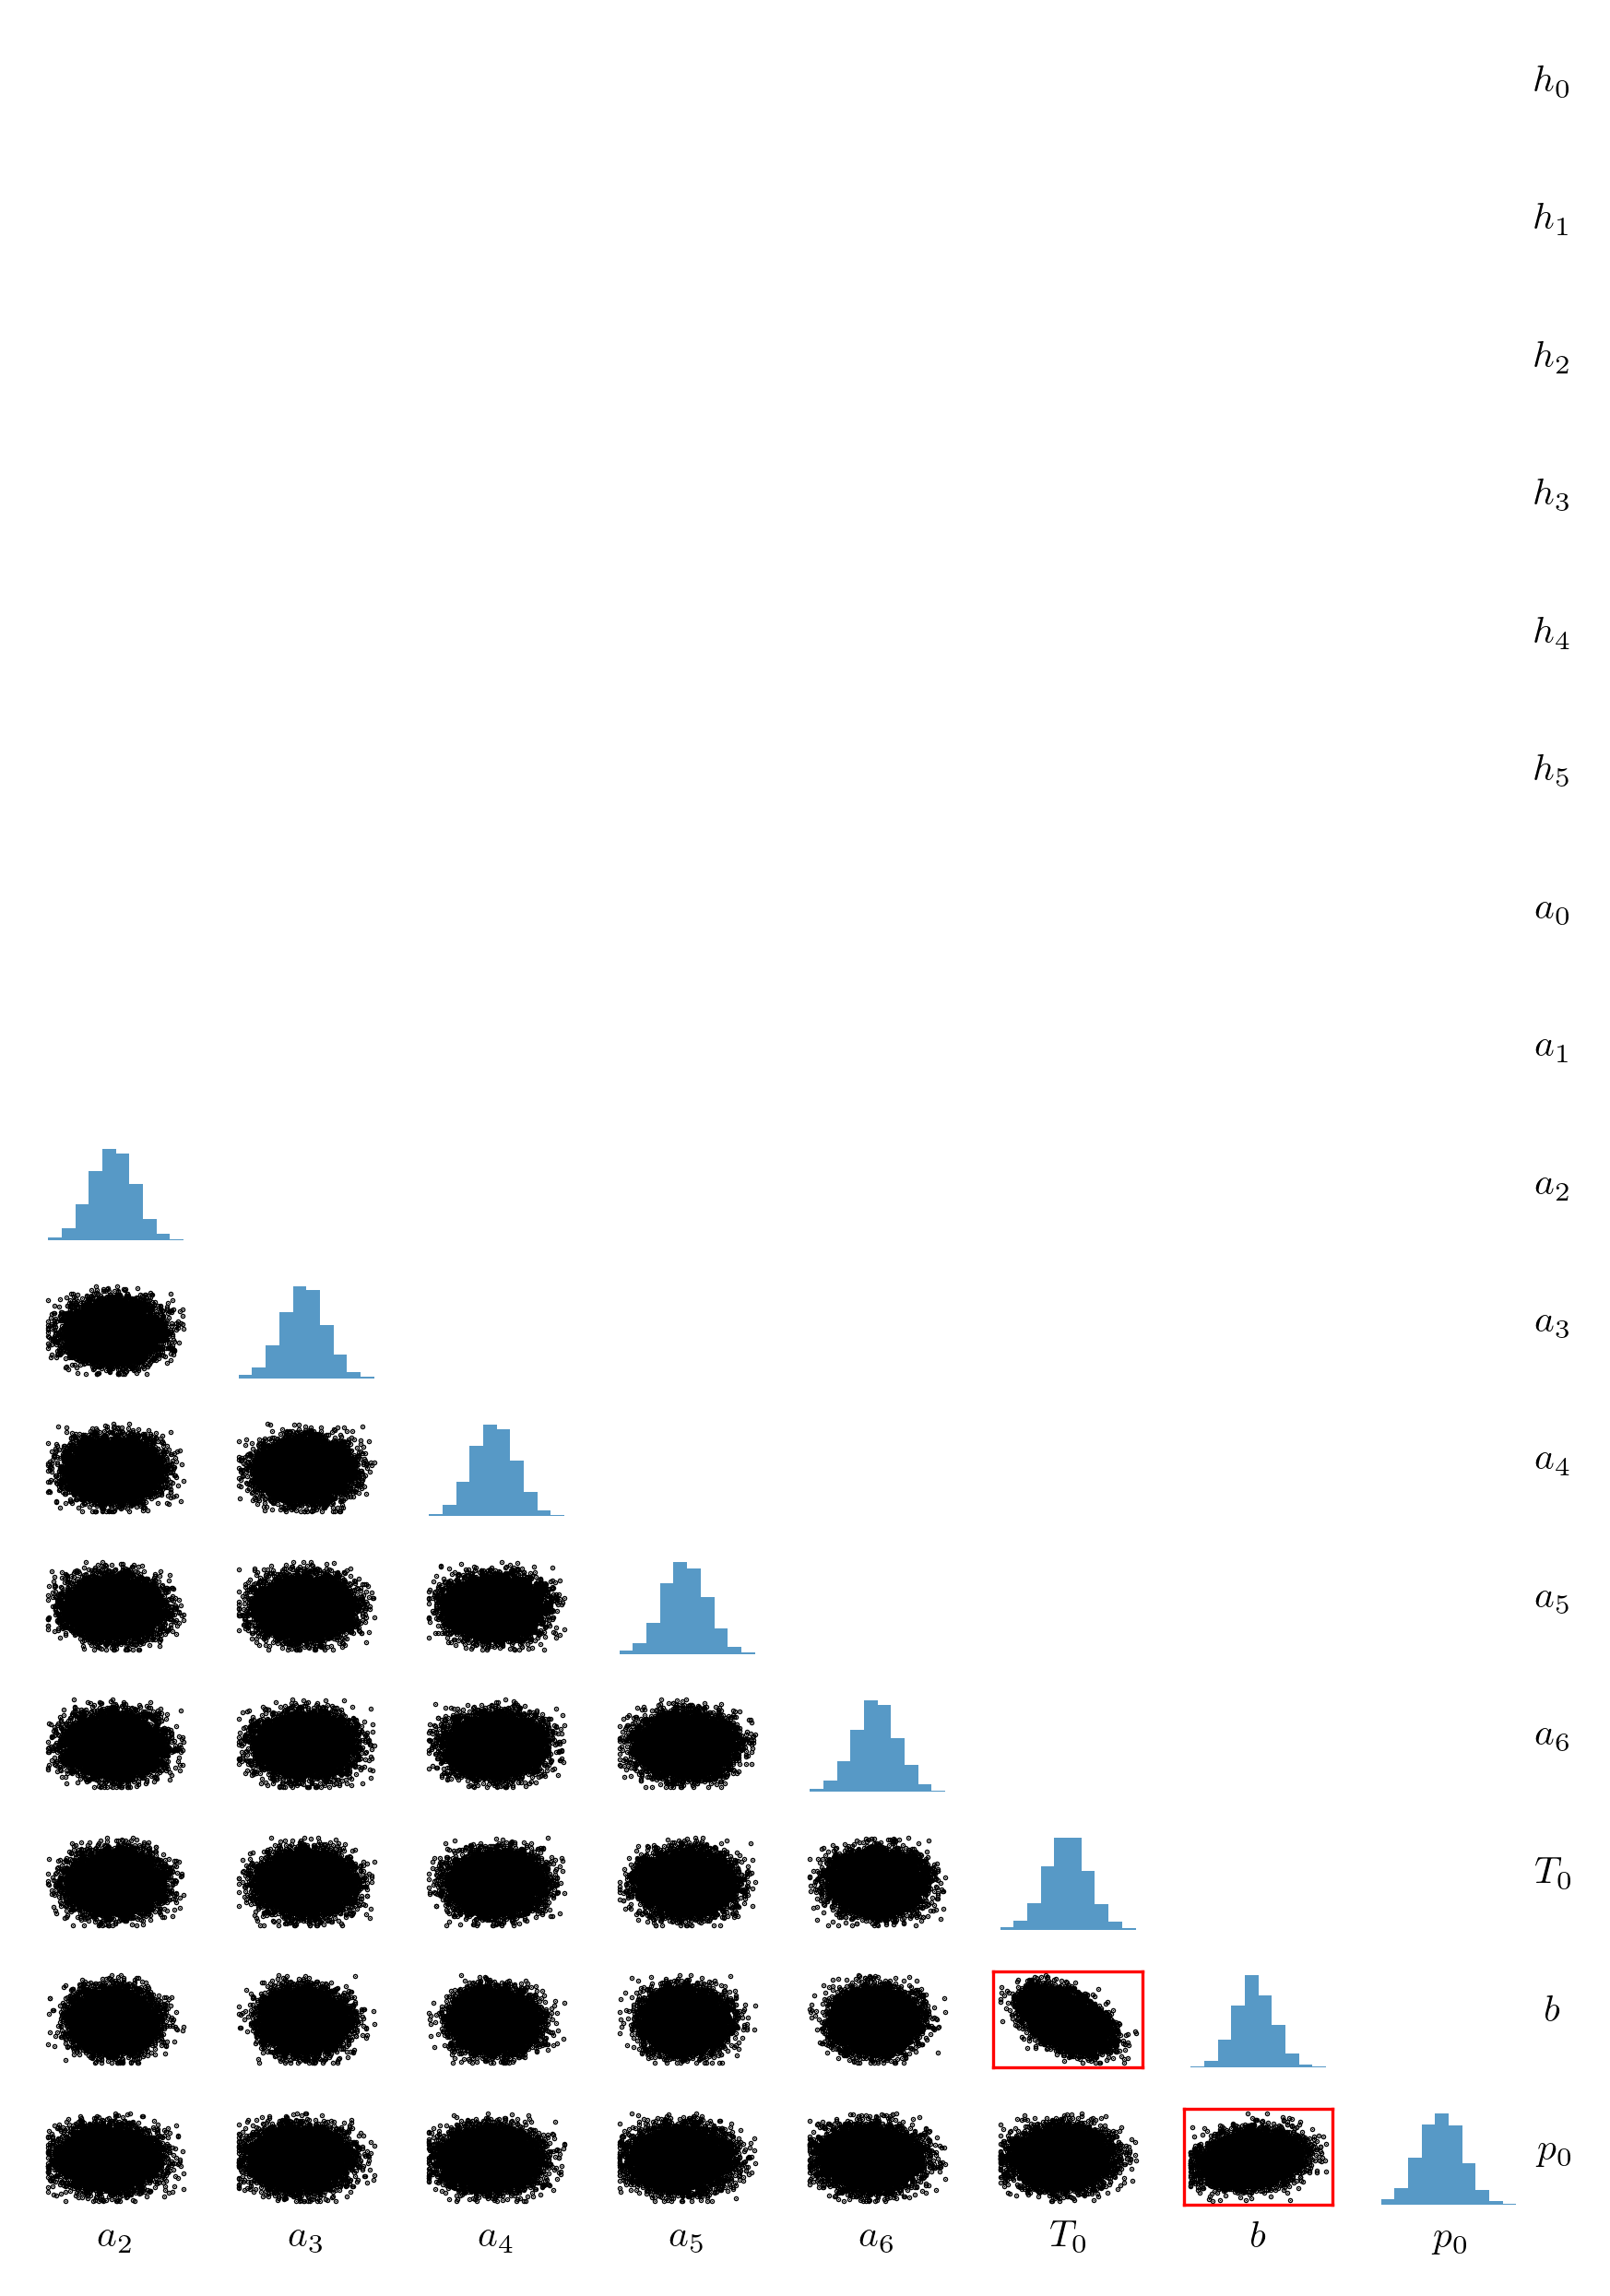
\includegraphics[]{2ndCorrPlot.png}
		\caption*{fhgffg}
\end{figure}
\cleardoublepage
\section{Error analysis}
In this section, we estimate errors due to the function approximations of $f(\lambda)$ and $g(\lambda)$ and how these errors propagate to the marginal posterior.
Additionally, we approximate errors of the TT-approximation as well as Monte-Carlo errors when binning up the samples.

\subsubsection{Error due to approximation of f and g}
\label{sec:fgErros}
When approximating the functions $f(\lambda)$ and $g(\lambda)$, we find that the 3rd-order Taylor series of $f(\lambda)$ and a linear approximation of $g(\lambda)$ in log-space give the smallest error.
The Taylor series truncation error of $f(\lambda)$ is bounded by the fourth order Taylor series $E_f = \underset{\lambda}{\text{arg max}\,} f^{(4)}(\lambda_0)/ 4! \, (\lambda - \lambda_{0} )^4$ and corresponds to an relative error bounded by $20\%$.
Since the maximum absolute error of the approximation $\underset{\lambda}{\text{arg max}\,}|\tilde{g}(\lambda) - g(\lambda) | \approx 1$ corresponds to an relative error of approximately $0.3\%$ and is small compared to $E_f \approx 1e8$ we ignore the approximation error of $g(\lambda)$.
Then the maximum relative propagation error $\underset{\lambda, \gamma}{\text{arg max}\,} 0.5 \gamma  E_f / \log{\pi{(\lambda ,\gamma | \bm{y})}} $ is bound by approximately $5\%$.
\subsubsection{Tensor-train approximation error for the marginal posterior}
We calculate the error of the TT approximation of the marginal posterior with the Wasserstein distance $||x||$.
The wasserstein distance between the normalised true marginal posterior $\pi(\lambda,\gamma|\bm{y})$ and the TT approximation $\tilde{\pi}(\lambda,\gamma|\bm{y})$ is $0.1$.

%When approximating the marginal posterior the maximum relative propagation error $\underset{\lambda , \gamma}{\text{arg max}\,}|\tilde{\pi}(\lambda,\gamma|\bm{y}) - \pi(\lambda,\gamma|\bm{y}) |/ |\pi(\lambda,\gamma|\bm{y})|$ is approximately $100\%$ at $\gamma_{\text{max}}$ and $\lambda_{\text{max}}$, which are the maximum values of the $\lambda$ and $\gamma$ samples and lay in regions with very low probability.
%We consider this error negligible because the absolute error at $\gamma_{\text{max}}$ and $\lambda_{\text{max}}$ is smaller than $10^{-24} \approx 0$.
%Note that one can reduce the maximum errors when approximation $f(\lambda)$ at the mean of $\pi(\lambda,\gamma|\bm{y})$ instead of the modes since $\pi(\lambda | \bm{y})$ is skewed, but we don't see noticeable differences in the conditional posterior $\pi(\bm{x}|\lambda,\gamma,\bm{y})$ when doing so.
%We consider these errors as tolerable.

\subsubsection{Error due to grid size and number of sample bins when calculating the full conditinal mean and covariance}
When we calculate the mean and covariance matrix of the full conditional $\pi(\bm{x}|\bm{y})$ we have to bin up the samples of the marginal posterior $\pi(\gamma, \delta |\bm{y})$ or use a TT approximation on a predefined grid with a certain number of grid points, we like to give an estimate for this error as well.
In doing we bin up samples and use the height $\tilde{\pi}(\bm{\theta}^{(k)}_d)$ for a bin $k = 1, \dots, \text{N}_b$ to calculate the mean $\tilde{\mu}_d = \sum_{\text{N}_b} \tilde{\pi}(\bm{\theta}^{(k)}_d) $.
We compare to the sample mean $\bm{\mu}_d = \sum_{k=1}^N \bm{\theta}^{(k)}_d/N$ and calculate the relative error $||\bm{\mu}_{\text{samp}} -\bm{\mu}_{\text{distr}} ||/ || \bm{\mu}_{\text{samp}} ||$
where $\bm{\mu}_{\text{samp}} =(\tilde{\mu}_1, \dots , \tilde{\mu}_D) $ and equivalently $\bm{\mu}_{\text{distr}} =(\tilde{\mu}_1, \dots , \tilde{\mu}_D) $.
Here $d$ refers to the $D = 16$ hyper-parameters $\gamma, \lambda, h_1, h_2, h_3, h_4, h_5, h_6, a_0, a_1, a_2, a_3, a_4, T_0, p_0, b$.

The relative error behaves proportionally to $1/N$, see Fig. \ref{fig:MCError} and Eq. \ref{eq:MCerr}, and we consider a relative error less than $0.1\%$ good enough.
This happens roughly at a bin size of 25, which is our TT grid size.
Note that we exclude the error due to $\tau_{\text{int}}$ the IACT and that we choose the grid according to the sampled values so that the sampling region is the same as the region in which we approximate the posterior distributions.
.\begin{figure}[ht!]
	\centering
	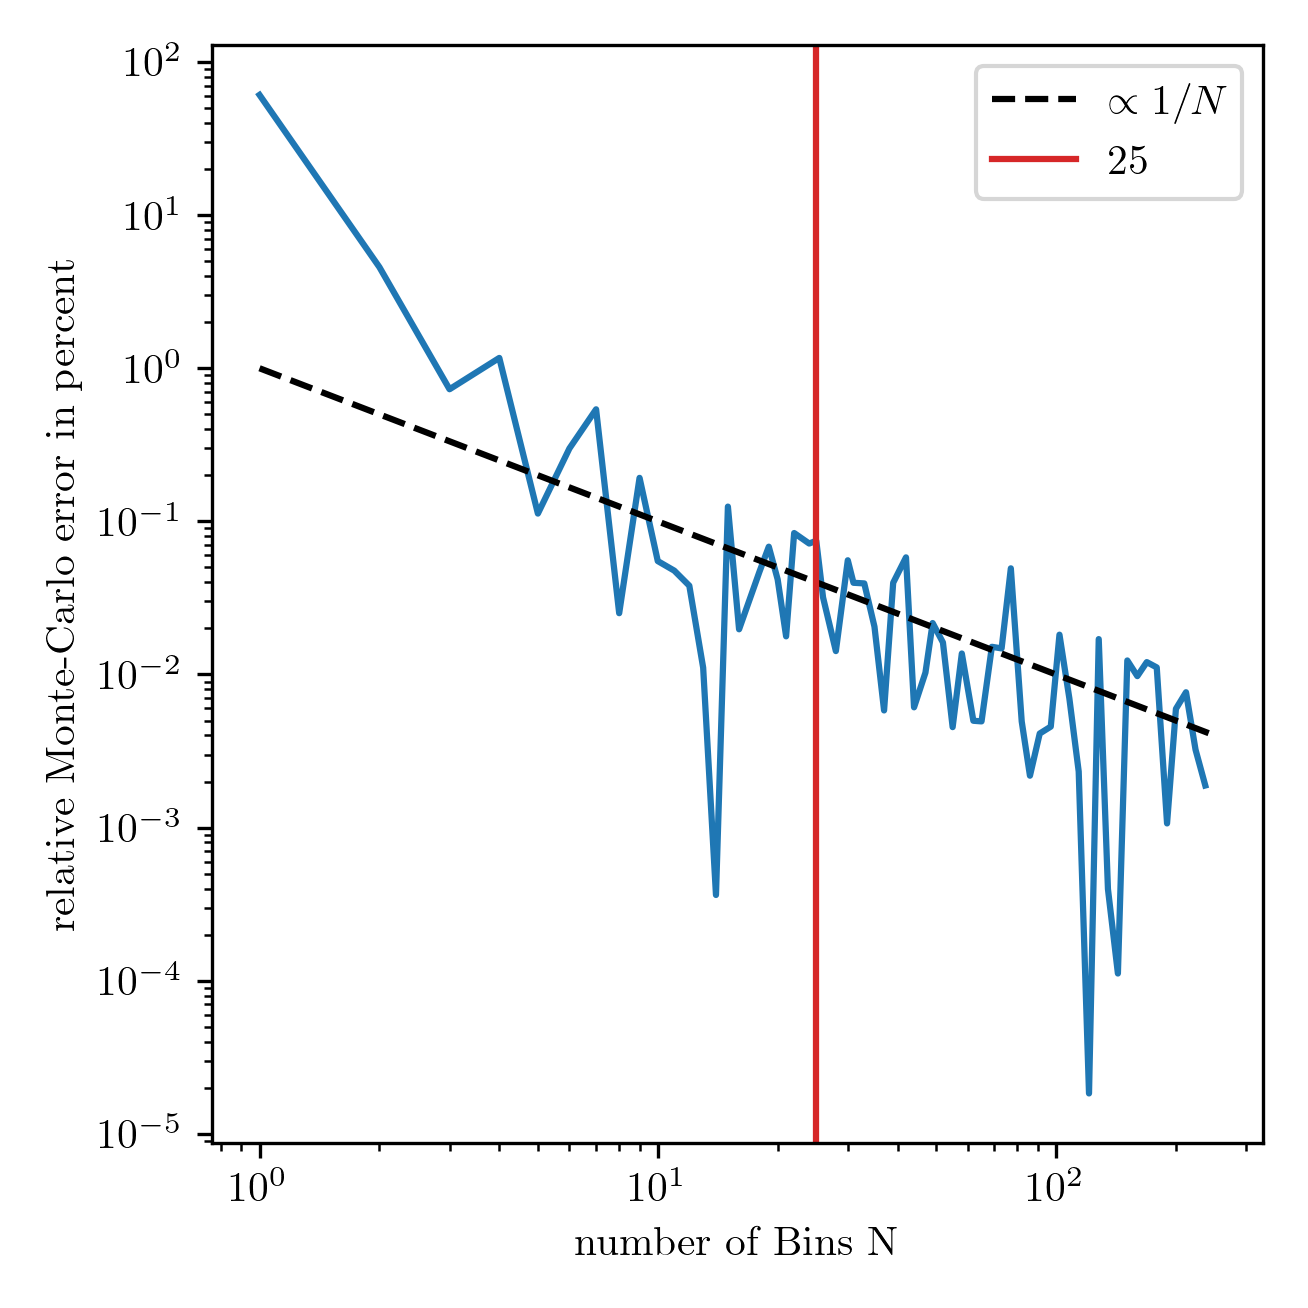
\includegraphics{MeanAssPT.png}
	\caption[Assessment of Monte-Carlo error.]{Assessment of Monte-Carlo error, where we calculate the relative error of the mean due to binning up the samples compared to the sample mean $||\bm{\mu}_{\text{samp}} -\bm{\mu}_{\text{distr}} ||/ || \bm{\mu}_{\text{samp}}||$.}
	\label{fig:MCError}
\end{figure}

